\setcounter{chapter}{0}
\chapter{Elettrostatica}

\section{Propriet\`a elementari dell'interazione elettrica di due cariche}

L'interazione tra corpi ''elettrizati" ha diverse propriet\`a irriducibili. Una di queste \`e lo stato di carica di un corpo che \`e definito da due condizioni:
\begin{itemize}
	\item Carica Positiva (Protoni)
	\item Carica Negativa (Elettroni)
\end{itemize}

che permettono di descrivere una forza d'interazione repulsiva o attrattiva. 
\\
Sperimentalmente si osserva che tutti i corpi (o particelle) possiedono carica e che dati due corpi con lo stesso segno di carica si sperimenta una forza repulsiva e per segni opposti attrattiva. Una delle propriet\`a pi\`u importanti \`e la \textit{conservazione della carica}.
\\
La carica totale di un sistema isolato (ovvero che non scambia carica con l'ambiente), \`e definita dalla somma algebrica delle cariche positive e di quelle negative ed \`e costante.
\begin{equation*}
	Q = \sum q^+ + \sum q^- = \text{cost}
\end{equation*} 
La carica non sono \`e conservata per tutti gli osservatori inerziali, ma \`e anche un invariante relativistico, ovvero la carica totale Q non dipende dall'osservatore.
\\
Un altra propriet\`a importante \`e che la carica \`e \textit{quantizzata}, tale propriet\`a ci dice che in un corpo carico, la carica totale \`e un multiplo intero della carica di un elettrone o di un positrone. Al momento non esiste una spiegazione al motivo per cui la carica sia quantizzata e assuma valori continui.
\\
La materia contiene un numero enorme di protoni ed elettroni $\geq 6 \times 10^{23}/mol$. Una piccola differenza di carica renderebbe la materia non neutra, e dunque elettricamente instabile, dunque la materia in natura possiede carica neutra.

\section{Legge di Coulomb (Elettrostatica)}

L'interazione tra due cariche puntiformi e stazionarie, ovvero fisse l'una rispetto all'altra e nel riferimento del laboratorio, \`e descritta dalla legge di forza 
\begin{equation}
	\bold{F} = k \frac{q_1q_2}{r_{12}^2} \;\hat{\mu}_{r_{12}} \quad \text{dove} \quad \vec{r_{12}} = \vec{r_2} - \vec{r_1}
\end{equation}
che esprime la forza esercitata dalla prima carica sulla seconda.
\\
La dipendeza dal prodotto delle cariche fa si che a seconda del loro segno si abbia il verso dell'interazione.
\begin{itemize}
	\item Per una coppia di cariche (+,-) si ha che $\bold{F}$ \`e attrattiva. 
	\item Per una coppia (+,+) o (-,-) si ha che $\bold{F}$ \`e repulsiva.  
\end{itemize}
Il valore della costante k, e della carica, dipende dalla scelta del sistema di misura. Nel sistema internazionale la carica \`e misurata in Coulomb (C) e la costante k \`e posta nella forma 
\begin{equation*}
	k = \frac{1}{4 \pi \varepsilon_0} = 8,81 \times 10^9 \;  \frac{N m^2}{C} \quad \text{e} \quad \varepsilon_0 = 8.85 \times 10^{-12} \; \frac{C^2}{Nm^2} 
\end{equation*}
il termine $\varepsilon_0$ prende il nome di \textit{costante dielettrica nel vuoto} e il suo valore dipende dalle propriet\`a del mezzo rispetto a cui avviene l'interazione elettrostatica, in questo caso stiamo considerando il vuoto.
\\ 
Utilizziamo l'unit\`a di misura dell'Ampere (A) che rappresenta l'intensit\`a di corrente posta tra due fili paralleli posti a un metro di distanza e che generano una forza di $\mu_0 = 4 \pi \times 10^{-7} \; N$. La carica elementare di un elettrone \`e pari a 
\begin{equation*}
	e = - 1.6 \times 10^{-19} \;C
\end{equation*}
che coincide con quella di un protone, ma con segno opposto.
\\
L'interazione di Coulomb coinvolge oggetti che possiedono massa, ma l'interazione gravitazionale tra le cariche elementari \`e trascurabile.
\subsubsection{Esempio}
Se consideriamo l'interazione tra due protoni distanti 1 metro e ricordando che la costante gravitazionale \`e $G = 6.67 \times 10^{-11} \; \frac{m^3}{Kgs^2}$ e la massa di un protone \`e pari a $m_p = 1.67 \times 10^{-27} \; Kg $ si ha che il rapporto tra forza gravitazionale e di Coulomb \`e 
\begin{equation*}
\frac{F_G}{F_{el}} = \frac{Gm_p^2}{kp^2} \approx 10^{-36}
\end{equation*}

\begin{remark}
Tra le cariche elementari si esercita anche una forza magnetica, associata al momento magnetico elementare della particella ( propriet\`a quantistica associata allo SPIN). Su distanze atomiche, ovvero di un $\mathring{A} = 10^{-10} m$, l'interazione magnetica elementare \`e  $\approx 10^4$ volte meno intensa dell'interazione elettrostatica e a livello macroscopico \`e totalmente trascurabile (l'intensit\`a diminuisce come $\frac{1}{r^3}$).
\end{remark}

\section{Principio di Sovrapposizione}

Consideriamo un sistema costituito da tre cariche $q_1,q_2$ e $q_3$, possiamo calcolare la forza di Coulomb esercitata su coppie distinte 
\begin{equation*}
	\begin{aligned}
		& \bold{F}_{13} = \frac{1}{4\pi \varepsilon_0} \frac{q_1q_3}{r_{13}^2}\hat{\mu}_{13} \\[0.3cm]
		& \bold{F}_{12} = \frac{1}{4\pi \varepsilon_0} \frac{q_1q_2}{r_{12}^2}\hat{\mu}_{12} \\[0.3cm]
		& \bold{F}_{23} = \frac{1}{4\pi \varepsilon_0} \frac{q_2q_3}{r_{23}^2}\hat{\mu}_{23} \\
	\end{aligned}
\end{equation*}
Se vogliamo calcolare la forza su una singola carica, per esempio $q_3$, si ha evidenza sperimentale che la forza complessiva su di essa \`e data da 
\begin{equation*}
	\bold{F}_{3} = \frac{1}{4 \pi \varepsilon_0} \frac{q_1q_3}{r_{13}^2}\hat{\mu}_{13} \; + \; \frac{1}{4\pi \varepsilon_0} \frac{q_2q_3}{r_{23}^2}\hat{\mu}_{23}
\end{equation*}
ovvero \`e somma vettoriale delle forze elettrostatiche dovute a tutte le altre cariche nel sistema.


\subsection{Distribuzioni di carica per corpi continui}

\begin{wrapfigure}{r}{0.5\textwidth}
  \begin{center}
    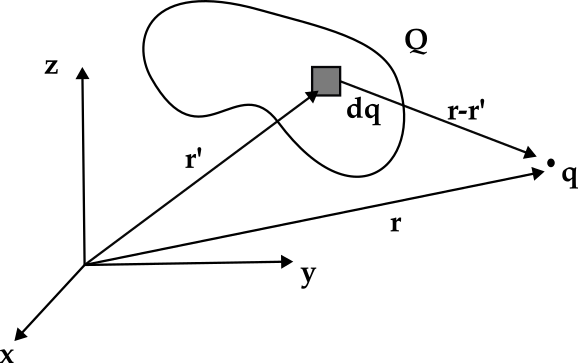
\includegraphics[width=0.4\textwidth]{images/chargeDist}
  \end{center}
\end{wrapfigure}

I sistemi macroscopici sono costituiti da un numero elevato di cariche e tipicamente il suo bilancio \`e neutro, ovvero si ha un egual numero di elettroni e protoni. Quando l'equilibrio viene rotto vengono spostate molte cariche e dunque il problema tipico che viene affrontato \`e quello di determinare la forza esercitata da una distribuzione di carica generica. Per farlo ricorriamo al principio di sovrapposizione. 
\\

\noindent Se consideriamo una carica q interagente con una porzione di carica dq infinitesima di una distribuzione continua Q, abbiamo che la forma esercitata tra le due cariche \`e data da
\begin{equation*}
	d\bold{F} = \frac{1}{4 \pi \varepsilon_0} \frac{qdq}{|\vec{r} -\vec{r'}|^2}\hat{\mu}_{rr'}
\end{equation*}
la forza d'interazione complessiva sar\`a data dall'integrale rispetto alla carica totale della distribuzione della forza infinitesima 
\begin{equation*}
	\bold{F} = \frac{1}{4 \pi \varepsilon_0} \int_{Q} \frac{qdq}{|\vec{r} -\vec{r'}|^2}\hat{\mu}_{rr'}
\end{equation*}
posto $dq' = \rho(\vec{r})dV$ definiamo il termine $\rho(\vec{r})$ come desint\`a volumica di carica e possiamo riscrivere la forza di Coulomb rispetto al volume della distribuzione di carica
\begin{equation*}
	\bold{F} = \frac{1}{4 \pi \varepsilon_0} \int_{V} \frac{\rho(\vec{r})dV}{|\vec{r} -\vec{r'}|^2}\hat{\mu}_{rr'}
\end{equation*}

Se l'elemento di carica considerato dal corpo continuo \`e macroscopicamente piccolo, possiamo considerare le densit\`a di carica funzioni continue rispetto la posizione, mentre se \`e microscopicamente grande le densit\`a sono funzioni regolari della posizione. In sostanza nel primo caso il volume infinitesimo dV considerato possiede un grande quantit\`a di cariche e quindi \`e trascurabili la natura corpuscolare delle cariche e quindi possiamo trattarlo come un elemento continuo.

\subsection{Configurazioni Notevoli di carica}
Le distribuzioni carica non assumono solo forme tridimensionali, ma possono essere superficiali o lineari, per entrambi i casi si definiscono:
\subsubsection{Distribuzione superficiale di carica}

Consideriamo uno strato sottile (di spessore trascurabile) di area S di un materiale. Allora avremo che 

\begin{minipage}{0.6\textwidth}
\begin{equation*}
dq = \rho dV = \rho (tdA) = (\rho t)dA = \sigma dA
\end{equation*}
\end{minipage}
\begin{minipage}{0.4\textwidth}
\centering
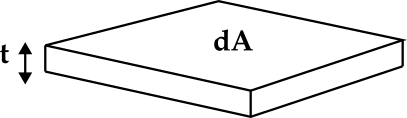
\includegraphics[width=\textwidth]{/areica.png}
\end{minipage}
dove 
\begin{equation*}
	\sigma = \frac{dq}{dA}
\end{equation*}
prende il nome di \textit{densit\`a di carica areica}. La corrispettiva forza esercita da una superficie di carica \`e data dall'integrale di superficie della forza di Coulomb per una carica sonda q 
\begin{equation*}
	\bold{F} = \int_{S}d\bold{F} = \frac{q}{4 \pi \varepsilon_0} \int_{S} \frac{\sigma(\vec{r})dA}{|\vec{r}-\vec{r'}|^2} \mu_{rr'}
\end{equation*}

\subsection{Distribuzione lineare di carica}

Consideriamo un cavo  la cui sezione ha superficie A, e prendiamone un tratto infinitesimo, allora la quanti\`a di carica contenuta sar\`a data da

\begin{minipage}{0.6\textwidth}
\begin{equation*}
dq = \rho dV = \rho (Adl) = (\rho A)dl = \lambda dl
\end{equation*}
\end{minipage}
\begin{minipage}{0.3\textwidth}
\centering
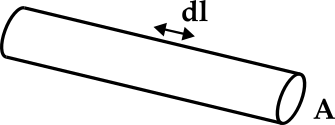
\includegraphics[width=\textwidth]{/lineica.png}
\end{minipage}
\\
dove 
\begin{equation*}
	\lambda = \frac{dq}{dl}
\end{equation*}
prende il nome di \textit{densit\`a lineica di carica}. Se consideriamo una carica sonda q la forza esercitata dalla carica lineare su tale particella sar\`a espressa dalla legge di Coulomb formulata nel seguente modo
\begin{equation*}
	\bold{F} = \int_{L} d\bold{F} = \frac{q}{4 \pi \varepsilon_0} \int_{L} \frac{\lambda(\vec{r'})dl}{|\vec{r} - \vec{r'}|^2} \hat{\mu}_{rr'}
\end{equation*}

\section{Energia di un Sistema di Cariche}

In linea di principio, tutta l'elettorstatica \`e compresa nella legge di Coulomb. Date le cariche e le loro posizioni possiamo ricavare tutte le forze elettriche agenti, o nel caso in cui queste siano in moto per azione di altre forze possiamo determinare la condizione di equilibrio elettrostatica.
\\
Come fattoper la meccanica introduciamo il concetto di energia per l'elettromagnetismo, il che \`e assume un aspetto molto importante dato che le forze elettriche sono di natura \textit{conservativa}.
\\

\noindent Consideriamo un sistema formato da due particelle che inizialmente si trovano ad una grande distanza e dotate di carica $q_1$ e $q_2$. Se ora vogliamo avvicinarle tra loro ad una distanza $\bold{r}_{12}$ quanto lavoro dobbiamo compiere ?
\\
Per rispondere a questa domanda utilizziamo la generica definizione di lavoro, ovvero che il lavoro compiuto in un sistema \`e dato dall'integrale di linea della forza agente sulle cariche.
\begin{equation*}
	W = \int \bold{F} \cdot d\bold{r}
\end{equation*}
dove nel caso di cariche la forza agente \`e per spostare una carica verso l'altra ha la stessa intensit\`a di quella di Coulomb, ma con verso opposto.
\begin{equation}
	W = -\frac{1}{4 \pi \varepsilon_0} \int _{\infty}^{\bold{r}_{12}}\frac{q_1q_2}{\bold{r}^2}d\bold{r} = \frac{1}{4 \pi \varepsilon_0} \frac{q_1q_2}{r_{12}}
\end{equation} 
Di conseguenza abbiamo che il lavoro compiuto sul sistema \`e:
\begin{itemize}
	\item $W > 0$ per cariche dello stesso segno.
	\item $W < 0$ per cariche di segno opposto.
 \end{itemize}
 Dato che la forza \`e conservativa si ha che il lavoro compiuto non dipende dal percorso scelto per avvicinare le due cariche, ma solo dalla posizione iniziale e finale.
 \\
 
 \noindent Supponiamo di introdurre una terza carica $q_3$ all'interno del sistema e di portarla da un punto molto lontano al punto $P_3$ che si trova  a distanza $r_{31}$ per la prima carica e $r_{21}$ per la seconda carica. Il lavoro richiesto per compiere tale operazione \`e 
 \begin{equation*}
 	W_3 = - \int_{\infty}^{P_3}\bold{F}_3 \cdot d\bold{r}
 \end{equation*} 
 Grazie al principio di sovrapposizione abbiamo che la forza totale agente sulla carica $q_3$ \`e data da 
 \begin{equation*}
 	W_3 = - \int (\bold{F}_{31}+\bold{F}_{32}) \cdot d\bold{r} = - \int \bold{F}_{31} \cdot d\bold{r} - \int \bold{F}_{32} \cdot d \bold{r}
 \end{equation*}
 ovvero il lavoro che si compie per portare $q_3$ in $P_3$ \`e la somma del lavoro necessario quando \`e presente solo $q_1$ e di quello necessario quando \`e presente solo $q_2$. Dal risultato ottenuto in (1.2) si ha che
 \begin{equation*}
 	W_3 = \frac{1}{4 \pi \varepsilon_0} \left (\frac{q_1q_3}{r_{31}} + \frac{q_2q_3}{r_{32}} \right )
 \end{equation*}
 Il lavoro totale compiuto per realizzare la distribuzione di tre cariche, che indicheremo con U, \`e 
 \begin{equation}
 	U = W +W_3 = \frac{1}{4 \pi \varepsilon_0} \left (\frac{q_1q_2}{r_{12}} + \frac{q_1q_3}{r_{31}} + \frac{q_2q_3}{r_{32}} \right)
 \end{equation}
 Notare che l'espressione \`e simmetrica rispetto a $q_1,q_2$ e $q_3$ e dunque \`e indipendente da quale carica si considera d'introdurre per ultima. Dunque U non dipende dall'ordine delle cariche con cui si assembla il sistema e non dipende dal percorso che si sceglie per farlo, l'energia totale del sistema dipende unicamente dalla posizione iniziale e finale, come ci si aspetterebbe da un sistema le cui forze agenti sono conservative.
 \\
 Possiamo definire U come \textit{energia potenziale elettrica} del sistema. Quando si definisce un energia potenziale in un sistema vi \`e una certa arbitrariet\`a nella scelta nella sua definizione, in questo caso si \`e scelto come zero di U la configurazione in cui le tre cariche si trovano ad una distanza cos\`i grande tra loro che non vi \`e interazione tra di esse.
 \\
 
 \noindent \`E semplice la generalizzazione del risultato (1.3) ad un sistema costituito da N particelle, \`e sufficiente considerare il lavoro della forza su coppie distinte e sommarlo.
 \begin{equation}
 	U = \frac{1}{2} \sum_{j=1}^N \sum_{k \neq j} \frac{q_jq_k}{r_{jk}}
 \end{equation}
 Il fattore $1/2$ serve ad eliminare i conteggi doppi del lavoro dato che le coppie con ordine (j,k) e (k,j) restituiscono il medesimo risultato e dunque si sommano.

\begin{remark}\
\begin{itemize}
\item 	Se $q_1$ e $q_2$ sono concordi in segno: $U(r) > 0$ le cariche (se non vincolate) si allontanano e l'energia potenziale diminuisce a favore dell'energia cinetica.
\item Se $q_1$ e $q_2$ sono discordi in segno: $U(r) < 0$ le cariche si avvicinano e l'energia potenziale aumenta a sfavore dell'energia cinetica.
\end{itemize}
\end{remark}
\noindent Un sistema le cui cariche a coppie hanno $U(r) < 0$ \`e legato  e occorre compiere del lavoro per separare le cariche. L'energia potenziale per un sistema di questo tipo viene denominata \textit{energia di legame}.

\subsubsection{Esempio - Separazione di una molecola di sale}

Consideriamo la molecola di sale data da $Na^+Cl^-$ costituita da un atomo di sodio (Na) e di cloro (Cl) poste ad una distanza $d \approx 3 \mathring{A}$. Quando l'atomo di sodio e cloro vengono separate a una distanza $r$ molto grande il sistema \`e ben descritto da due cariche puntiformi con carica $|q| = e$. L'energia potenziale (o di legame in questo caso) del sistema \`e data da 
\begin{equation*}
	U (d) = - \frac{e^2}{4 \pi \varepsilon_0 d} \approx - 7.7 \times 10^{-19}J 
\end{equation*}
Se consideriamo un sistema di particelle che pu\`o essere messo in agitazione termica l'energia termica \`e approssimativamente di $\frac{5}{2}kT  = 10^{-20} J$ per una temperatura $T = 300 \;K$. L'energia fornita termicamente \`e di quasi due volte inferiore all'energia necessaria per separare il sodio dal cloro.

\section{Campo Elettrico}

Supponiamo di avere una distribuzione di cariche $q_1,q_2,...,q_n$ fisse rispetto ad un osservatore e di volerne studiare l'interazione con una carica $q_0$. Trascurando la forza d'interazione tra le cariche e considerando solo la forza di Coulomb complessiva sulla nostra carica sonda $q_0$ si ha che 
\begin{equation*}
	\bold{F}_{0} = \sum_{j=1}^N \frac{1}{4 \pi \varepsilon_0}\frac{q_0q_j}{r_{0j}^2}\hat{\mu}_{0j}
\end{equation*}
dove $\bold{r}_{0j}$ \`e la posizione delle cariche rispetto alla posizione di $q_0$. La risultante delle forze risulta essere proporzionale alla carica della particella sonda, se dividiamo per questa quantit\`a la forza totale, otteniamo una grandezza vettoriale che dipende unicamente dalla struttura del sistema iniziale di cariche $q_1,...,q_n$ e dalla posizione della carica $q_0$. Il vettore cos\`i definito prende il nome di \textit{campo elettrico} associato alle cariche $q_1,...q_n$ e viene definito nel seguente modo
\begin{equation}
	\bold{E}(x,y,z) = \frac{\bold{F}_{0}}{q_0} = \frac{1}{4 \pi \varepsilon_0}\sum_{j=1}^N \frac{q_j}{r_{0j}^2}\hat{\mu}_j
\end{equation}
Definito un campo elettrico per qualsiasi carica q, la forza dovuta alla distribuzione di cariche (che abbiamo supposto stazionarie) \`e esprimibile tramite 
\begin{equation*}
	\bold{F}_{q} = q \bold{E}
\end{equation*}
Il campo elettrico associa a ogni punto in un sistema una propriet\`a locale, se conoscia il valore di $\bold{E}$ in una piccola regione, senza bisogno di ulteriori informazioni, conosciamo cosa accadr\`a a qualsiasi carica posta in quella zona, senza necessariamente conoscere come siano distribuite le cariche sorgente.

\subsection{Rappresentazione del Campo Elettrico}

Per visualizzare un campo elettrico \`e necessario associate un vettore, cio\`e, intensit\`a, verso e direzione in ogni punto dello spazio. Inazittuto si consideri il fatto che per per una carica puntiforme la simmetria del campo \`e sferica e la sua direzione \`e data dal segno della carica. Data la simmetria del campo, visto che darne una rappresentazione tridimensionale diventa complicato, possiamo sfruttare tale propriet\`a per darne una raffigurazione bi-dimensionale, che non ne rende inefficacie la descrizione fisica.
\\

\noindent Consideriamo il campo generato da una carica Q positiva (e negativa), e iportizziamo di testarlo con una carica $q_0$, in questo vaso avremo che il campo percepito dalla carica sonda \`e lungo la congiungente e quindi \`e espresso come
\begin{equation*}
	\bold{E}(x,y) = \frac{1}{4 \pi \varepsilon_0} \;
	\frac{Q}{r_0^2} \;\hat{\mu}_{r_0} 
\end{equation*} 
vogliamo riscrivere il campo rispetto alla base di vettori $\{e_1,e_2\}$ che definiscono un sistema ortonormale.

 
\begin{figure}[!ht]
\vspace{0.2in}
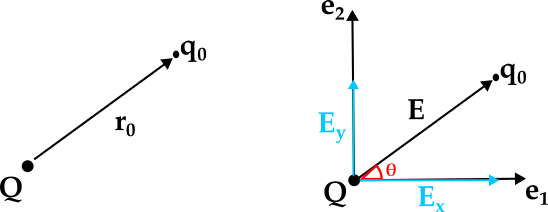
\includegraphics[width= 8cm]{images/decomp}	
\centering
\vspace{0.1in}
\end{figure}
prendendo la posizione di Q come origine del sistema riscriviamo la lunghezza radiale in coordinate cartesiane $r_0^2 = x^2 + y^2$. Le proiezioni del campo rispetto agli elementi della base sono date da 
\begin{equation*}
	\left \{ \begin{array}{l}
		E_x = E \cos\theta \\
		E_y = E \sin\theta 
	\end{array}\right.
\end{equation*}
utilizzando le relazioni fondamentali della tringonometria dove $\cos\theta = \frac{x}{x^2+y^2}$ e $\sin\theta = \frac{y}{x^2+y^2}$ le componenti del campo vettoriale si riscrivono come
\begin{equation*}
	\left \{ \begin{array}{l}
		E_x(x,y) = E  \frac{x}{x^2+y^2} = \frac{Q}{4 \pi \varepsilon_0} \; \frac{x}{(x^2+y^2)^{3/2}}\\
		E_y(x,y) = E \frac{y}{x^2+y^2}  = \frac{Q}{4 \pi \varepsilon_0} \; \frac{y}{(x^2+y^2)^{3/2}}
	\end{array}\right.
\end{equation*}
Conoscendo il valore delle componenti in ogni punto del piano, possiamo definirne direzione, verso e intensit\`a del campo vettoriale. 
\begin{figure}[!ht]
\centering
\begin{minipage}{0.4\textwidth}
  \centering
  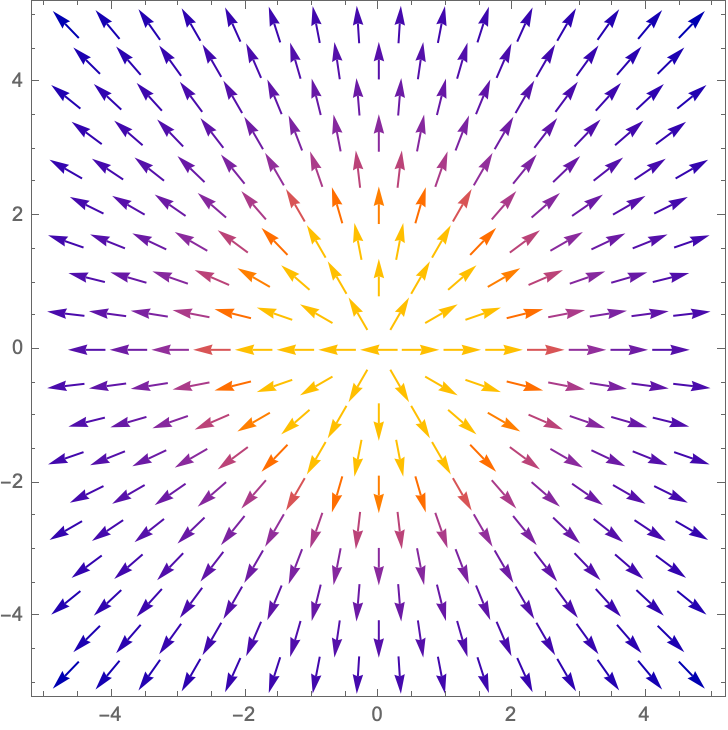
\includegraphics[width=0.8\linewidth]{images/positive}
  \captionof{figure}{Campo Elettrostatico per una sorgente di carica positiva}
\end{minipage}%
\hspace{0.8cm}
\begin{minipage}{0.4\textwidth}
  \centering
  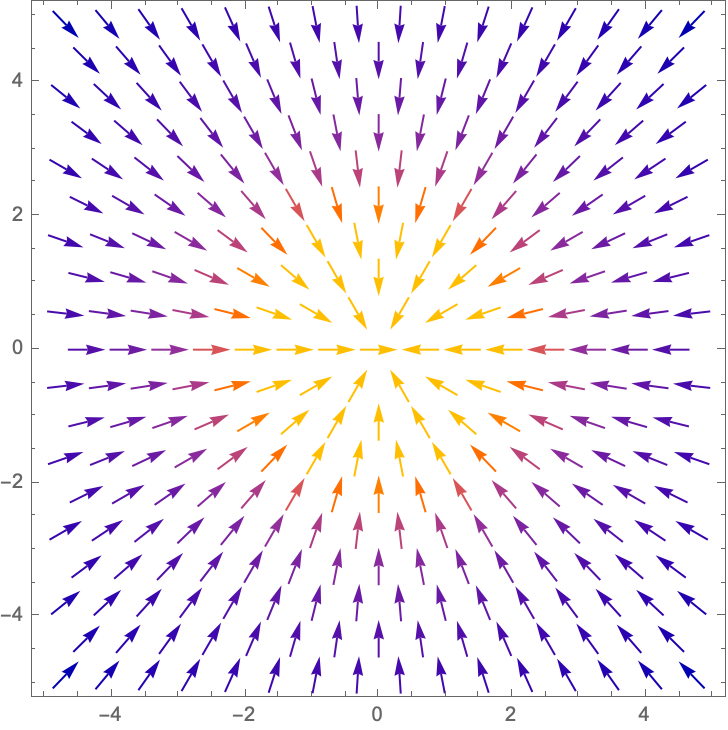
\includegraphics[width=0.8\linewidth]{images/negative}
  \captionof{figure}{Campo Elettrostatico per una sorgente di carica negativa}
\end{minipage}
\end{figure}
 Dalle figura si nota come l'intensit\`a del campo decresca come $\frac{1}{r^2}$ e dunque risultando pi\`u intenso in prossimit\`a della sorgente.
 \\
 \begin{lstlisting}[language = Mathematica]
Mathematica Snippet 

Q = 1.6*10^(-19)
d = 8.854187822*10^(-12)

Ex[q_, x_, y_, x0_, y0_] := 
 q/(4*Pi*d)*((x - x0)/((x - x0)^2 + (y - y0)^2)^(1.5))

Ey[q_, x_, y_, x0_, y0_] := 
 q/(4*Pi*d)*((y - y0)/((x - x0)^2 + (y - y0)^2)^(1.5))

{VectorPlot[{Ex[Q, x, y, 0, 0], Ey[Q, x, y, 0, 0]}, {x, -5, 
   5}, {y, -5, 5}], 
 VectorPlot[{Ex[-Q, x, y, 0, 0], Ey[-Q, x, y, 0, 0]}, {x, -5, 
   5}, {y, -5, 5}]} 
 \end{lstlisting}
 
Dato che il campo elettrico gode del principio di sovrapposizione si ha che per configurazioni di pi\`u cariche si applica lo stesso metodo, sommando le componenti dei campi elettrici generato dalle singole cariche in tutti i punti dello spazio.
\begin{figure}[!ht]
\vspace{0.1in}
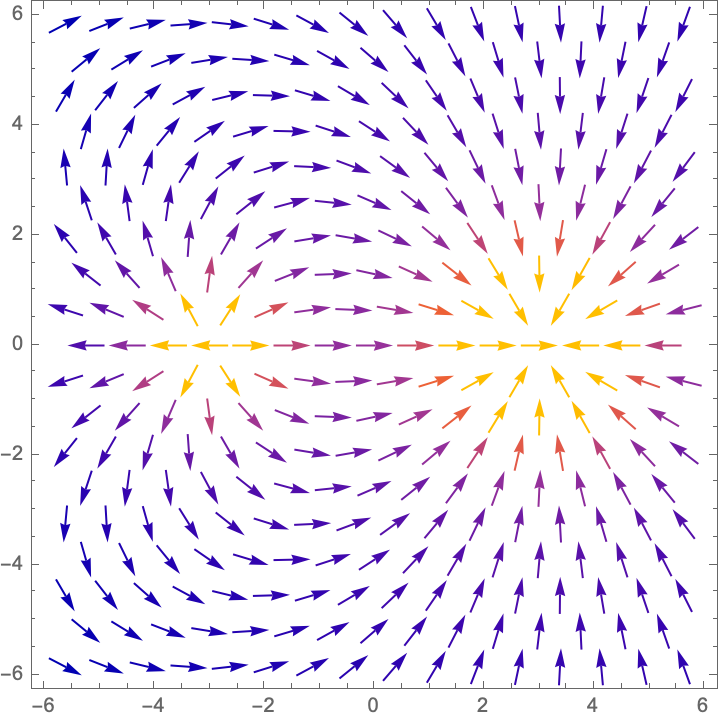
\includegraphics[width = 7cm]{images/interac}	
\centering
\vspace{0.1in}
\caption{Campo generato da una carica Q in (-3,0) e una carica -3Q posta in (3,0)}
\end{figure}

\newpage 
 
\begin{lstlisting}[language = Mathematica]
Mathematica Snippet 

Exx[q1_, q2_, x_, y_, x0_, y0_, x1_, y1_] =  
	Ex[q1, x, y, x0, y0] + Ex[q2, x, y, x1, y1]

Eyy[q1_, q2_, x_, y_, x0_, y0_, x1_, y1_]  = 
	Ey[q1, x, y, x0, y0] + Ey[q2, x, y, x1, y1]

VectorPlot[
{Exx[Q, -3*Q, x, y, -3, 0, 3, 0], Eyy[Q, -3*Q, x, y, -3, 0, 3, 0]}, 
{x, -6, 6}, {y, -6, 6}
]
\end{lstlisting}
Un altro modo per rappresentare un campo, e in questo caso un campo elettrico, \`e utilizzando le linee di flusso (forza). Queste si ottengono risolvendo il sistema di equazioni differenziali 
\begin{equation*}
\left \{\begin{array}{l}
	\frac{dx}{dt}= E_x(x,y)\\
	\frac{dy}{dt} = E_y(x,y)
	\end{array}\right.
\end{equation*}
dove il campo elettrico risulta essere tangente alle soluzioni (x(t),y(t)) di questo sistema. (x,y) descrivono curve regolari e continue, tranne che nei punti di singolarit\`a o nei punti dove il campo \`e nullo. Graficamente l'informazione d'intensit\`a di un campo viene recuperata dal fatto che le linee di forza si addensano in prossimit\`a delle cariche sorgente dove il campo \`e intenso e diventano rarefatte allontanandosi.

 
\begin{figure}[!ht]
\vspace{0.1in}
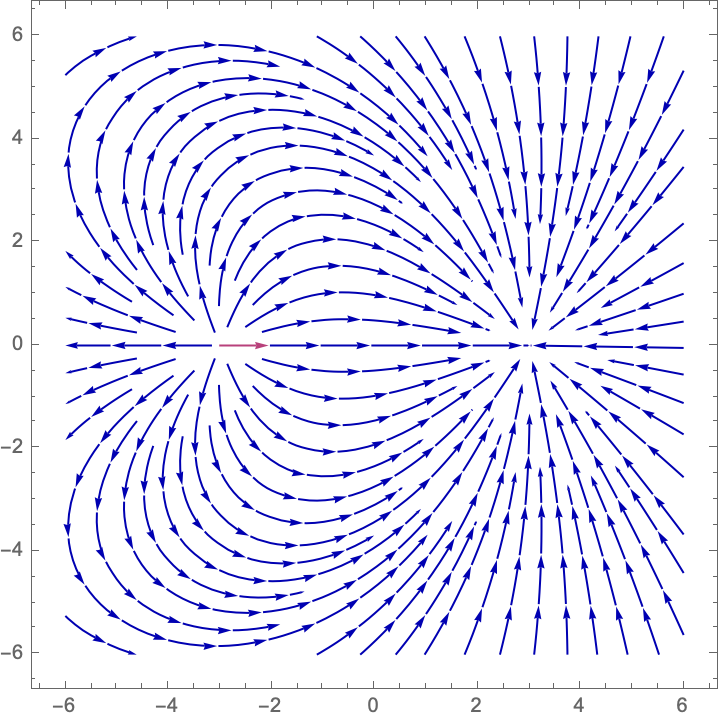
\includegraphics[width = 6cm]{images/stream}	
\centering
\vspace{0.1in}
\caption{Linee di Forza associate per una carica Q in (-3,0) e -3Q in (3,0)}
\end{figure}

\newpage

\begin{lstlisting}[language = mathematica]
Mathematica Snippet 

Exx[q1_, q2_, x_, y_, x0_, y0_, x1_, y1_] = 
	Ex[q1, x, y, x0, y0] + Ex[q2, x, y, x1, y1]
Eyy[q1_, q2_, x_, y_, x0_, y0_, x1_, y1_]  = 
	Ey[q1, x, y, x0, y0] + Ey[q2, x, y, x1, y1]

StreamPlot[
{Exx[Q, -3*Q, x, y, -3, 0, 3, 0], 
  Eyy[Q, -3*Q, x, y, -3, 0, 3, 0]}, 
  {x, -6, 6}, {y, -6, 6}
  ]
\end{lstlisting}

\section{Flusso di un Campo Vettoriale}

La relazione tra campo elettrico e sorgenti pu\`o essere espressa in forma semplice e utile tramite la nozione di \textit{flusso} del campo elettrico attraverso una superficie.

\begin{wrapfigure}{l}{0.4\textwidth}  % "r" means to wrap on the right, width of the figure box
    \centering
    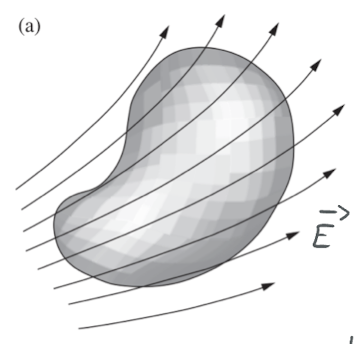
\includegraphics[width=0.25\textwidth]{images/flux}  % Adjust the width as needed
\end{wrapfigure}
\vspace{0.5cm}
\noindent Si immagini di avere una superficie chiusa come in figura in una regione di spazio in cui \`e presente un campo elettrico $\bold{E}(x,y,z)$ generato da una distribuzione di cariche. 

Procediamo con l'affettare tale superficie in piccoli elementi di area $\Delta A_j$ e al centro di ciascuno di essi applichiamo un vettore ortogonale alla superficie la cui intensit\`a \`e data dall'area dell'elemento. Definendo $\bold{\Delta A}_j = \Delta A_j\hat{n}$
dove $\hat{n}$ \`e un versore ortogonale alla superficie considerata e con direzione uscente.

\begin{wrapfigure}{r}{0.4\textwidth}  % "r" means to wrap on the right, width of the figure box
    \centering
    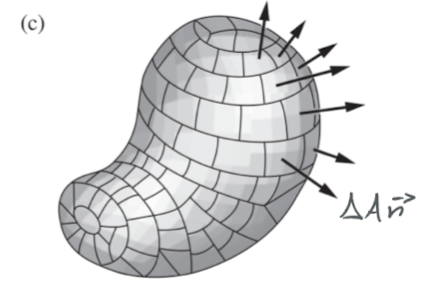
\includegraphics[width=0.3\textwidth]{images/divide}  % Adjust the width as needed
\end{wrapfigure}
Se l'area della porzione di superficie \`e sufficientemente piccola, in quella regione di spazio possiamo considerare il campo elettrico $\bold{E}(x,y,z)$ costante. 
\\

\noindent  Definiamo il flusso del campo elettrico rispetto all'area $\Delta A_j$ come la sua proiezione lungo la direzione del vettore d'area. 
\begin{equation}
	\phi_j = \bold{E} \cdot \bold{\Delta A}_j 
\end{equation} 
Tale definizione prende ispirazione della fluido dinamica dove tale grandezza definisce la rapidit\`a con cui fluisce  il campo elettrico  alla superficie orientata. Infatti se consideriamo un fluido  con velocit\`a $\bold{v}$ in regime stazionario si ha che la portata \`e data da  
\begin{equation*}
	d\phi = \bold{v} \cdot \bold{\Delta A} = \frac{dV}{dt}
\end{equation*} 
Il prodotto scalare recupera ci definisce la proiezione del campo lungo la direzione ortogonale alla superficie, ovvero la superficie efficace attraverso cui fluisce il campo.
 
\begin{figure}[!ht]
\vspace{0.1in}
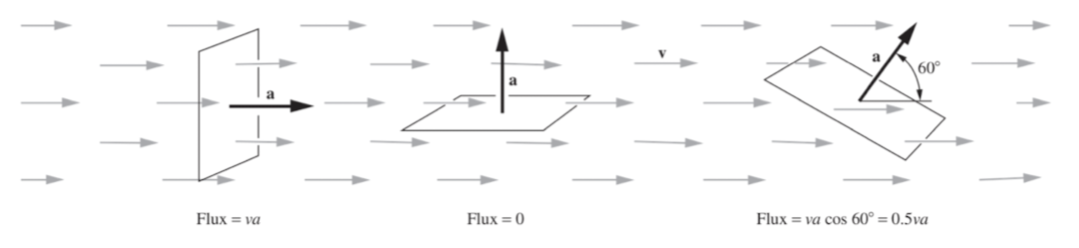
\includegraphics[width = 15.5cm]{images/orient}	
\centering
\vspace{0.1in}
\end{figure}
La definizione di flusso \`e applicabile a qualsiasi funzione vettoriale, indipendentemente dalla variabile fisica che rappresenta.
\\
Il flusso complessivo attravero la superficie \`e ottenuto sommando i singoli contributi
\begin{equation*}
	\begin{aligned}
		& \phi(\bold{E}) = \sum_{j} \bold{E}\cdot \bold{\Delta A}_{j} \quad \text{(Caso Discreto)} & \\[0.5cm]
		& \phi(\bold{E}) = \int_{S}\bold{E} \cdot \bold{dA} \quad \text{(Limite Continuo)}
	\end{aligned}
\end{equation*}

\begin{remark}	
\end{remark}

Notare che, il flusso \`e una funzione che preso un vettore gli associa uno scalare 
\begin{equation*}
	\phi : \mathbb{R}^3 \to \mathbb{R}
\end{equation*}
e inoltre restituisce informazioni sull'insieme del sistema e non locali.

\section{Legge di Gauss}

Consideriamo una regione chiusa dello spazio $ V \subset \mathbb{R}^3$ e consideriamo $S = \partial V$ la superficie di V.  Ipotizziamo che sia presente una distribuzione di carica continua (o discreta) all'interno della regione V, avremo che il flusso del campo elettrico generato attraverso la superficie S \`e dato da 
\begin{equation*}
\begin{aligned}
	& \phi(\bold{E}) = \int_{S} \bold{E} \cdot d\bold{A} = \frac{1}{\varepsilon_0}\int_{V} \rho(\bold{r})dV \quad \text{(Distribuzioni Continue)} & \\[0.5cm]
	& \phi(\bold{E}) = \int_{S} \bold{E} \cdot d \bold{A} = \frac{1}{\varepsilon_0} \sum_{i}q_i
	\quad \text{(Distribuzioni Discrete)}
\end{aligned}
\end{equation*}
Tale relazione prende il nome di \textit{legge di Gauss}. I termini di destra coincidono la quantit\`a di carica complessiva contenuta all'interno della regione V, infatti possiamo definire
\begin{equation*}
	Q = \int_{V} \rho(\bold{r})dV
\end{equation*} 
Con questa legge noto il campo vettoriale ( quindi intensit\`a e geometria) \`e possibile risalire alla carica complessiva delle sorgenti.
\\

\noindent Notare che la forma della \textit{superficie Gaussiana} S non influenza il risultato della Legge di Gauss fin tanto che la carica resta all'interno del volume della regione di spazio V. In sostanza l'integrale del flusso non dipende dalla geometria della superficie, ma dipende dalla sua topologia.
\begin{proof}
	Dimostriamo la non dipendenza della legge di Gauss dalla forma della superficie.
	\\
	I) Consideriamo il campo elettrico dato da una carica puntiforme 
	\begin{equation*}
		\bold{E} = \frac{1}{4 \pi \varepsilon_0} \frac{q}{r^2} \hat{\mu}_{r}
	\end{equation*}
	e che la carica sia racchiusa all'interno di una sfera di raggio R, il flusso attraverso di essa \`e dato da 
	\begin{equation*}
		\phi(\bold{E}) = \int_{S} \bold{E} \cdot d\bold{A} = E(R^2) \int_{S}dA = \frac{1}{4 \pi \varepsilon_0} \frac{q}{R^2} (4\pi R^2) = \frac{q}{\varepsilon_0}
	\end{equation*}
	II) Ora poniamo la regione di spazio sferica in un volume generico V chiuso che la contiene, proiettiamo l'elemento di volume dA della superficie sferica su quella generica V, ottenendo un angolo solido 
	\begin{equation*}
		\Omega = \frac{dA}{R^2} = \frac{da\cos\theta}{r^2}
	\end{equation*}
	 
\begin{figure}[!ht]
\vspace{0.1in}
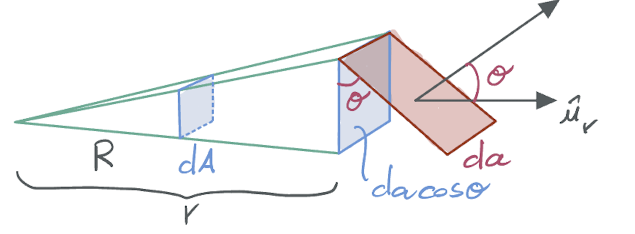
\includegraphics[width = 9cm]{images/solid}	
\centering
\vspace{0.1in}
\end{figure} 
dunque l'area infinitesima della superficie esterna V \`e dara da 
\begin{equation*}
	da = dA\frac{r^2}{R^2 \cos \theta }
\end{equation*}
il campo ha simmetria sferica dunque ha direzione radiale $\hat{\mu}_r$ di conseguenza il flusso attraverso la superficie "da" \`e dato da 
\begin{equation*}
	\phi(\bold{E})_{da} = \bold{E}(\bold{r}) \cdot d\bold{a} = E(r)da \cos \theta = E(R)dA = \phi(\bold{E})_{dA}
\end{equation*}
sommando i contributi infinitesimi si ha che 
\begin{equation*}
	\phi(\bold{E})_{V} = \phi(\bold{E})_{S} = \frac{q}{\varepsilon_0}
\end{equation*}	
\end{proof}
\noindent La legge di Gauss \`e verificata per una qualsiasi distribuzione di carica, se ipotiziamo di avere $q_1,...,q_n$ cariche in una regione chiusa di spazio V si ha che per il principio di sovrapposizione il campo elettrico totale \`e dato da 

\begin{equation*}
	\bold{E} = \sum_{i}\bold{E}_{i}
\end{equation*}
dunque il flusso \`e esprimibile come
\begin{equation*}
	\phi(\bold{E}) = \int_{S} \sum_{i} \bold{E}_i \cdot d\bold{a} = \sum_{i} \phi_i(\bold{E}) = \frac{\sum_{i}q_i}{\varepsilon_0}
\end{equation*}

\begin{prop}
	Se $\bold{F} \not\sim  \frac{1}{r^2}$ la legge di Gauss non \`e valida (La legge di Gauss vale anche per la forza gravitazionale)
\end{prop}
\noindent Si ha che $\phi(\bold{E})_V = 0$ per un campo vettoriale $\bold{E}$ in una regione di spazio chiusa V,  se non ci sono cariche interne oppure se il flusso di cariche esterne alla superficie \`e nullo.
\begin{remark}
Dire che $\phi(\bold{E}) = 0 $ non vuol dire necessariamente che $\bold{E} = 0$.	
\end{remark}
\begin{prop}
\noindent Dato il flusso di un campo vettoriale $\bold{E}$  questo \`e il medesimo per tutte le superfici aperte che sottendono lo stesso angolo solido (e sono dalla stessa parte rispetto alla sorgente del campo elettrico). In sostanza \`e sempre possibile calcolare il flusso attraverso una superficie equivalente che semplifica il calcolo.
\end{prop}

\begin{proof}
	 
\begin{figure}[!ht]
\vspace{0.1in}
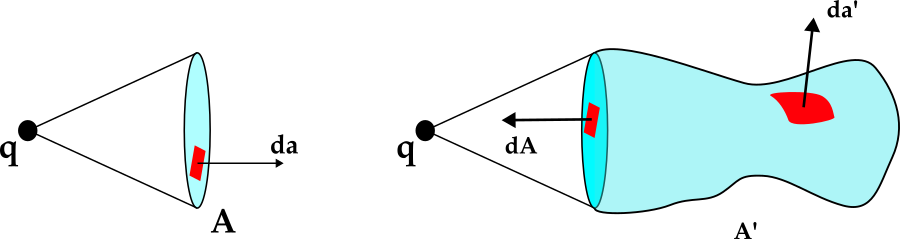
\includegraphics[width = 12cm]{images/same}	
\centering
\vspace{0.1in}
\end{figure}
Consideriamo la superficie chiusa S = A + A', questa non contiene la sorgente di campo "q" e di conseguenza il flusso $\phi_{S}(\bold{E}) = 0$. Se riscriviamo il flusso come
\begin{equation*}
	\phi_S(\bold{E}) = \int_{S = A+A'} \bold{E} \cdot d\bold{A} = \int_{A} \bold{E} \cdot d\bold{A} - \int_{A'} \bold{E} \cdot d\bold{a} = 0
\end{equation*}
dunque si ha che $\phi_{A}(\bold{E}) = \phi_{A'}(\bold{E})$. Il segno negativo compare perch\`e per una superficie chiusa il vettore d'area ha sempre verso uscente rispetto alla superficie)

\end{proof}
\newpage

\subsection{Distribuzione di Carica a Simmetria Sferica}

Consideriamo una distribuzione di carica sferica $\rho$ e di raggio R, all'esterno di essa possiamo approssimare il suo campo a quello di una carica puntiforme, ma come \`e fatto al suo interno? dipende dalla sua distribuzione. Se consideriamo una distribuzione uniforme la carica complessiva \`e data da 
\begin{equation*}
	Q = \frac{4 \pi}{3}R^3 \rho
\end{equation*} 

\begin{wrapfigure}{r}{0.25\textwidth}  % "r" means to wrap on the right, width of the figure box
    \centering
    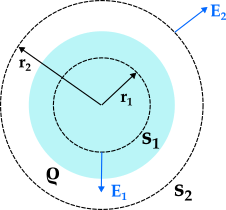
\includegraphics[width=0.3\textwidth]{images/spheric}  % Adjust the width as needed
\end{wrapfigure}

\noindent Consideriamo la superficie sferica S1 come in figura, con centro nell'origine, e raggio $r_1 < R$, la carica contenuta all'interno sar\`a data da 
\begin{equation*}
	Q_{int} = \int_{V}dV\; \rho = \int_{0}^{r_1}dr \; r^2 \int_{0}^{2\pi}d \theta \int_{0}^{\pi}d\varphi \; \sin \varphi = \frac{4 \pi}{3}\rho \; r_1^3 
\end{equation*}
Applicando la legge di Gauss abbiamo che 
\begin{equation*}
\phi(\bold{E}) = \int_{S_1} \bold{E} \cdot d\bold{a}  =	\frac{4 \pi}{3}\rho \; r_1^3 
\end{equation*}
e dunque il campo elettrico sulla superficie $S_1$ \`e data da
\begin{equation*}
	\bold{E}(r_1) = \frac{\rho \; r_1}{3 \varepsilon_0} \hat{\mu}_{r} \quad r_1 \leq R
\end{equation*}

\begin{wrapfigure}{l}{0.4\textwidth}  % "r" means to wrap on the right, width of the figure box
    \centering
    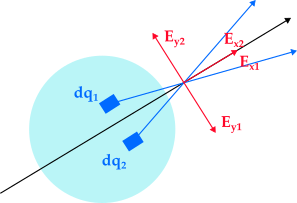
\includegraphics[width=0.4\textwidth]{images/sym}  % Adjust the width as needed
\end{wrapfigure}

L'informazione sulla direzione radiale del campo $\hat{\mu}_{r}$ \`e facilmente recuperabile osservando la simmetria del problema. Consideriamo un sistema di riferimento che divida in due parti simmetriche la sfera, se consideriamo due porzioni di carica $dq_1$ e $dq_2$ su di essa  e li facciamo interagire con una carica sonda $q_0$,posta in un punto che rende equidistanti le cariche, avremo che il campo $\bold{E}$ ha direzione lungo la congiungente $\hat{\mu}_{r0}$ decomponendo rispetto al sistema di riferimento le componenti angolari si eliminato, avendo segni opposti e pari intesit\`a
\begin{equation*}
	E_{y2} + E_{y1} =0
\end{equation*}
e restano solo quelle della componente radiale che si sommano
\begin{equation*}
	\sum_{i}E_{xi} = R_{x}
\end{equation*}
dunque possiamo concludere che il campo abbia direzione radiale.

\begin{wrapfigure}{r}{0.4\textwidth}  % "r" means to wrap on the right, width of the figure box
    \centering
    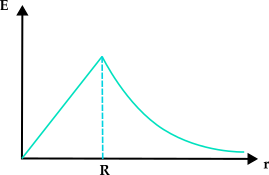
\includegraphics[width=0.4\textwidth]{images/gsphera}  % Adjust the width as needed
\end{wrapfigure}
\vspace{0.5cm}
\noindent Possiamo riassumere i risultati ottenuti per la variazione d'intensit\`a del campo in funzione della posizione radiale, nel seguente modo

\begin{equation}
	\bold{E}(r) = \left \{ \begin{array}{l}
	\frac{Q}{4 \pi \varepsilon_0}\frac{1}{r^2} \hat{\mu}_{r} \quad r >R \\[0.5cm]
	\frac{\rho \; r}{3 \varepsilon_0} \hat{\mu}_{r} \quad r \leq R
	\end{array}\right.
\end{equation}
\newline

\noindent Osserviamo che il campo elettrico \`e continuo in $r=R$, ma la derivata prima $\frac{dE}{dr}$ no, come si osserva dal grafico.

\subsection{Distribuzione di carica a Simmetria Cilindrica (Filo "infinito")}

\begin{wrapfigure}{r}{0.4\textwidth}  % "r" means to wrap on the right, width of the figure box
    \centering
    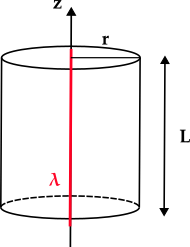
\includegraphics[width=0.25\textwidth]{images/wire}  % Adjust the width as needed
\end{wrapfigure}

Consideriamo una distribuzione di carica lineica $\lambda$ con estensione infinita lungo la direzione z. Attorno ad essa definiamo una superficie Gaussiana cilindrica di raggio $r$ e lunghezza L. La quantit\`a di carica racchiusa sar\`a dara da 
\begin{equation*}
	Q = \frac{\lambda L }{\varepsilon_0}
\end{equation*}
Per ragioni di simmetria il campo elettrico ha simmetria radiale $\hat{\mu}_{r}$. Questo vuol dire che le due basi del cilindro non contribuiscono all'integrale di flusso dato che $\bold{\hat{z}} \cdot \bold{\hat{r}} = 0$. Dunque applicando la legge di Gauss si ha che 
\begin{equation*}
	\int_{S}\bold{E} \cdot d\bold{A} = E(r)2\pi L = \frac{\lambda L}{\varepsilon_0}
\end{equation*}
e quindi il campo elettrico \`e dato da 
\begin{equation}
	\bold{E}(r) = \frac{\lambda}{2\pi \varepsilon_0}\frac{1}{r} \; \hat{\mu}_{r}
\end{equation}
Si osserva che per una distribuzione di carica lineare $\bold{E} \sim \frac{1}{r}$ a differenza di quella di una carica puntiforme il cui campo decresce come $\frac{1}{r^2}$. Quindi l'intensit\`a del campo diminuisce molto pi\`u lentamente.
\\

\noindent Il campo ottenuto \`e una buona approssimazione per $r << L$, dove L \`e la lunghezza del filo. In generale, per un filo finito si ha che la componente angolare del campo $E_{\varphi} = 0$ come nel caso infinito, ma la componente $E_{z} \neq 0$. Il sistema \`e simmetrico per riflessione solo rispetto al punto medio del filo. A distanza infinita il campo risulta essere sferico (possiamo approssimare il filo ad una carica puntiforme) mentre in sua prossimit\`a ha simmetria clindrica e direzione radiale.

\subsection{Distribuzione di Carica di Superficie e Discontinuit\`a}

\begin{wrapfigure}{r}{0.5\textwidth}  % "r" means to wrap on the right, width of the figure box
    \centering
    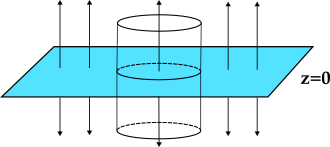
\includegraphics[width=0.5\textwidth]{images/plane}  % Adjust the width as needed
\end{wrapfigure}

Consideriamo un piano infinito, con posizione z = 0, su cui \`e presente una distribuzione di carica superficiale $\sigma$. Prendiamo una superficie Gaussiana cilindrica, con asse perpendicolare al piano come in figura. La direzione del campo elettrico \`e lungo la perpendicolare al piano $\hat{\bold{z}}$. 
\begin{equation*}
	\bold{E}(z) = E(z) \bold{\hat{z}}
\end{equation*}
Inoltre il campo elettrico per $z>0$ deve avere direzione opposta a quella del campo per $z < 0$, e dunque $E(z) = - E(-z)$.
\\

\noindent L'integrale di superficie \`e nullo lungo la superficie laterale del cilindro e gli unici contributi sono dati dalle sue basi, che ipotizziamo avere area A. Utilizzando la legge di Gauss si ha che 
\begin{equation*}
	\int_{S} \bold{E} \cdot d \bold{A} = E(z)A -E(-z)A =2E(z)A = \frac{\sigma A}{\varepsilon_0}
\end{equation*}
In modulo il campo elettrico di una distribuzione di carica per un piano infito \`e dato da 
\begin{equation}
	E(z) = \frac{\sigma}{2\varepsilon_0}
\end{equation}
Il campo elettrico \`e indipendente dalla distanza della carica sonda dal piano. Questo \`e dovuto dal fatto che il piano \`e infinito. e dunque pi\`u ci si allontana, pi\`u superficie diventa visibile.

\begin{figure}[!ht]
\centering
\begin{minipage}{0.5\textwidth}
  \centering
  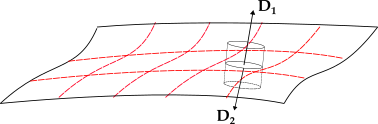
\includegraphics[width= 0.9\linewidth]{images/surface}
  \captionof{figure}{La componente normale del campo elettrico \`e discontinua.}
\end{minipage}%
\hspace{0.8cm}
\begin{minipage}{0.4\textwidth}
  \centering
  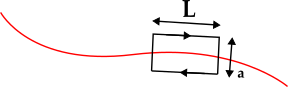
\includegraphics[width=0.8\linewidth]{images/path}
  \captionof{figure}{La componente tangenziale del campo elettrico \`e continua}
\end{minipage}
\end{figure}

Un altro importante fatto \`e che il campo elettrico non \`e continuo rispetto alle due facce del piano per una distribuzione di carica costante. Si ha che 
\begin{equation*}
	E(z \to 0^+) - E(z \to 0^-) = \frac{\sigma }{\varepsilon_0}
\end{equation*}
Tale risultato non dipende dal fatto che il piano sia finito, infatti pu\`o essere tranquillamente esteso a qualsiasi superficie con distribuzione di carica $\sigma$. Inoltre non \`e necessario che $\sigma $ sia costante  e che il campo $\bold{E}$ sia parallelo alla normale $\bold{\hat{n}}$ per ogni punto della superficie. Infatti per una superficie generica, in qualsiasi suo punto possiamo definire un cilindro Gaussiano e ripetere i calcoli per una superficie planare. Se denotiamo con $\bold{E}_{\pm}$ il campo elettrico per entrambe le parti della superficie si ha che 
\begin{equation}
	\bold{\hat{n}} \cdot \bold{E}_{+} - \bold{\hat{n}} \cdot \bold{E}_{-} = \frac{\sigma}{\varepsilon_0}
\end{equation}
e dunque il campo elettrico risulta essere discontinuo rispetto alla perpendicolare per qualsiasi superficie. In contrasto si ha che il campo tangente alla superficie \`e continuo. Per verificarlo basta considerare la circuitazione C con lato L parallela alla superficie e altezza "a" rispetto la perpendicolare.
\begin{equation*}
	\int_{C} \bold{E} \cdot d \bold{r} = LE(z')-LE(z'') = 0 
\end{equation*}
dato che $\bold{E} \cdot \bold{a} = 0$ e questo dimostra la continuit\`a delle componente parallela.

\subsection{Coppia di Piani}

\begin{wrapfigure}{r}{0.5\textwidth}  % "r" means to wrap on the right, width of the figure box
    \centering
    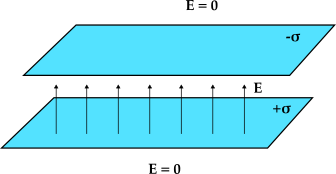
\includegraphics[width=0.5\textwidth]{images/double_plane}  % Adjust the width as needed
\end{wrapfigure}

Si consideri una coppia di piani infiniti rispettivamente a $z = 0$ e $z=a$, che possiedo una distribuzione di carica superficiale $\pm \sigma$ come in figura. Per calcolare il campo elettrico \`e sufficiente applicare il principio di sovrapposizione, considerando il campo generato dai singoli piani. Dato che un campo \`e dato dall'espressione (1.9), tenendo conto di segni e direzione si ha che 
\begin{equation}
	\bold{E} = \frac{\sigma}{\varepsilon_0} \quad 0<z<a
\end{equation}
e $\bold{E} =0$ per $z \in (-\infty,a) \cup (a,+\infty)$.

\section{Potenziale Elettrostatico. Gradiente}

\subsection{Tensione. Differenza di Potenziale Elettrostatico}
Quando su una carica $q_0$ agisce una forza $\bold{F}$ di qualsiasi natura, non necessariamente elettrostatica, ma per esempio dovuta a processi chimici o meccanici, possiamo sempre definire un campo elettrico $\bold{E}$, che prende il nome di \textit{campo elettromotore} ed \`e definito come
\begin{equation*}
	\bold{E} =  \frac{\bold{F}}{q_0} \Rightarrow \bold{F} = q_0 \bold{F}
\end{equation*}
 Notare che l'espressione ottenuta \`e uguale a quella discussa per la forza di Coulomb, ma in questo caso la si sta generalizzando a tutti i tipi di forze che possono agire su una carica. Il lavoro compiuto dalla forza $\bold{F}$ lungo un cammino $d \bold{s}$ \`e dato dal suo integrale linea 
 \begin{equation*}
 	W = \int_{C} \bold{F} \cdot d\bold{s} = q_0 \int_{C} \bold{E} \cdot d\bold{s}
 \end{equation*}
definiamo tensione elettrica tra due punti A e B lungo un percorso C il lavoro per unit\`a di carica  
\begin{equation*}
	\mathcal{E} = \frac{W}{q_0} = \int_{C}\bold{E} \cdot d\bold{s}
\end{equation*}
 In generale per un circuito chiuso C il lavoro \`e non nullo
\begin{equation*}
	W = \oint_{C} \bold{F} \cdot d\bold{s} = q_0 \oint_{C} \bold{E} \cdot d\bold{s} = q_0 \mathcal{E}
\end{equation*} 
L'integrale 
\begin{equation*}
	\mathcal{E} = \oint_{C} \bold{E} \cdot d \bold{s}
\end{equation*}
prende il nome di \textit{forza elettromotrice}. Dipende dal percorso e dalla natura del campo $\bold{E}$, ma non dalla carica $q_0$. Se il lavoro lungo un percorso chiuso C risulta essere nullo si ha la forza \`e di natura conservativa. Non dipende effettivamente dal percorso, ma solo dalla posizione di partenza e di arrivo.
\\

\noindent Nel caso di un campo $\bold{E}$ originato da una distribuzione di carica nello spazio, si ha che la forza esercitata su una carica sonda $q_0$ \`e quella di Coulomb ed \`e di natura conservativa, ovvero il suo integrale di linea su un circuito chiuso \`e nullo. Se forze di questo tipo il loro lavoro \`e dato dal teorema fondamentale del calcolo integrale in cui si considera la differenza delle primitive valutate ai due capi del percorso.
\begin{equation*}
	\int_{A}^{B} \bold{E} \cdot d \bold{s} = F(B) -F(A)
\end{equation*} 
Nel caso della forza di Coulomb tale grandezza prende il nome di \textit{differenza di potenziale elettrostatico}. Dato che la carica sonda compie lavoro contro il campo elettrico si adotta la convenzione di segno
\begin{equation}
	V_A -V_B = \int_{A}^{B} \bold{E} \cdot d\bold{s}
\end{equation}
Si osserva che il potenziale \`e definito a meno di una costante additiva. Ovvero scegliamo un punto fisso arbitrario come riferimento per la misura.
Il valoro complessivo esercitato dalla forza lungo il percorso sar\`a daro da 
\begin{equation}
	W_{AB} = q_0(V_A - V_B) = -q_0 \Delta V
\end{equation}
L'energia potenziale associata al potenziale elettrostatico \`e data 
\begin{equation*}
	W_{AB} = - \Delta U_e = U_e(A) - U_e(B)
\end{equation*}
Unendo l'espressione precedente alla (1.13) possiamo concludere che 
\begin{equation*}
	\Delta U_e =q_0\Delta V \Rightarrow U_e(A) = q_0 V_A 
\end{equation*}
Una carica $q_0$ posta in un campo elettrostatico possiede un'energia potenziale proporzionale al potenziale (definita anch'essa a meno di una costante ).
\\
\noindent In un campo elettrostatico la forza elettromotrice \`e sempre uguale a zero e quindi \`e nullo il lavoro compiuto dalla forza elettrica per ogni spostamento che riporti la carica alla posizione iniziale 
\begin{equation*}
	\mathcal{E} = \oint_{C} \bold{E} \cdot d\bold{s} = 0 \Rightarrow W = q_0 \mathcal{E} = 0
\end{equation*}
La grandezza di riferimento per misurare la differenza di potenziale \`e il $Volt = \frac{Joule}{Coulomb}$.

\subsubsection{Potenziale Elettrico di una distribuzione di carica Sferica}
Consideriamo una distribuzione di carica sferica di raggio R e densit\`a volumica $\rho$. Prendiamo come punto di riferimento per il calcolo del potenziale un punto $P_0 = + \infty $. Abbiamo che il campo elettrostatico della sfera \`e dato da 
\begin{equation*}
	\bold{E}(r) =  \left \{\begin{aligned}
		& \frac{Q}{4 \pi \varepsilon_0} \frac{1}{r^2}\hat{\mu}_{r} \quad r > R & \\[0.3cm]
		& \frac{\rho r}{3\varepsilon_0}\hat{\mu}_{r} \quad r \leq R
	\end{aligned}\right.
\end{equation*}
dunque avremo che per i punti esterni alla sfera 
\begin{equation*}
	V_{ext}(r) =\ - \int_{+ \infty}^{r} \bold{E} \cdot ds = \frac{Q}{4 \pi \varepsilon_0} \frac{1}{r} \quad r >R 
\end{equation*}
e per i punti interni si ha che
\begin{equation*}
	V_{int}(r) = V_{ext}(R) - \int_{R}^{r} dr \; \frac{\rho r}{3\varepsilon_0} = \frac{\rho R^2}{3 \varepsilon_0} - \frac{\rho}{6 \varepsilon_0}(r^2-R^2) = \frac{\rho R^2}{2 \varepsilon_0} - \frac{\rho r^2}{6 \varepsilon_0} 
\end{equation*} 
si che per $r = R$ allora $V_{int}(R) = V_{ext}(R)$.

\begin{figure}[!ht]
\centering
\begin{minipage}{0.4\textwidth}
  \centering
  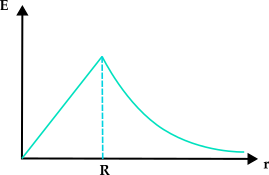
\includegraphics[width= 0.9\linewidth]{images/gsphera}
  \captionof{figure}{Intensit\`a del campo elettrico}
\end{minipage}%
\hspace{0.8cm}
\begin{minipage}{0.4\textwidth}
  \centering
  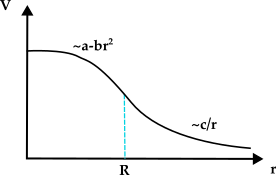
\includegraphics[width=0.9\linewidth]{images/potent}
  \captionof{figure}{Potenziale Elettrostatico}
\end{minipage}
\end{figure}
Notare che quando si fissa un punto di riferimento come $P_0 = + \infty$ tutti i cammini partono tutti da questo punto e dunque termini precedentemente calcolati per distanze pi\`u brevi compaiono in quelle pi\`u lunghe, come nel caso della misurazione del potenziale all'interno della sfera.
\subsection{Il Gradiente}

Consideriamo un generico campo scalare (funzione scalare) $\phi : \mathbb{R}^n \to \mathbb{R} $. Date le coordinate cartesiane $x_i $ per i =1,...,n, il gradiente di $\phi$ \`e dato da 
\begin{equation*}
	\nabla \phi = \left [ \frac{\partial \phi}{\partial x_1},...,\frac{\partial \phi}{\partial x_n} \right ] 
\end{equation*}
Differenziare un campo scalare ci porta ad avere un campo vettoriale. La possibilit\`a di poter definire il gradiente di una funzione scalare ci permette di definire il differenziale di $\phi$, ovvero
\begin{equation*}
	d\phi = \sum_{i} \frac{\partial \phi}{\partial x_i}dx_i = \nabla \phi \cdot d\bold{s}
\end{equation*}
che definisce la variazione di $\phi$ rispetto ad uno spostamento $d\bold{s} = [dx_1,...,dx_n]^T$. Tramite il gradiente di $\phi$ possiamo identificare la direzione e verso di massima crescita
\begin{equation*}
	df = ||\nabla \phi||\;||d\bold{s}|| \cos \theta 
\end{equation*}
e dunque $df$ \`e massimo quando $\nabla \phi$ \`e parallelo allo spostamento $d\bold{s}$.
\\
\noindent Nella sezione precedente abbiamo definito il potenziale elettrostatico che \`e una funzione scalare, se consideriamo una sua variazione infinitesima avremo che
\begin{equation*}
	dV = - \bold{E} \cdot d\bold{s} \iff dV = \nabla V \cdot d\bold{s} 
\end{equation*}
e quindi si ha che $\bold{E} = - \nabla V$, ovvero il campo elettrico \`e proporzionale e contrario al potenziale. Se moltiplichiamo tuto per una carica $q_0$ si ha che 
\begin{equation*}
	\bold{F}_e = - \nabla U_e
\end{equation*}
che \`e il risultato che ci aspettiamo di ottenere per una forza di natura conservativa.
\\
\noindent Si noti che fino a questo punto si \`e data una definizione del gradiente dipendente dalle coordinate cartesiane, ma esso pu\`o essere espresso rispetto ad altri sistemi di coordinate.
\\

\noindent Una conseguenza importante per le forze conservative \`e che dato un potenziale V(x,y,z), essendo una funzione scalare \`e possibile definirne le curve di livello, ed essendo $\bold{E} = - \nabla V$ si avr\`a che il campo elettrico in tutti i punti dello spazio in cui \`e definito \`e ortogonale a tali curve.
\subsubsection{Esempio - Carica Puntiforme}

\begin{wrapfigure}{r}{0.5\textwidth}
  \begin{center}
    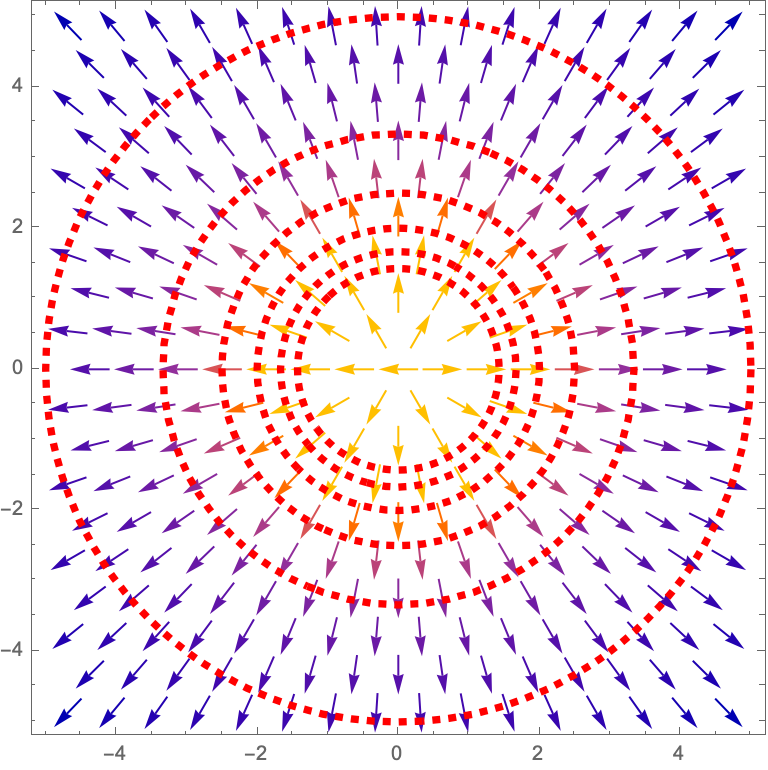
\includegraphics[width=0.4\textwidth]{images/contour}
  \end{center}
\end{wrapfigure}
Rispetto ad un sistema di coordinate cartesiane e prendendo $P_0 = + \infty$ come riferimento di misura si ha che il potenziale per una carica puntiforme posta nell'origine del sistema \`e dato da


\begin{equation*}
	V(x,y) = \frac{Q}{4 \pi \varepsilon_0} \frac{1}{\sqrt{x^2+y^2}}
\end{equation*}
 

\vspace{0.4cm}
\noindent calcolando le sue curve di livello avremo in figura che il campo elettrico $\bold{E}$ \`e ortogonale ad esse come in figura (circonferenza tratteggiate in rosso).
\newpage

\begin{lstlisting}{language = Mathematica}
Mathematica Snippets

V[x_, y_, q_] := (1/Sqrt[x^2 + y^2])
E1x[q_, x_, y_, x0_, y0_] := ((x - x0)/((x - x0)^2 + (y - y0)^2)^(1.5))
E1y[q_, x_, y_, x0_, y0_] := ((y - y0)/((x - x0)^2 + (y - y0)^2)^(1.5))

Show[VectorPlot[{E1x[Q, x, y, 0, 0], E1y[Q, x, y, 0, 0]}, {x, -5, 
   5}, {y, -5, 5}],
 ContourPlot[V[x, y, Q] , {x, -5, 5}, {y, -5, 5}, 
  ContourStyle -> Directive[Red, Dashed, Thickness[0.01]], 
  ContourShading -> None]]
\end{lstlisting}

\subsubsection{Esempio - Oscillatore Armonico}

\begin{wrapfigure}{r}{0.5\textwidth}
  \begin{center}
    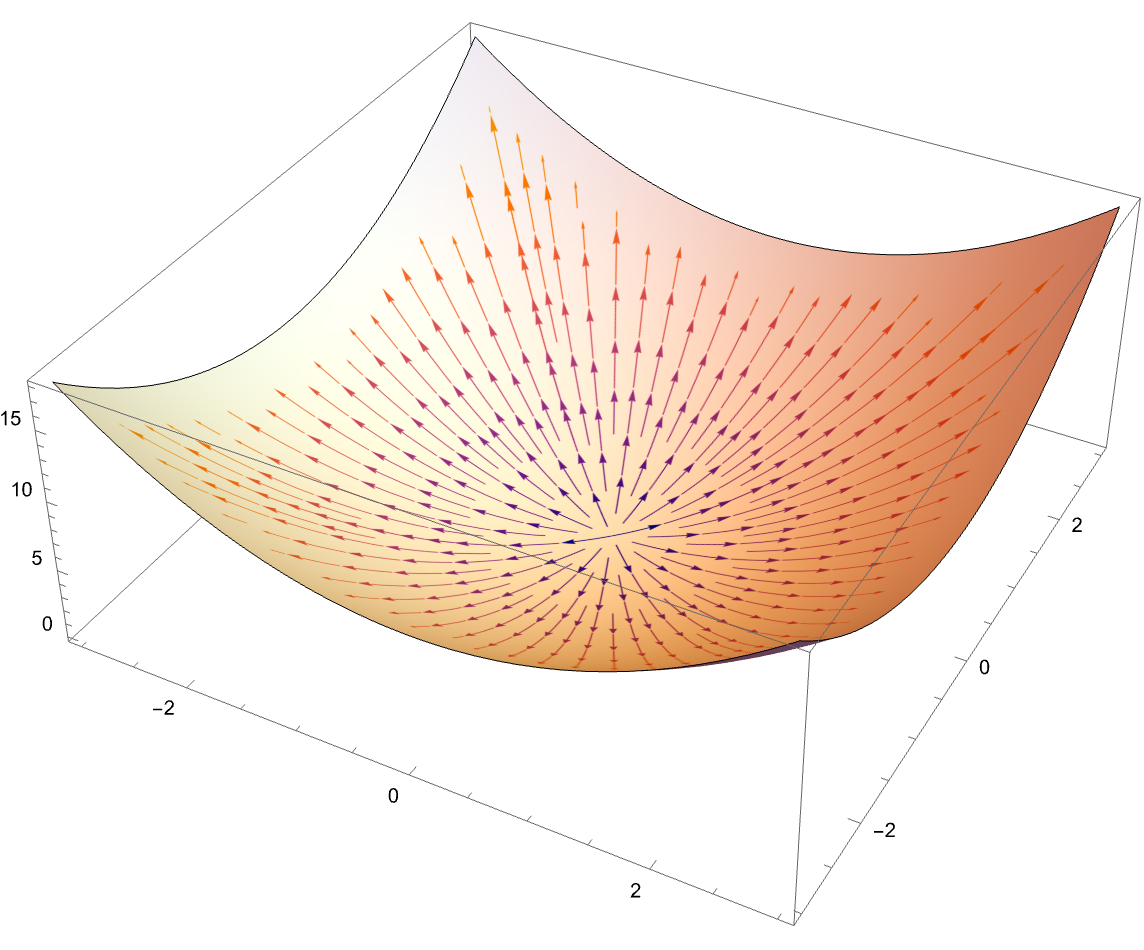
\includegraphics[width=0.5\textwidth]{images/harmonic}
  \end{center}
\end{wrapfigure}
Consideriamo una particella sottoposta ad una forza elastica vincolata a muoversi in una sola direzione. Ipotizziamo che non sia presenti attriti, dunque l'energia del sistema sar\`a data dalla funzione 
\begin{equation*}
	E(x,y) = \frac{1}{2}my^2 + \frac{1}{2}kx^2
\end{equation*}
rispettivamente il gradiente sar\`a un vettore della forma
\begin{equation*}
	\nabla E = \left [ \begin{array}{c}
		kx \\
		my
	\end{array} \right ]
\end{equation*}
e sar\`a tangente alla superficie data da E(x,y), come in figura.

\begin{lstlisting}
Mathematica Snippets 
	
Plot3D[(x^2 + y^2), {x, -3, 3}, {y, -3, 3}, 
 PlotStyle -> 
  Texture[StreamPlot[
    Evaluate[D[(x^2 + y^2), {{x, y}}]], {x, -3, 3}, {y, -3, 3}, 
    Frame -> None, ImageSize -> Large]], Mesh -> None, 
 ImageSize -> Large, PlotPoints -> 35]
\end{lstlisting}
\subsection{Potenziale per una distribuzione di cariche }

I risultati ottenuti nel paragrafo sul potenziale elettrostatico sono facilmente estendibili al caso in cui un campo elettrostatico \`e dato dalla distribuzione di pi\`u cariche puntiformi $q_1,...,q_n$, per farlo \`e sufficiente utilizzare il principio di sovrapposizione.
\\
Se consideriamo una carica sonda $q_0$ il lavoro compiuto per spostare la carica all'interno dell campo elettrostatico generato dalla distribuzione di cariche \`e dato da 
\begin{equation*}
	W =\int_{A}^{B} \bold{F} \cdot d\bold{s} = q_0 \int_{A}^{B} \bold{E} \cdot d\bold{s}
\end{equation*}
dato che il campo complessivo \`e dato da $\bold{E} = \sum_{i} \bold{E}_i$ dove $\bold{E}_i$ \`e il campo generato dalle singole cariche, dunque il potenziale assume la forma
\begin{equation*}
	\int_{A}^{B}\bold{E} \cdot d \bold{s} = \sum_{i}\int_{A}^{B} \bold{E}_i \cdot d\bold{s} = \sum_{i} \int _{A}^{B} \frac{q_i}{4 \pi \varepsilon_0 r_i^2} \; \hat{\mu}_i \cdot d\bold{s}
\end{equation*}
e quindi la differenza di potenziale \`e data d a
\begin{equation*}
	V(A) - V(B) = \sum_{i}\frac{q_i}{4 \pi \varepsilon_0 r_{A,i}^2} - \sum_{i}\frac{q_i}{4 \pi \varepsilon_0 r_{B,i}^2} 
\end{equation*}
Posto V(B) = 0 per $B = \infty$ si ha che 
\begin{equation}
	V(r) = \int_{P}^{\infty} \bold{E}  \cdot d \bold{s} = \sum_{i}\frac{q_i}{4 \pi \varepsilon_0 r_{i}^2}
\end{equation}
Tale risultato indica che il potenziale elettrostatico generato da un sistema di cariche puntiformi \`e uguale alla somma dei potenziali generati singolarmente dalle cariche. Possiamo estende il risultato per distribuzioni di carica continue 
\begin{equation}
	\begin{aligned}
		& V(r) = \frac{1}{4 \pi \varepsilon_0}\int_{C} ds \; \frac{\lambda(r)}{|r-r'|} & \\[0.5cm]
		& V(r) = \frac{1}{4 \pi \varepsilon_0} \int_{S} d\Sigma \; \frac{\sigma (r)}{|r-r'|} & \\[0.5cm]
		& V(r) = \frac{1}{4 \pi \varepsilon_0} \int_{V}dV \;  \frac{\rho(r)}{|r-r'|} 
	\end{aligned}
\end{equation}
Il potenziale elettrostatico risulta essere una funzione del punto, continua e derivabile, che pu\`o essere calcolabile una volta conosciuta la distribuzione delle cariche sorgente, indipendentemente dalla presenza di $q_0$. Infatti ci si rivolge ad esso anche come campo scalare. A differenza del campo vettoriale ci\`o che \`e significativo non \`e il valore che un potenziale assume in un punto, ma la sua variazione rispetto ad un riferimento fissato.

\subsection{Energia Potenziale Elettrostatica}

 L'energia potenziale $U(\bold{r})$ di una particella $q_0$ immersa nel campo elettrostatico $\bold{E}$, \`e data dal lavoro compiuto per spostarla da infinito ad un certo punto P dello spazio

\begin{equation*}
	U(\bold{r}) = -	q_0\int_{\infty}^{P} \bold{E} \cdot d\bold{r} = q_0 \int_{\infty}^{P} \nabla \phi \cdot d\bold{r} = q_0 \; \phi(\bold{r})  
\end{equation*}
dove assumiamo che $\phi(\bold{r}) \to 0$ per $\bold{r} \to \infty$.
\\

Consideriamo una distribuzione di carica formata dal cariche $q_i$ con posizioni $r_i$ nello spazio . Il potenziale elettrostatico immagazzinato in questa configurazione coincide con il lavoro necessario ad assemblare la configurazione della distribuzione di carica discreta (questo \`e dovuto al fatto che se dovessimo rilasciare le cariche la loro energia cinetica sarebbe coincidente con il potenziale latente del sistema). Dunque quanto lavoro \`e necessario per assemblare la configurazione della distribuzione di carica ?
\\

Fissiamo la prima carica nello spazio in $\bold{r_1}$. Il lavoro $W_1 =0$ dato che non \`e presente campo elettrostatico, poich\`e una carica non esercita forza su se stessa. Per spostare una seconda carica \`e necessario un lavoro di 
\begin{equation*}
	W_2 = \frac{q_1q_2}{4 \pi \varepsilon_0} \frac{1}{|\bold{r_1} - \bold{r_2}|}
\end{equation*}
Notare che se le due cariche hanno lo stesso segno $q_1q_2 > 0$ e dunque $W_2 > 0$, e dunque bisogna immettere lavoro nel sistema affinch\`e queste si avvicinino. Se $q_1q_2 < 0$ allora $W_2 < 0$ e quindi le particelle si avvicinano per mutua attrazione.
\\
Se ora avviciniamo una terza carica questa si dovr\`a spostare all'interno del campo elettrico generato dalle cariche $q_1$ e $q_2$ e dunque il lavoro necessario \`e 
\begin{equation*}
	W_3 = \frac{q_3}{4 \pi \varepsilon_0} \left [  \frac{q_2}{|\bold{r_2} - \bold{r_3}|} + \frac{q_1}{|\bold{r_1}-\bold{r_3}}\right ] 
\end{equation*}
e cos\`i via aggiungendo altre particelle. Il lavoro complessivo per assemblare la distribuzione di carica \`e data dall'energia potenziale immagazzinata nel sistema.
\begin{equation}
	U = \sum_{i=1}^NW_i = \frac{1}{2}\frac{1}{4 \pi \varepsilon_0}\sum_{i}\sum_{i\neq j} \frac{q_iq_j}{|\bold{r_i}-\bold{r_j}|}
\end{equation}
Se vogliamo misurare il potenziale nel punto $\bold{r_i}$ dovuto alle cariche $q_j,\;j\neq i$ si ha che
\begin{equation*}
	\phi(\bold{r_i}) = \frac{1}{4 \pi \varepsilon_0} \sum_{j \neq i} \frac{q_j}{|\bold{r_i}-\bold{r_j}|}
\end{equation*} 
e dunque possiamo riscrivere l'energia potenziale come 
\begin{equation}
	U = \frac{1}{2}\sum_{i=1}^Nq_i \phi(\bold{r_i})
\end{equation}
che rappresenta l'energia potenziale per una distribuzione discreta di cariche. Possiamo generalizzare tale risultato alle distribuzioni continue $\rho(\bold{r})$ definite una regione chiusa dello spazio. L'energia associata a una distribuzione continua \`e data da 
\begin{equation}
	U = \frac{1}{2} \int_V dV \; \rho(\bold{r})\phi(\bold{r})
\end{equation}
Ritorneremo successivamente su questa equazione quando introdurremo l'operatore di divergenza per un campo vettoriale.

\subsection{Esempi ed Esercizi}

\subsubsection{Potenziale di una distribuzione di carica superficiale a simmetria sferica}

Data una densit\`a di carica areica $\sigma$ costante distribuita su una sfera di raggio R, vogliamo determinare il potenziale $\phi(r)$ ad una generica distanza r da essa.

\newpage

\begin{figure}[!ht]
\vspace{0.1in}
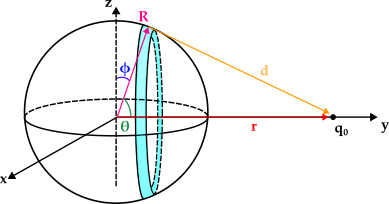
\includegraphics[width =10cm]{images/ringsym}	
\centering
\vspace{0.2in}
\end{figure}
Utilizzando il teorema di Carnot abbiamo che la distanza d data dalla diagonale in figura pu\`o essere espressa come 
\begin{equation*}
	d = \left [ R^2+r^2 -2rRcos\theta \right ]^{1/2} = ||\bold{R} -\bold{r}||
\end{equation*}
applicando l'espressione del potenziale per una distribuzione di carica continua si ha che 

\begin{equation*}
\begin{aligned}
	 & \phi(r) = \frac{1}{4 \pi \varepsilon_0} \int_{A} d\Sigma \; \frac{\sigma }{d} = \frac{1}{4 \pi \varepsilon_0} \int_{0}^{2\pi}d \varphi \int_{0}^{\pi}d\theta \; \frac{\sigma R^2 \sin\theta }{d} =  \frac{2\pi \sigma R^2}{4\pi \varepsilon_0} \int_{0}^{\pi}d\theta \; \frac{\sin \theta}{d} =  \\[0.5cm]
	& = \frac{Q}{8 \pi \varepsilon_0} \frac{1}{Rr} \left [(R^2+r^2 - 2rR \cos \theta)^{1/2} \right ]_{0}^{\pi} = \\[0.5cm]
	&  = \frac{Q}{8 \pi \varepsilon_0} \frac{1}{Rr} \left [(R^2+r^2+2rR)^{1/2} - (R^2+r^2-2rR)^{1/2} \right ] = \\[0.5cm]
	& = \frac{Q}{8 \pi \varepsilon_0} \frac{1}{Rr} \left [(R+r)-|R-r| \right ] 
\end{aligned}
\end{equation*}
\begin{wrapfigure}{r}{0.4\textwidth}
\vspace{-1.7cm}
  \begin{center}
    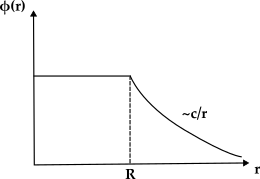
\includegraphics[width=0.4\textwidth]{images/chargesurf}
  \end{center}
\end{wrapfigure}
Per $Q = 4\pi R^2 \sigma $ (Carica di un anello) il potenziale \`e dato da
\begin{equation*}
	\phi(r) = 
	\left \{ \begin{array}{l}
		 \frac{Q}{4 \pi \varepsilon_0} \frac{1}{r} \quad r >R \\
		 \frac{Q}{4 \pi \varepsilon_0} \frac{1}{R} \quad r < R
		 \end{array}\right.
\end{equation*}
Il potenziale interno \`e costante e pari al potenziale della superficie.

\subsubsection{Potenziale per una distribuzione di carica lineica infinita}

\begin{wrapfigure}{r}{0.4\textwidth}
  \begin{center}
    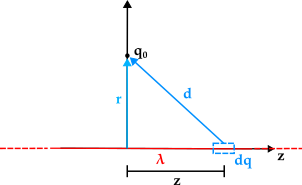
\includegraphics[width=0.4\textwidth]{images/lineinf}
  \end{center}
\end{wrapfigure}

Calcoliamo il potenziale elettrostatico per un filo di estensione infinita e carica $\lambda $ parallelo alla direzione $\hat{\bold{z}}$. Utilizzando la definizione di potenziale per una distribuzione di carica infinita 
\begin{equation*}
	\phi(r) = \frac{1}{4 \pi \varepsilon_0} \int_{-\infty}^{+\infty} dz \; \frac{\lambda}{d} = \frac{\lambda }{4 \pi \varepsilon_0} \int_{-\infty}^{+\infty} \frac{dz}{[z^2+r^2]^{1/2}}
\end{equation*}
nel calcolo si ha un problema in quanto 
\begin{equation*}
	\phi(r) \simeq \int \frac{1}{r}
\end{equation*}
e dunque il potenziale \`e divergente ad infinito. Per evitare questo problema calcoliamo l'integrale su un intervallo chiuso $[-L,L]$, con $L >> r$.
\begin{equation*}
	\phi(r) = \frac{1}{4 \pi \varepsilon_0} \int_{-L}^{L}dz \; \frac{\lambda}{[r^2+z^2]^{1/2}} = \frac{\lambda}{4 \pi \varepsilon_0} \ln \left[ \frac{(1+  r^2/L^2)^{1/2}+1}{(1+r^2/L^2)^{1/2} -1}\right ]
\end{equation*}
dato che $L >> r$ possiamo sviluppare con Taylor rispetto a $\frac{r^2}{L^2}$
\begin{equation*}
	\begin{aligned}
		& \phi(r) = \frac{\lambda}{4 \pi \varepsilon_0} \ln \left [ \frac{4L^2+r^2}{r^2} \right ] \simeq \frac{\lambda}{4 \pi \varepsilon_0} \ln \left[\frac{2L}{r} \right ]^2 = \frac{\lambda}{2 \pi \varepsilon_0} \ln \left[\frac{2L}{r}\right ] = \\[0.5cm]
		& = \frac{\lambda}{2 \pi \varepsilon_0} \left [ \ln \left ( \frac{1}{r} \right ) + \ln(2L)\right] = \frac{\lambda}{2 \pi \varepsilon_0} \ln \left ( \frac{1}{r} \right) + \text{cost} 
	\end{aligned}
\end{equation*}
in questo modo riusciamo a mettere a zero il potenziale per $r \to \infty$.
Utilizzando la relazione tra campo elettrostatico e gradiente del potenziale abbiamo che 
\begin{equation*}
	\bold{E} = - \frac{\partial \phi}{\partial r} \; \hat{\mu}_{r} = \frac{\lambda}{2 \pi \varepsilon_0} \frac{1}{r} \;\hat{\mu}_{r}
\end{equation*}
ottenendo il campo per una distribuzione di carica lineare e con estensione infinita.
\newpage

\subsubsection{Potenziale per una distribuzione di carica sulla superficie di un disco}

\begin{wrapfigure}{r}{0.4\textwidth}
\vspace{-0.3cm}
  \begin{center}
    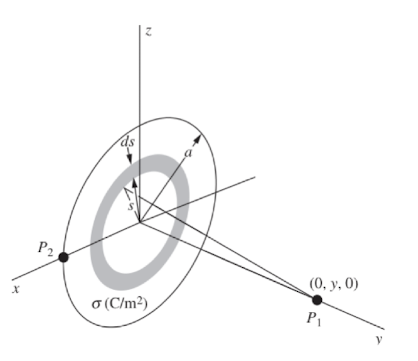
\includegraphics[width=0.4\textwidth]{images/disco}
  \end{center}
\end{wrapfigure}

Data una distribuzione di carica superficiale $\sigma$ per un disco di raggio R, vogliamo determinare il potenziale elettrostatico in funzione della posizione. Avremo che presa una distribuzione di carica infinitesima circolare con $dQ = 2 \sigma \pi rdr$, l'espressione per una distribuzione di carica continua del potenziale \`e data da
\begin{equation*}
\begin{aligned}
	& \phi(0,y,0) = \frac{1}{4 \pi \varepsilon_0}\int_{0}^{R} \frac{2 \pi \sigma rdr}{[r^2 + y^2]^{1/2}}\\[0.5cm] & = \frac{\sigma}{2 \varepsilon} \int_{0}^{R}dr \; \frac{r}{[r^2+y^2]^{1/2}} = \frac{\sigma}{2 \varepsilon} \left [\sqrt{r^2+y^2}\right ]_{0}^{R} = & \\[0.5cm]
	& = \frac{\sigma}{2 \varepsilon_0}\left[ \sqrt{R^2+y^2} - |y| \right ]
\end{aligned}
\end{equation*}
Dato che \`e presente un modulo all'interno dell'espressione del potenziale si ha che, questo assume valori diversi lungo y per $y>0$ o $y<0$.

\begin{equation*}
	\phi(y) = \left \{ \begin{array}{l}
		\frac{\sigma }{2 \varepsilon_0} \left [ \sqrt{R^2+y^2} - y \right ] \quad y > 0 \\[0.5cm]
		\frac{\sigma}{2 \varepsilon_0} \left [ \sqrt{R^2+y^2} + y \right ] \quad y < 0
	\end{array}\right.
\end{equation*}
\\

\noindent Il potenziale \`e continuo in $y = 0$ a differenza del campo elettrostatico che presenta un punto di discontinuit\`a a cuspide.
\begin{equation*}
	\bold{E} = - \nabla \phi = -\frac{d \phi}{dy}\Big |_{y=0} = \left \{ \begin{array}{l}
		\frac{\sigma}{2 \varepsilon_0} \quad y>0 \\
		-\frac{\sigma}{2 \varepsilon_0} \quad y < 0
	\end{array}\right.
\end{equation*}
\begin{remark}	
\end{remark}

\begin{itemize}
	\item Per $y \to 0^{\pm}  $ si ha che il potenziale del disco coincide con quello di un piano infinito.
	\item Nel limite in cui $y >> R$, il comportamento del potenziale \`e uguale a quello di una carica puntiforme.
	\begin{equation*}
		\phi(y) = \frac{\sigma}{2 \varepsilon_0}y \left [ \left ( 1+ \frac{R^2}{y^2}\right)^{1/2} - 1\right ] \simeq_{\text{Taylor}} \frac{\sigma R^2}{4  \varepsilon_0} \frac{1}{y}
	\end{equation*}
\end{itemize}
e dunque il campo scalare ha una discontinuit\`a in $y =0 $.
 
\begin{figure}[!ht]
\vspace{0.1in}
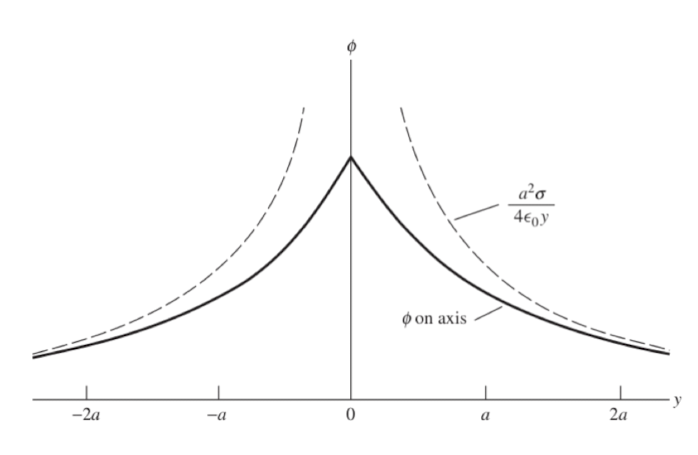
\includegraphics[width = 10cm]{images/disco_discont.png}	
\centering
\vspace{0.1in}
\end{figure}

\section{Divergenza di un  Campo Vettoriale}

La divergenza di un campo vettoriale ci permette di esprimere la legge di Gauss in forma differenziale, legando le propriet\`a locali del campo elettrostatico alla distribuzione di carica. In sostanza consideriamo la variazione infinitesima del campo elettrostatico in un intorno di un punto dello spazio.
\\

\noindent Presa una regione di spazio V chiusa e al cui interno \`e contenuta della carica, abbiamo visto che questa fluisce attraverso la superficie data dal bordo $S = \partial V$ di S. Il flusso \`e dato dall'equazione
\begin{equation*}
	\phi(\bold{F}) = \int_{S} \bold{F} \cdot d\bold{A}
\end{equation*} 
Se immaginiamo di affettare la regione di spazio, otteniamo diverse sezioni $V_i$ attraverso cui parte del flusso passa attraverso, di conseguenza possiamo riscrivere il flusso totale come
\begin{equation*}
	\phi(\bold{F}) = \sum_{i=1}^N \int_{ S_i} \bold{F} \cdot d\bold{A}_i
\end{equation*}
ovvero la somma dei contributi delle singole regioni attraverso cui il campo passa attraverso. Per $N \to \infty$, ovvero aumentando i sezionamenti si ha che i rispettivi volumi $V \to 0$ e dunque ogni singolo contributo descrive un flusso locale.
\\

\noindent Il problema con questa definizione \`e che $\int_{S_i} \bold{F} \cdot d\bold{A}_i$ dipende dalla scelta del volume $V_i$ e dunque dalla scelta della superficie $S_i$ e dunque non si ha una buona misura del campo locale.
\\
Per esempio se prendiamo un volume $V_i$ se lo raddoppiamo o lo dimezziamo il risultato della misura del flusso aumenta e diminuisce (per $\bold{F}$ costante) e questo non ci permette di avere una buona stima di come sia cambiato il campo nelle regioni. Se $\bold{F}$ non \`e costante il problema \`e che riducendo il volume a 0 anche il flusso diventa nullo.
\\

Per dare una buona definizione locale di flusso consideriamo il suo valore medio rispetto al volume $V_i$
\begin{equation*}
	\langle \phi(\bold{F}) \rangle = \frac{1}{V}\int_{S_i} \bold{F} \cdot d \bold{A}_i
\end{equation*}
Tale equazione ci permette di definire la divergenza del campo $\bold{F}$ nel seguente modo
\begin{equation}
	\text{div}\bold{F} = \lim_{V_i \to 0} \frac{1}{V_i} \int_{S_i} \bold{F} \cdot d\bold{A}_i
\end{equation}
La divergenza di un vettore \`e una grandezza scalare che misura il flusso (locale) uscente da una superficie normalizzata al volume da essa racchiuso. Tale definizione ci rende la misura della divergenza del campo indipendente dalla geometria dei volumi.
\\

\noindent Uno dei risultati pi\`u importanti della teoria dei campi vettoriali \`e \textit{il teorema di divergenza di Gauss}, la cui espressione possiamo ottenere, considerando
\begin{equation}
	\int_{S}\bold{F} \cdot d\bold{A} = \lim\limits_{\substack{N \to +\infty \\[0.1cm] V_i \to 0}}\left [ \sum_{i=1}^N \frac{1}{V_i} \int_{S_i} \bold{F} \cdot d\bold{A}_i \right ] = \int_{V}\text{div}\bold{F} \; dV
\end{equation}

\begin{remark}
\end{remark}
\begin{itemize}
	\item Il teorema di Gauss \`e una propriet\`a matematica che vale per qualsiasi campo vettoriale.
	\item Il vettore $\bold{E}$ soddisfa una legge fisica (la legge di Gauss) che collega il flusso alla distribuzione di carica.
\end{itemize}	

\noindent Se consideriamo il campo elettrostatico $\bold{E}$ generato da una distribuzione di carica continua $\rho$ per la legge di Gauss abbiamo che
\begin{equation*}
	\phi(\bold{E})=\int_{S}\bold{E} \cdot d\bold{A} = \frac{1}{\varepsilon_0} \int_{V} \rho \; dV
\end{equation*}
per il flusso del campo possiamo applicare il teorema di divergenza di Gauss, in questo modo abbiamo che 
\begin{equation*}
	\int_{V} \text{div}\bold{E} \; dV = \frac{1}{\varepsilon_0} \int_{V} \rho \; dV
\end{equation*}
Dato che tale uguaglianza \`e soddisfatta per ogni volume e superficie, l'uguaglianza deve essere soddisfatta anche dai termini integrandi, definendo in questo modo \textit{la forma differenziale della legge di Gauss}.
\begin{equation}
	\text{div}\bold{E} = \frac{\rho}{\varepsilon_0} 
\end{equation}
Il ragionamento logico con cui si \`e ottenuta la divergenza di un campo fa s\`i che la definizione (1.20) non dipenda da un sistema di coordinate e quindi vale per tutti. Da un punto di vista applicativo per\`o risulta essere poco utile e quindi abbiamo bisogno di darne una seconda definizione pi\`u funzionale.

\subsection{Espressione della Divergenza in coordinate cartesiane}

Prendiamo un punto $\bold{x_0}$ dello spazio e consideriamolo come centro di un volume infinitesimo $dV=dxdydz$, data la presenza di un campo vettoriale $\bold{F}$ vogliamo determinare la divergenza localmente in coordinate cartesiane. Partendo dalla definizione di divergenza ed esplicitando il prodotto scalare dell'integrando si avr\`a che 
\begin{equation*}
 \text{div}\bold{F} =  \lim_{V \to 0} \frac{1}{V} \int_{S} \bold{F} \cdot d\bold{A} = \lim_{V \to 0 } \frac{1}{V} \left [ \int_{S} F_{x}\text{dydz} + \int_{S} F_y \text{dxdz} + \int_{S} F_z \text{dxdy}\right ]
	 \end{equation*}
utilizzando il teorema della media integrale per una delle facciate del cubo si ha per esempio che 
\begin{equation*}
	\int_{S_1}\bold{F}\cdot \bold{\hat{n}}(\text{dydz}) \simeq F_x(x_0+\frac{dx}{2},y,z)\Delta y \Delta z
\end{equation*}
in cui consideriamo la componente 'x' del campo valutata in un generico punto. 
 
\begin{figure}[ht]
\vspace{0.1in}
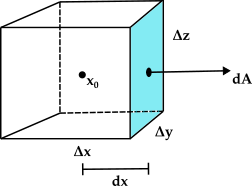
\includegraphics[width = 5cm]{images/cube}	
\centering
\vspace{0.1in}
\end{figure}
Possiamo reiterare lo stesso ragionamento per la faccia opposta, cambiando segno
\begin{equation*}
	-\int_{S_2}\bold{F}\cdot \bold{\hat{n}}(\text{dydz}) \simeq -F_x(x_0-\frac{dx}{2},y,z)\Delta y \Delta z
\end{equation*}
se vogliamo ottenere il contributo complessivo dato dall'addendo $\int_{S} F_{x}\text{dydz}$ dobbiamo considerare la superficie $S = S_1+S_2$ e quindi si ha che 
\begin{equation*}
	\int_{S} F_{x}\text{dydz} \simeq F_x(x_0+\frac{dx}{2},y,z)\Delta y \Delta z -F_x(x_0-\frac{dx}{2},y,z)\Delta y \Delta z
\end{equation*}
normalizzando rispetto al volume otteniamo l'equazione 
\begin{equation*}
	\frac{1}{V}\int_{S} F_{x}\text{dydz} \simeq \frac{F_x(x_0+\frac{dx}{2},y,z)-F_x(x_0-\frac{dx}{2},y,z)}{\Delta x}
\end{equation*}
e prendendo il limite per $V \to 0$ possiamo conclude che 
\begin{equation*}
	\lim_{V \to 0} \frac{1}{V}\int_{S} F_{x}\text{dydz} \simeq \lim_{\Delta x  \to 0} \frac{1}{V}\int_{S} F_{x}\text{dydz} \simeq \frac{F_x(x_0+\frac{dx}{2},y,z)-F_x(x_0-\frac{dx}{2},y,z)}{\Delta x} = \frac{\partial F_{x}}{\partial x }
\end{equation*}

Ripetendo i medesimi ragionamenti per gli addendi possiamo concludere che 
\begin{equation}
	\text{div}\bold{F} = \frac{\partial F_x}{\partial x} + \frac{\partial F_y}{\partial y} + \frac{\partial F_z}{\partial z}
\end{equation}
esprimendo la divergenza rispetto ad un sistema di coordinate cartesiane.
\\

\noindent Possiamo esprimere la divergenza utilizzando l'operatore gradiente 
\begin{equation*}
	\nabla = \frac{\partial }{\partial x_i}\bold{e}_i
\end{equation*}
che rappresenta sia un operatore che un vettore. Lo definiamo operatore perch\`e agisce sugli sugli spazi di funzione. Se facciamo agire l'operatore sul campo vettore $\bold{F}$ definito da una mappa
\begin{equation*}
	\bold{F} : \mathbb{R}^N \to \mathbb{R}^N
\end{equation*}
definiamo l'azione di $\nabla $ su $\bold{F}$ come il loro prodotto vettoriale 
\begin{equation}
	\text{div} \bold{F} = \nabla \cdot \bold{F} 
\end{equation}
in questo manteniamo la propriet\`a in cui la divergenza di un campo vettoriale deve restituire un campo scalare.
\\

\noindent Da un punto di vista fisico il segno della divergenza ci dice che se $\nabla \cdot \bold{F}>0$ localmente si ha un flusso netto uscente dal volume infinitesimo, viceversa per $\nabla \cdot \bold{F} < 0$ il flusso netto \`e localmente entrante nel volume.
\\

\noindent La forma della divergenza espressa rispetto all'operatore gradiente, ci permette di riscrivere la forma differenziale della legge di Gauss come
\begin{equation}
\boxed{
	\nabla \cdot \bold{E} = \frac{\rho}{\varepsilon_0}}
\end{equation}
questa espressione definisce una delle equazioni fondamentali dell'elettromagnetismo e prende il nome di \textit{prima equazione di Maxwell per l'elettrostatica}.


\subsection{Propriet\`a dell' operatore gradiente }

L'operatore gradiente \`e un operatore differenziale lineare, ovvero valgono le seguenti propriet\`a 
\begin{equation}
\begin{aligned}
\nabla(\alpha \phi+\psi) & =\alpha \nabla \phi+\nabla \psi \\
\nabla \cdot(\alpha \mathbf{F}+\mathbf{G}) & =\alpha \nabla \cdot \mathbf{F}+\nabla \cdot \mathbf{G}
\end{aligned}
\end{equation}
per ogni campo scalare $\phi$ e $\psi$, campo vettoriale $\bold{F}$ e $\bold{G}$ e costante $\alpha$.

Inoltre vale la propriet\`a di Leibniz, che \`e una generalizzazione della regola del prodotto, ovvero
\begin{equation}
\begin{aligned}
\nabla(\phi \psi) & =\phi \nabla \psi+\psi \nabla \phi \\
\nabla \cdot(\phi \mathbf{F}) & =(\nabla \phi) \cdot \mathbf{F}+\phi(\nabla \cdot \mathbf{F})
\end{aligned}
\end{equation} 
per $\phi,\psi$ campi scalari e $\bold{F}$ campo vettoriale.

\subsection{Esempi ed Esercizi}

\subsubsection{Campo elettrostatico di una lastra infinita}

\begin{wrapfigure}{r}{0.5\textwidth}
  \centering
  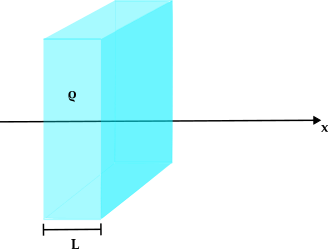
\includegraphics[width=0.5\textwidth]{images/lastra}
\end{wrapfigure}

Calcoliamo il campo elettrostatico per una lastra di superficie infita e spesso L, data una densit\`a di carica di volume $\rho$ uniforme. 
\\

\noindent Come fatto per gli esercizi precedenti per ragioni di simmetria sappiamo che il campo $E_z = E_y = 0$.
\\ Questa volta per\`o utilizziamo la forma differenziale dell'equazione di Gauss per calcolare il campo.

\begin{equation*}
	\nabla \cdot \bold{E} = \frac{\rho}{\varepsilon_0} \iff \frac{\partial E_x(x)}{\partial x} = \frac{\rho}{\varepsilon_0}
\end{equation*}
risolvendo l'equazione differenziale per quadrature si ha che 
\begin{equation*}
	E_x(x) = \frac{\rho}{\varepsilon_0}x + A
\end{equation*}
dove il termine A \`e la costante d'integrazione per un integrale indefinito.
\begin{remark}
Si noti che se consideriamo $\bold{E}(x) = \left ( \frac{\rho}{\varepsilon_0}x+A \right ) \hat{\mu}_{x}$	 e se applichiamo l'operatore gradiente al campo si ha che 
\begin{equation*}
	\nabla \cdot \bold{E} = \nabla \cdot \left ( \frac{\rho}{\varepsilon_0}x \hat{\mu}_{x}\right) + \nabla \cdot (A \hat{\mu}_x) = \frac{\rho}{\varepsilon_0} 
\end{equation*}
dunque il termine $\nabla \cdot (A \hat{\mu}_x) = 0$. In genere un campo vettoriale $\bold{F}$ \`e caratterizzato dalla divergenza a meno di un vettore a divergenza nulla. Che possiamo parafrasare pensato al fatto che esista una parte del campo che non contribuisce al flusso netto attraverso una superficie.
\end{remark}
Ritornando alla risoluzione del problema, abbiamo bisogno di definire delle condizioni al contorno che ci determinino il valore della costante A, per farlo osserviamo che se poniamo una carica esploratrice $q_0$ in $\bold{x} = 0$ (che coincide con il centro della lastra) avremo che la forza esercitata sulla carica \`e nulla per simmetria e dunque anche $\bold{E} = 0$. Risolvendo
\begin{equation*}
	0 =E_x(x=0) = \frac{\rho}{\varepsilon_0} \cdot 0 + A \Rightarrow A =0
\end{equation*}
In generale $A = \frac{\sigma}{2 \varepsilon_0}$, ovvero \`e dato da una distribuzione superficiale di carica.
Esternamente alla distribuzione di carica si ha che $\nabla \cdot \bold{E} = 0$ e quindi 
$ E_x = C$ \`e costante in tutte le regioni $|x| > \frac{L}{2}$. Per determinare il valore di C osserviamo che per $x = \pm \frac{L}{2}$ si ha che $E_x = \pm \frac{\rho L}{2\varepsilon_0} = C$
dato che il campo \`e una funzione continua. In conclusione troviamo che 
\begin{equation*}
	E_x(x) = \left \{ \begin{array}{l}
		\frac{\rho L}{2 \varepsilon_0} \quad x > \frac{L}{2}\\
		\frac{\rho }{\varepsilon_0}x \quad -\frac{L}{2} < x < \frac{L}{2}\\
		\frac{\rho L}{2 \varepsilon_0} \quad x < -\frac{L}{2}
	\end{array}\right.
\end{equation*} 

\section{Rotore di un campo vettoriale }
Analogamente a quanto fatto per la divergenza, costruiamo una grandezza locale legata ad un campo vettoriale $\bold{F}$ che traduca in termini locali la legge della di circuitazione di $\bold{F}$.
\\

\noindent Presa una regione di spazio definita da una volume V chiuso, consideriamo la sua superficie $S = \partial V$ che viene attraversata da un campo vettoriale $\bold{F}$ e ipotizziamo di definire su S un cammino chiuso C su cui vogliamo calcolare l'integrale di linea 
\begin{equation*}
	\oint_{C} \bold{F} \cdot d\bold{s} = \Gamma_{C}
\end{equation*}
Se spezziamo il cammino in due sotto cammini $C_1$ e $C_2$ possiamo riscrivere l'integrale precedente come 
\begin{equation*}
	\oint_{C } \bold{F} \cdot d \bold{s} = \oint_{C_1} \bold{F} \cdot d\bold{s} \;+\; \oint_{C_2}\bold{F} \cdot d\bold{s}
\end{equation*}
reiterando il procedimento di suddivisione si ha che 
\begin{equation*}
	\oint_{C} \bold{F} \cdot d \bold{s} = \sum_{i=1}^N \oint_{C_i} \bold{F} \cdot d \bold{s}
\end{equation*}
una condizione necessaria \`e che i contributi sulle linee esterne, siano percorsi in versi opposti in modo da elidersi.

\begin{wrapfigure}{l}{0.4\textwidth}
    \centering
    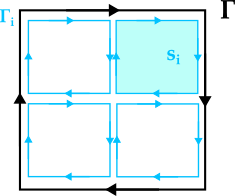
\includegraphics[width=0.38\textwidth]{images/rot} % sostituisci con il nome dell'immagine
\end{wrapfigure}
La definizione $\oint_{C_i} \bold{F} \cdot d \bold{s}$ ha dei problemi nella sua definizione di circuitazione, in quanto l'integrale di linea aumenta all'aumentare della dimensione del circuito nel caso in cui $\bold{F}$ sia costante. Inoltre facendo tendere a zero la superficie $S_i$ racchiusa dal cammino, nel limite puntiforme l'integrale si annulla. Per correggere questa dipendenza dalla geometria del cammino, normalizziamo il circuito rispetto alla superficie $S_i$ che racchiude.
\begin{equation*}
	\frac{1}{S_i} \oint_{C_i} \bold{F} \cdot d\bold{s}
\end{equation*} 
in questo modo si ottiene una buona definizione locale dell'integrale di linea. Tuttavia anche se si perde la dipendenza geometrica rimane la dipendenza dal senso di percorrenza del cammino.
Dato che l'equazione non dipende da una cammino $C_i$ che racchiude una superficie $S_i$ in particolare il segno dell'equazione dipende da come si \`e scelto di suddividere il percorso, mano a mano che si rendono infinitesime le superfici, di conseguenza il passaggio al limite rifletter\`a questa propriet\`a.  Per poter tener conto dell'informazione direzionale introduciamo il vettore $\bold{\hat{n}}$ ortogonale alla superficie infinitesima. 

\begin{wrapfigure}{l}{0.4\textwidth}
    \centering
    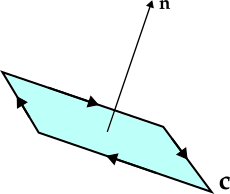
\includegraphics[width=0.38\textwidth]{images/direc} % sostituisci con il nome dell'immagine
\end{wrapfigure}
In questo modo definiamo rotore di un campo vettoriale $\bold{F}$ la grandezza.
\begin{equation}
	\text{rot}\bold{F} \cdot \ \bold{\hat{n}} = \lim_{S_i \to 0} \frac{1}{S_i} \oint_{C_i} \bold{F} \cdot d \bold{s}
\end{equation}
Possiamo domandarci come l'informazione locale che ci viene data dal rotore di un campo si leghi all'integrale di linea del circuito di partenza C da cui siamo partiti. Per rispondere a questa domanda sommiamo tutti i contributi dati che concorrono a formare $C = \sum_i C_i$ 
\begin{equation*}
	\oint_{C} \bold{F} \cdot d \bold{s} = \lim_{\substack{N \to \infty \\[0.2cm] S_i \to 0}} \sum_{i=1}^N \left [\frac{1}{S_i} \oint_{C_i} \bold{F} \cdot d \bold{s} \right ] S_i = \int_S \text{rot}\bold{F}\cdot\bold{\hat{n}}dA = \phi(\text{rot}\bold{F})
\end{equation*}
il risultato
\begin{equation}
	\oint_{C} \bold{F} \cdot d \bold{s} = \int_S \text{rot}\bold{F}\cdot\bold{\hat{n}}dA 
\end{equation}
prende il nome di \textit{teorema di Stokes}. Questo teorema ci dice che la circuitazione di un campo $\bold{F}$ \`e uguale al flusso del rotore di $\bold{F}$ attraverso una qualunque superficie aperta il cui bordo \`e definito dal circuito.

\subsection{Espressione del rotore in coordinate cartesiane}

L'espressione del rotore (1.27) risulta essere poco utile nell'applicazione non dipendendo esplicitamente da un sistema di coordinate. In questo paragrafo esprimiamo il rotore in funzione delle coordinate cartesiane, per farlo prendiamo un punto $\bold{x}_0$ come centro del circuito della faccia giacente nel piano (x,y) di un cubo di volume $dV$ infinitesimo. Possiamo riscrivere l'espressione (1.27) esplicitandone l'integrando di destra 
\begin{equation*}
	\text{rot} \bold{F} \cdot \hat{\bold{n}} = \lim_{S \to 0} \frac{1}{S} \left [ \oint_{C} (F_{y}\text{dy}+F_z\text{dz}) \; +\; \oint_{C} (F_x\text{dx}+F_z\text{dz}) \; + \; \oint_{C}(F_x\text{dz} + F_y\text{dy})\right ]
\end{equation*}
Prendiamo in esame l'ultimo addendo dell'espressione, questo esprime l'integrale di linea di un cammino C giacente nel piano (x,y). 
\newpage

 
\begin{figure}[!ht]
    \begin{minipage}{0.4\textwidth}
        \centering
        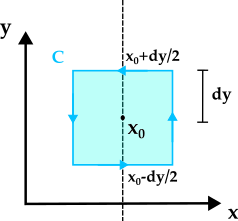
\includegraphics[width=\linewidth]{images/rotar}
    \end{minipage}
   \hspace{2cm}
    \begin{minipage}{0.4\textwidth}
        \centering
        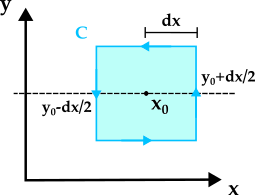
\includegraphics[width=\linewidth]{images/rotar1}
    \end{minipage}
\end{figure}
Utilizzando il teorema della media integrale possiamo esprimerlo come 
\begin{equation*}
	\int_{C_1} F_x dx \simeq F_x(x,y_0-\frac{dy}{2},z)\Delta x  
\end{equation*}
per il cammino $C_1$ inferiore parallelo ad x, mentre per il cammino $C_2$ superiore e parallelo ad x si ha
\begin{equation*}
	-\int_{C_2}F_xdx \simeq F_x(x,y_0+ \frac{dy}{2},z)\Delta x
\end{equation*} 
di conseguenza possiamo riscrivere 
\begin{equation*}
	\frac{1}{\Delta x \Delta y}\int_{C_1+C_2}F_x dx \simeq - \frac{F_x(x,y_0+\frac{dy}{2},z) - F_x(x,y_0-\frac{dy}{2},z)}{\Delta y}
\end{equation*}
facendo il limite per $S \to 0$ si ha che
\begin{equation*}
	\lim_{\Delta x \Delta y \to 0 } \frac{1}{\Delta x \Delta y}\int_{C_1+C_2}F_x dx \simeq \lim_{\Delta y \to 0} - \frac{F_x(x,y_0+\frac{dy}{2},z) - F_x(x,y_0-\frac{dy}{2},z)}{\Delta y} =-\frac{\partial F_x}{\partial y}
\end{equation*}	

Ripentendo lo stesso procedimento per la componente y del campo vettoriale si ha che 
\begin{equation*}
	\lim_{\Delta x \Delta y \to 0} \frac{1}{\Delta x \Delta y} \int_{C_3+C_4}F_y \text{dy} = \lim_{\Delta x \to 0}\frac{F_y(x_0+\frac{dx}{2},y,z) - F_y(x_0-\frac{dx}{2},y,z)}{\Delta x} = \frac{\partial F_y}{\partial x}
\end{equation*}
dunque possiamo concludere che la componente del rotore lungo $\hat{z}$ e dunque ortogonale al circuito \`e data da 
\begin{equation}
	(\text{rot}\bold{F})_z = \oint_{C} (F_x\text{dx}+F_y\text{dy}) = \frac{\partial F_y}{\partial x}-\frac{\partial F_x}{\partial y} 
\end{equation}
 Ripetendo gli stessi procedimenti per le altre direzione del vettore rotore possiamo concludere che 
 \begin{equation*}
 	\text{rot}\bold{F} = \left [ \frac{\partial F_z}{\partial y} - \frac{\partial F_y}{\partial z} \right] \hat{\mu}_{x} + \left [ \frac{\partial F_x}{\partial z} - \frac{\partial F_z}{\partial x}\right] \hat{\mu}_{y} + \left[ \frac{\partial F_y}{\partial x}-\frac{\partial F_x}{\partial y}\right]\hat{\mu}_{z}
 \end{equation*}
\\
\noindent A differenza dell'operazione di gradiente e di divergenza che possono essere definiti su tutto $\mathbb{R}^N$, l'operazione di rotore \`e definita solo per spazi vettoriale in $\mathbb{R}^3$. Possiamo definire l'operazione di rotore utilizzando l'operatore nabla come fatto per la divergenza. In questo avremo che il rotore di un campo $\bold{F} : \mathbb{R}^3 \to \mathbb{R}^3$ \`e esprimibile come 
\begin{equation*}
	\text{rot}\bold{F} = \nabla \times \bold{F}
\end{equation*}  
che definisce ancora un campo vettoriale. Inoltre il rotore pu\`o anche essere espresso come determinante 
\begin{equation*}
	\nabla \times \bold{F} = \text{det}\left [\begin{array}{ccc}
		\bold{e}_1 & \bold{e}_2 & \bold{e}_3 \\
		\frac{\partial}{\partial x} & \frac{\partial }{\partial y} & \frac{\partial}{\partial z}\\
		F_1 & F_2 & F_3
	\end{array}\right ]
\end{equation*}
\noindent Riassumendo abbiamo che la divergenza di un campo vettoriale $\nabla \cdot \bold{F}$ misura il flusso netto del campo attraverso una superficie, mentre il rotore $\nabla \times \bold{F}$ misura la sua rotazione. L'operazione di rotore \`e di fondamentale importanza per determinare se un campo vettoriale pu\`o essere un campo elettrostatico.

\subsection{Propriet\`a del rotore}

Il rotore \`e un operatore differenziale lineare e dunque soddisfa la condizione 
\begin{equation*}
	\nabla \times (\alpha \bold{F} + \bold{G}) = \alpha \nabla \times \bold{F} + \nabla \times \bold{G}
\end{equation*}
per ogni campo vettoriale $\bold{F}$ e $\bold{G}$ e costante $\alpha$. Inoltre gode della propriet\`a di Leibniz 
\begin{equation*}
\begin{aligned}
	& \nabla \times (\phi \bold{F}) = (\nabla \phi) \times \bold{F} + \phi(\nabla \times \bold{F}) \\ 
	& \nabla \cdot (\bold{F} \times \bold{G}) = (\nabla \times \bold{F}) \cdot \bold{G} - \bold{F} \cdot (\nabla \times \bold{G}) 
\end{aligned}
\end{equation*}
dove l'ordine in cui si posizione l'operatore $\nabla$ \`e fondamentale affinch\`e le uguaglianze siano verificate.
\\
Una propriet\`a importante \`e data dal fatto che se ipotizziamo di avere un campo vettoriale $\bold{F}$  conservativo che possiamo esprimere come il gradiente di un campo scalare $\phi$ e ne calcoliamo il rotore, avremo che 
\begin{equation*}
	\nabla \times (\nabla\phi) = 0
\end{equation*}
a patto che $\phi$ soddisfi l'identit\`a di Schwartz, ovvero che sia una funzione  le cui derivate parziali miste sono funzioni continue.

\subsection{Campi conservativi e irrotazionalit\`a}

Sappiamo che un campo vettoriale $\bold{F}$ conservativo pu\`o essere espresso come
\begin{equation*}
	\bold{F} = \nabla \phi
\end{equation*}
per un campo scalare $\phi$. Inoltre un campo vettoriale si dice \textit{irrotazionale} se $\nabla \times \bold{F} = 0$. Per un campo che possiede queste propriet\`a possiamo definire il seguente teorema.
\begin{theorem}
	Per un campo definito ovunque in $\mathbb{R}^3$, essere conservativo \`e equivalente ad essere irrotazionale.
	\begin{equation*}
		\nabla \times \bold{F} \iff \bold{F} = \nabla \phi
	\end{equation*}
\end{theorem}

questo risultano \`e importante in quanto se lo leghiamo al teorema di Stokes dove
\begin{equation*}
	\int_{S}(\nabla \times \bold{F})\cdot \hat{n} = \oint_{C} \bold{F} \cdot d\bold{s}
\end{equation*}
ci permette di concludere che 
\begin{equation*}
	\oint_{C} \bold{F} \cdot d\bold{s} = 0
\end{equation*}
In conclusione nel caso dell'elettrostatica possiamo concludere che un campo vettoriale \`e un campo elettrostatico se e solo se soddisfa il teorema (1.10.1).
\newpage


\section{Equazioni dell'elettrostatica}

\subsection{Operatore Laplaciano}

Il Laplaciano \`e un operatore differenziale del secondo ordine definito da 
\begin{equation*}
	\nabla^2 = \nabla \cdot \nabla = \sum_{i}\frac{\partial^2}{\partial x_i^2}
\end{equation*}
Per esempio su uno spazio vettoriale $\mathbb{R}^3$ il Laplaciano in coordinate cartesiane ha forma
\begin{equation*}
	\nabla^2 = \frac{\partial^2}{\partial x^2} + \frac{\partial^2}{\partial y^2 } + \frac{\partial^2}{\partial z^2}
\end{equation*}
L'operatore Lapalaciano \`e un operatore differenziale scalare, ovvero agisce su campi scalari $\phi$ e restituisce un altro campo scalare $\nabla^2\phi$. Similmente, se agisce componente per componente su un campo vettoriale $\bold{F}$, restituisce un campo vettoriale $\nabla^2\bold{F}$. Se utilizziamo la formula del triplo prodotto scalare si ha 
\begin{equation*}
	\nabla \times (\nabla \times \bold{F}) = \nabla(\nabla \cdot \bold{F} ) - \nabla^2 \bold{F}
\end{equation*}
da cui possiamo ottenere un espressione alternativa del Laplaciano
\begin{equation*}
	\nabla^2 \bold{F} = \nabla(\nabla \cdot \bold{F}) - \nabla \times (\nabla \times \bold{F})
\end{equation*}
\subsection{Equazione di Poisson}

Consideriamo il campo elettrostatico $\bold{E}$ abbiamo visto che localmente la legge di Gauss, per una distribuzioni di carica $\rho$, pu\`o essere espressa rispetto all'operatore gradiente, 
\begin{equation*}
	\nabla \cdot \bold{E} = \frac{\rho}{\varepsilon_0} \quad \text{(Legge di Gauss in forma differenziale)}
\end{equation*}
essendo il campo $\bold{E}$ conservativo pu\`o essere rappresentato come gradiente del potenziale $\bold{E} = - \nabla \phi$, per quanto introdotto con l'operatore Laplaciano, l'espressione della prima equazione di Maxwell assume l'espressione 
\begin{equation}
	\nabla^2\phi = - \frac{\rho}{\varepsilon_0}
\end{equation}
tale equazione di secondo grado alle derivate parziali, prende il nome di \textit{equazione di Poisson}. Nello spazio vettoriale $\mathbb{R}^3$ possiamo esplicitarla come
\begin{equation}
	\frac{\partial^2 \phi}{\partial x^2} + \frac{\partial^2 \phi}{\partial y^2} + \frac{\partial^2 \phi}{\partial z^2} = - \frac{\rho}{\varepsilon_0}
\end{equation}
La soluzio di questa equazione differenziale \`e a noi gi\`a nota, dato che per una distribuzione volumica $\rho$, il potenziale \`e dato dall'equivalenza 
\begin{equation*}
	\phi(\bold{r}) = \frac{1}{4 \pi \varepsilon_0} \int_{V} \frac{\rho(\bold{r'})}{|\bold{r} - \bold{r}'|}dV'
\end{equation*}
Dal punto di vista fisico \`e chiaro che trovare il potenziale elettrostatico tramite la soluzione analitica dell'equazione di Poisson \`e equivalente a calcolare il potenziale per integrazione diretta partendo dal campo $\bold{E}$. In entrambi i gli approcci le espressioni sono state ricavate come conseguenza diretta della legge di Coulomb e del principio di sovrapposizione.

\subsection{Equazione di Laplace}

\begin{wrapfigure}{l}{0.4\textwidth}
    \centering
    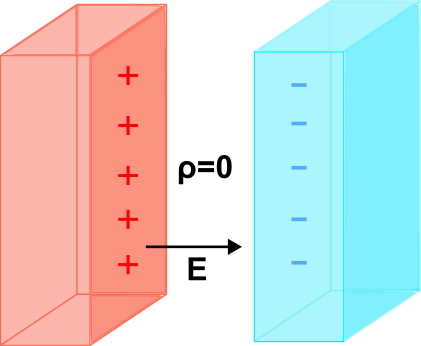
\includegraphics[width=0.38\textwidth]{images/lap} % sostituisci con il nome dell'immagine
    \vspace{0.5cm}
\end{wrapfigure}

Consideriamo un sottocaso dell'equazione di Poisson valide nelle regioni in cui non \`e presente una distribuzione di carica $\rho = 0$. L'equazione di Poisson (1.30) assume la forma 
\begin{equation}
	\nabla^2\phi = 0
\end{equation}

che prende il nome di \textit{equazione di Laplace}.
Questa eqauzione ha soluzione banale per $\phi = 0$, ma soluzioni non banali se si devono soddisfare delle condizioni al contorno; come per esempio in figura. 
\\
Il problema generale dell'elettrostatica consiste proprio nel trovare il potenziale elettrico a partire da una distribuzione $ \rho$, e la sua risoluzione pu\`o essere molte volte ricondotto al cercare una soluzione per l'equazione di Laplace.  

\newpage


\section{Coordinate curvilinee ortogonali}

Fino a questo punto si sono utilizzate le coordiante cartesiane per descrivere gli operatori geadiente, rotazione e divergenza, in questa sezione definiamo degli strumenti matematici che ci permettono di generalizzare questi oggetti per diversi sistemi di coordinate. 
\\

In generale, possiamo descrivere un punto $\bold{x} \in \mathbb{R}^3$ usando le coordinate u,v,w in modo tale che $\bold{x} = \bold{x}(u,v,w)$. Se immaginiamo una variazione infinitesima questa viene descritta dal differenziale del punto
\begin{equation*}
	d\bold{x} = \frac{\partial \bold{x}}{\partial u} du \;+\; \frac{\partial \bold{x}}{\partial v}dv \; + \; \frac{\partial \bold{x}}{\partial w}dw
\end{equation*}
dove ciascuna componente definisce un vettore per le linee di superficie fissate le altre due variabili. Le coordinate (u,v,w) vengono definite \textit{ortogonali e curvilinee} se i vettori tangenti rispettivi sono ortogonali tra loro.
\\

Per delle coordinate curvilinee possiamo sempre definire vettori ortonormali tangenti alle rispettive linee di superficie normalizzandoli. 
\begin{equation*}
	\frac{\partial \bold{x}}{\partial u}=h_u \bold{e}_u \quad,\quad \frac{\partial \bold{x}}{\partial v} = h_v \bold{e}_v \quad , \quad \frac{\partial \bold{x}}{\partial w} = h_w \bold{e}_w
\end{equation*}
dove si sono introdotti i fattori di scala $h_u,h_v,h_w >0$ e i versori $\bold{e}_{v},\bold{e}_{v}$ e $\bold{e}_w$ formano un base ortonormale per cui $\bold{e}_{u} \times \bold{e}_{v} = \bold{e}_{w}$. Possiamo riscrivere il differenziale tenendo conto dei fattori di scala, e dunque
\begin{equation}
	d \mathbf{x}=h_u \mathbf{e}_u d u+h_v \mathbf{e}_v d v+h_w \mathbf{e}_w d w
\end{equation}

\subsubsection{Coordinate cartesiane}
Per le coordinate cartesiane un punto $\bold{x} \in \mathbb{R}^3$ \`e descritto rispetto alle coordinate ortonormali (x,y,z). Se prendiamo il differenziale del punto avremo che l'equazione (1.33) diventa
\begin{equation*}
	d\bold{x} = \text{dx} \; \bold{e}_{x} + \text{dy} \; \bold{e}_{y} + \text{dz} \; \bold{e}_{z}
\end{equation*}
e dunque i fattori di scala sono pari a $h_z = h_y = h_z =1$.

\subsubsection{Coordinate Cilindriche}
Un punto $\bold{x} \in \mathbb{R}^3$ nello spazio \`e descritto dalle coordinate cilindriche rispetto alle variabili $(R\cos\theta,R \sin \theta, z)$ dove $R > 0$ e $\theta \in [0,2\pi]$. L'inversa della trasformazione di coordinate \`e data da 
\begin{equation*}
	R = \sqrt {x^2+y^2} \quad \text{e} \quad \tan \theta = \frac{y}{x}
\end{equation*}

applicando la matrice Jacobiana associata agli elementi della base $\{\bold{e}_1,\bold{e}_2,\bold{e}_3\}$ determiniano la base $\{\bold{e}_{r},\bold{e}_{\theta},\bold{e}_{z}\}$ rispetto al nuovo sistema di coordinate cilindriche 
\begin{equation*}
	\mathcal{J} = \left [ \begin{array}{ccc}
		\cos\theta & -R \sin \theta & 0 \\
		\sin \theta & R \cos \theta & 0 \\
		0 & 0 & 1 
	\end{array} \right ]
\end{equation*}
e dunque 
\begin{equation*}
	\begin{aligned}
& \mathbf{e}_R=\hat{\boldsymbol{R}}=(\cos \theta, \sin \theta, 0) \\
& \mathbf{e}_\theta=\hat{\boldsymbol{\theta}}=(-\sin \theta, \cos \theta, 0) \\
& \mathbf{e}_z=\hat{\mathbf{z}}
\end{aligned}
\end{equation*}
dove 
\begin{equation*}
	h_R = h_z =1 \quad \text{e} \quad h_{\theta} = R
\end{equation*}

\subsubsection{Coordinate Polari}
Per un punto nello spazio definiamo le coordinate sferiche come
\begin{equation*}
	\mathbf{x}=(r \sin \theta \cos \phi, r \sin \theta \sin \phi, r \cos \theta)
\end{equation*}
con $r \geq 0$, $\theta \in [0,\pi]$ e $\phi \in [0,2\pi)$. L'inversa \`e data da
\begin{equation*}
	r=\sqrt{x^2+y^2+z^2} \quad, \quad \tan \theta=\frac{\sqrt{x^2+y^2}}{z} \quad, \quad \tan \phi=\frac{y}{x}
\end{equation*}
Ripetendo quanto fatto per le coordinate cilindriche, la base rispetto alle coordinate sferiche \`e data da
\begin{equation*}
	\begin{aligned}
& \mathbf{e}_r=\hat{\mathbf{r}}=(\sin \theta \cos \phi, \sin \theta \sin \phi, \cos \theta) \\
& \mathbf{e}_\theta=\hat{\boldsymbol{\theta}}=(\cos \theta \cos \phi, \cos \theta \sin \phi,-\sin \theta)\\ 
\end{aligned}
\end{equation*}

\begin{equation*}
 \mathbf{e}_\phi=\hat{\boldsymbol{\phi}}=(-\sin \phi, \cos \phi, 0)	
\end{equation*}
I fattori di scala sono invece dati da
\begin{equation*}
	h_r=1 \quad, \quad h_\theta=r \quad, \quad h_\phi=r \sin \theta
\end{equation*}
Ora che abbiamo definito come cambiano in fattori di scala per diversi sistemi di coordinate, determiniamo la rappresentazione degli operatori visti nelle sezioni precedenti.

\subsection{Gradiente}

L'operatore gradiente \`e uno dei pi\`u semplici da determinare in quanto il differenziale si lega al gradiente di un campo scalare mediante nel seguente modo
\begin{equation*}
	df = \nabla f \cdot d\bold{x}
\end{equation*}
Per un sistema di coordinate generico questa espressione assume la forma esplicita
\begin{equation*}
	d f=\frac{\partial f}{\partial u} d u+\frac{\partial f}{\partial v} d v+\frac{\partial f}{\partial w} d w=\nabla f \cdot\left(h_u \mathbf{e}_u d u+h_v \mathbf{e}_v d v+h_w \mathbf{e}_w d w\right)
\end{equation*}
Usando l'ortonormalit\`a degli elementi della base vettoriale, e comparando i termini di destra con quelli di sinistra possiamo riscrivere il gradiente come 
\begin{equation}
	\nabla f=\frac{1}{h_u} \frac{\partial f}{\partial u} \mathbf{e}_u+\frac{1}{h_v} \frac{\partial f}{\partial v} \mathbf{e}_v+\frac{1}{h_w} \frac{\partial f}{\partial w} \mathbf{e}_w
\end{equation}
Utilizzando i fattori di scala determinati precedentemente abbiamo che il gradiente in coordinate cilindriche per una funzione $f(r,\theta,z)$ \`e 
\begin{equation*}
	\nabla f=\frac{\partial f}{\partial r} \hat{\boldsymbol{r}}+\frac{1}{r} \frac{\partial f}{\partial \theta} \hat{\boldsymbol{\theta}}+\frac{\partial f}{\partial z} \hat{\mathbf{z}}
\end{equation*}
In coordinate polari, il gradiente di una funzione $f(r,\theta,\phi)$ \`e 
\begin{equation*}
	\nabla f=\frac{\partial f}{\partial r} \hat{\mathbf{r}}+\frac{1}{r} \frac{\partial f}{\partial \theta} \hat{\boldsymbol{\theta}}+\frac{1}{r \sin \theta} \frac{\partial f}{\partial \phi} \hat{\boldsymbol{\phi}}
\end{equation*}
\newpage

\subsection{Rotore e Divergenza}

Per costruire gli operatori differenziali di divergenza e rotazione rispetto a delle coordinate generalizzate, definiamo prima l'operatore nabla per delle coordinate generiche 
\begin{equation}
	\nabla=\frac{1}{h_u} \mathbf{e}_u \frac{\partial}{\partial u}+\frac{1}{h_v} \mathbf{e}_v \frac{\partial}{\partial v}+\frac{1}{h_w} \mathbf{e}_w \frac{\partial}{\partial w}
\end{equation}
Dato un campo vettoriale $\bold{F}(u,v,w)$ definito rispetto a delle generiche coordinate ortogonali e curvilinee, la divergenza \`e data da
\begin{equation}
	\nabla \cdot \mathbf{F}=\frac{1}{h_u h_v h_w}\left(\frac{\partial}{\partial u}\left(h_v h_w F_u\right)+\frac{\partial}{\partial v}\left(h_u h_w F_v\right)+\frac{\partial}{\partial w}\left(h_u h_v F_w\right)\right)
\end{equation}
e la rotazione \`e data dal determinante 
\begin{equation}
	\nabla \times \mathbf{F}=\frac{1}{h_u h_v h_w}\left|\begin{array}{ccc}
h_u \mathbf{e}_u & h_v \mathbf{e}_v & h_w \mathbf{e}_w \\
\frac{\partial}{\partial u} & \frac{\partial}{\partial v} & \frac{\partial}{\partial w} \\
h_u F_u & h_v F_v & h_w F_w
\end{array}\right|
\end{equation}
In coordinate cilindriche abbiamo che divergenza e rotore assumono l'espressione
\begin{equation*}
	\begin{aligned}
		&\nabla \cdot \mathbf{F}=\frac{1}{\rho} \frac{\partial\left(\rho F_\rho\right)}{\partial \rho}+\frac{1}{\rho} \frac{\partial F_\phi}{\partial \phi}+\frac{\partial F_z}{\partial z} \\[0.5cm]
		& \nabla \times \mathbf{F}=\left(\frac{1}{\rho} \frac{\partial F_z}{\partial \phi}-\frac{\partial F_\phi}{\partial z}\right) \hat{\boldsymbol{\rho}}+\left(\frac{\partial F_\rho}{\partial z}-\frac{\partial F_z}{\partial \rho}\right) \hat{\boldsymbol{\phi}}+\frac{1}{\rho}\left(\frac{\partial\left(\rho F_\phi\right)}{\partial \rho}-\frac{\partial F_\rho}{\partial \phi}\right) \hat{\mathbf{z}}&
	\end{aligned}
\end{equation*}
mentre per le coordinate sferiche 
\begin{equation*}
	\begin{aligned}
		&\nabla \cdot \mathbf{F}=\frac{1}{r^2} \frac{\partial\left(r^2 F_r\right)}{\partial r}+\frac{1}{r \sin \theta} \frac{\partial\left(\sin \theta F_\theta\right)}{\partial \theta}+\frac{1}{r \sin \theta} \frac{\partial F_\phi}{\partial \phi}\\[0.5cm]
		&\begin{aligned}
\nabla \times \mathbf{F}= & \frac{1}{r \sin \theta}\left(\frac{\partial\left(\sin \theta F_\phi\right)}{\partial \theta}-\frac{\partial F_\theta}{\partial \phi}\right) \hat{\mathbf{r}} +\frac{1}{r}\left(\frac{1}{\sin \theta} \frac{\partial F_r}{\partial \phi}-\frac{\partial\left(r F_\phi\right)}{\partial r}\right) \hat{\boldsymbol{\theta}} 
+\frac{1}{r}\left(\frac{\partial\left(r F_\theta\right)}{\partial r}-\frac{\partial F_r}{\partial \theta}\right) \hat{\boldsymbol{\phi}}
\end{aligned}
	\end{aligned}
\end{equation*}
I risultati (1.35) e (1.36) sono dovuti al fatto che il campo vettoriale deve essere espresso rispetto alla base generalizzata e dunque deve tenere conto dei fattori di scala.
\newpage

\subsection{Laplaciano}

Utilizzando l'espressione (1.34) e (1.36), possiamo esprimere il Laplaciano di un campo scalare per un generico sistema di coordinate come
\begin{equation}
	\nabla^2 f=\nabla \cdot \nabla f=\frac{1}{h_u h_v h_w}\left[\frac{\partial}{\partial u}\left(\frac{h_v h_w}{h_u} \frac{\partial f}{\partial u}\right)+\frac{\partial}{\partial v}\left(\frac{h_u h_w}{h_v} \frac{\partial f}{\partial v}\right)+\frac{\partial}{\partial w}\left(\frac{h_u h_v}{h_w} \frac{\partial f}{\partial w}\right)\right]
\end{equation}
In coordinate cilindriche avremo
\begin{equation*}
	\nabla^2 f=\frac{1}{\rho} \frac{\partial}{\partial \rho}\left(\rho \frac{\partial f}{\partial \rho}\right)+\frac{1}{\rho^2} \frac{\partial^2 f}{\partial \phi^2}+\frac{\partial^2 f}{\partial z^2}
\end{equation*}
mentre in coordinate polari assume la forma 
\begin{equation*}
	\nabla^2 f=\frac{1}{r^2} \frac{\partial}{\partial r}\left(r^2 \frac{\partial f}{\partial r}\right)+\frac{1}{r^2 \sin \theta} \frac{\partial}{\partial \theta}\left(\sin \theta \frac{\partial f}{\partial \theta}\right)+\frac{1}{r^2 \sin ^2 \theta} \frac{\partial^2 f}{\partial \phi^2}
\end{equation*}

\subsection{Esempi ed Esercizi}

\subsubsection{Distribuzioni di carica a simmetria cilindrica}

\begin{wrapfigure}{r}{0.5\textwidth}
  \centering
  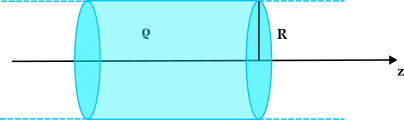
\includegraphics[width=0.5\textwidth]{images/cilindro}
\end{wrapfigure}

Consideriamo una distribuzione di carica $\rho$ per un cilindro di raggio R e lunghezza infinita. Vogliamo calcolarne il campo utilizzando la prima legge di Maxwell.

Per ragioni di simmetria si ha che il campo ha direzione radiale $\bold{E} = E_r(r)\hat{\mu}_r$ e dunque la forma differenziale della legge di Gauss assume la forma 
\begin{equation*}
	\frac{1}{r} \frac{\partial (r E_r)}{\partial r} = \frac{\rho}{\varepsilon_0}
\end{equation*}
risolvendo per quadrature si ha che 
\begin{equation*}
	\bold{E} = \frac{\rho r}{2 \varepsilon_0}\hat{\mu}_{r} +\frac{B}{r}\hat{\mu}_r
\end{equation*}
Per determinare il valore della costante d'integrazione B, possiamo osservare che se misuriamo la forza su una carica $q_0$ nel centro della distribuzione per $r = 0$ si ha che per ragioni di simmetria la forza esercitata \`e $\bold{F} = 0$. Dunque $B=0$.
\\

Dato che all'esterno della distribuzione non \`e presente carica, si ha che 
\begin{equation*}
		\frac{1}{r} \frac{\partial (r E_r)}{\partial r} = 0
\end{equation*}
e dunque 
\begin{equation*}
	\bold{E}_{ext} = \frac{B}{r}
\end{equation*}
utilizzando le condizioni al contorno per la regione cilindrica si ha che 
\begin{equation*}
	\bold{E}_{ext}(r=R) = \bold{E}_{int}(r=R) \iff \frac{\rho R}{2 \varepsilon_0} = \frac{B}{R}
\end{equation*}
e quindi possiamo concludere che 
\begin{equation*}
B = \frac{\rho R^2}{2\varepsilon_0}
\end{equation*}
Il campo complessivamente \`e dato da 
\begin{equation*}
	E(r)= \left \{ \begin{array}{l}
		\frac{\rho r}{2 \varepsilon_0} \quad r \leq R \\
		\frac{\rho R^2}{2 \varepsilon_0} \frac{1}{r} \quad r \geq R
	\end{array} \right.
\end{equation*}
possiamo osservare che il campo esternamente alla distribuzione di carica\`e equivalente a 
\begin{equation*}
	E = \frac{\lambda}{2\pi \varepsilon_0} \frac{1}{r}
\end{equation*}
che \`e quello di un filo infinito con densit\`a di carica lineare $\lambda$.

\subsubsection{Equazione di Poisson per una carica puntiforme}

Consideriamo una densit\`a di carica come una distribuzione
\begin{equation*}
	\rho(\bold{r}) = \delta(\bold{r}) = \left \{ \begin{array}{l}
		0 \quad  \bold{r} > 0 \\
		\neq 0 \quad \bold{r} = 0
	\end{array}\right.
\end{equation*}
dove vale la relazione $\int_{V}\rho dV = q$, per ogni volume che contiene l'origine in cui \`e posta al carica puntiforme q.
Verifichiamo l'equazione di Poisson in due modi:
\begin{enumerate}
	\item In modo esplicito risolvendo l'equazione differenziale $\nabla^2\phi = 0$ per $\bold{r} > 0$
	\item In forma integrale per $\bold{r} \to 0$ usando il teorema della divergenza 
	\begin{equation*}
		\int_{V} \nabla^2\phi dV = -\frac{1}{\varepsilon_0}\int_{V} \delta(\bold{r})dV = -\frac{q}{\varepsilon_0}
	\end{equation*}
\end{enumerate}
1) Siccome il problema \`e a simmetria sferica, consideriamo il Laplaciano in coordinate sferiche e dunque otteniamo l'equazione differenziale
\begin{equation*}
	\nabla^2\phi = \frac{1}{r^2}\frac{\partial }{\partial r} \left (r^2 \frac{\partial \phi}{\partial r} \right) = \frac{q}{4 \pi \varepsilon_0} \frac{1}{r^2} \frac{\partial }{\partial r} \left ( r^2 \frac{\partial}{\partial r} \left ( \frac{1}{r}\right)\right )= 0
\end{equation*}
\\
2)\begin{equation*}
	\int_{V} \nabla^2\phi dV = \int_{V}\nabla \cdot (\nabla \phi) dV = \int_{S}\nabla \phi \cdot d\bold{A}
\end{equation*}
dato che $\nabla^2\phi - 0$ per $\bold{r} \neq 0$, l'unico punto per cui l'integrale \`e non nullo \`e $\bold{r} = 0$. Presa una superficie qualsiasi che racchiude la carica nell'origine abbiamo che
\begin{equation*}
	\int_{S} \nabla \phi \cdot d \bold{A} =  \frac{q}{4 \pi \varepsilon_0}\int_{S} \frac{\partial}{\partial r} \left (\frac{1}{r} \right)\hat{\mu}_{r} \cdot d\bold{A} = - \frac{q}{4 \pi \varepsilon_0} \frac{1}{r^2} (4 \pi r^2)= - \frac{q}{\varepsilon_0} = - \frac{1}{\varepsilon_0}\int_{V} \delta(\bold{r}) dV
\end{equation*} 
e dunque possiamo concludere che 
\begin{equation*}
	\nabla^2\phi = - \frac{\rho}{\varepsilon_0}
\end{equation*}
Dato che abbiamo dimostrato che $\phi = \frac{q}{4 \pi \varepsilon_0} \frac{1}{r}$ \`e la soluzione dell'equazione di Poisson per una carica puntiforme e l'equazione di Poisson \`e lineare, possiamo concludere che la soluzione generale segue dal principio di sovrapposizione.


\section{Conduttori e Isolanti}


Un conduttore \`e una regione di spazio che contiene cariche che sono libere di muoversi. Per esempio i metalli sono tendenzialmente dei buoni conduttori. Come interagiscono questi materiali in presenza di cariche statiche ? a riguardo possiamo trarre le seguenti conclusioni
\begin{itemize}
	\item All'interno di un conduttore il campo elettrostatico $\bold{E} = 0$ \`e nullo
	\item Dato che $\bold{E}  = 0$ all'interno di un conduttore, il potenziale elettrostatico $\phi$ deve essere costante attraverso di esso.
	\item Siccome $\bold{E} = 0$ e vale la prima legge di Maxxwell $\nabla \cdot \bold{E} = \rho  \slash  \varepsilon_0$, si deve vere che $\rho = 0$. Di conseguenza all'interno del conduttore non pu\`o essere presente nessuna carica.
	\item I conduttori possono avere carica neutra, ovvero possiedono carica positiva e negativa che si bilanciano tra loro. Se un conduttore non \`e neutro, e quindi ha un eccesso di carica in uno dei due segni, questa \`e distribuita sulla sua superficie.
	\item Poich\`e $\phi$ \`e costante internamente al conduttore si ha che la superficie che lo racchiude \`e equipotenziale e dunque il campo elettrostatico $\bold{E} = - \nabla \phi$ \`e perpendicolare ad essa.
	\item Se \`e presente della carica di superficie $\sigma $ in qualsiasi parte del conduttore, la discussione della discontinuit\`a del campo insieme al fatto che $\bold{E} = 0$ all'interno, ci dice che il campo elettrico all'esterno del conduttore \`e 
	\begin{equation*}
		\bold{E} = \frac{\sigma}{\varepsilon_0} \hat{\bold{n}}
	\end{equation*}
\end{itemize}

I problemi che interessano i conduttori hanno una natura diversa da quelli affrontati fin'ora. Il motivo \`e che non conosciamo la distribuzione di carica del conduttore in partenza, dunque non possiamo utilizzare gli strumenti precedentemente definiti. Quello che osserviamo sperimentalmente \`e frutto di un interazione con una sorgente di campo $\bold{E}$ esterna che fa s\`i che le cariche interne al conduttore si riorganizzino in modo tale che il campo elettrico interno si annulli con quello esterno 
\begin{equation*}
	\bold{E}_{int} = \bold{E}_{ext} + \bold{E^*}_{int} = 0
\end{equation*}
In generale questo vuol dire che anche conduttori neutri finisco con una distribuzione di carica di superficie, negativa in alcuni punti e positiva in altri, in modo tale che il campo totale interno sia $\bold{E} = 0$.
\newpage
\begin{minipage}{0.5\textwidth}
    \centering
    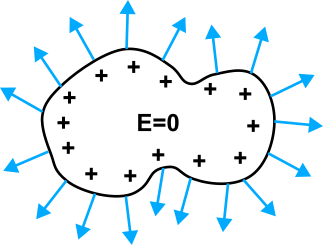
\includegraphics[width=0.8\textwidth]{images/isolanti.png}
    \captionof{figure}{Conduttore carico isolante}
\end{minipage}%
\begin{minipage}{0.5\textwidth}
    \centering
    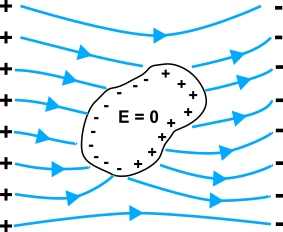
\includegraphics[width=0.8\textwidth]{images/conduct}
    \captionof{figure}{Conduttore neutro }
\end{minipage}
\\

Esistono anche dei materiali che prendono il nome di \textit{isolanti}, questi si elettrizzano facilmente e mantengono indefinitamente il proprio stato di carica. La distinzione tra conduttore ed isolante dipende dal contesto, ovvero dalla scala di tempo del fenomeno rispetto alla scala di tempo del movimento delle cariche. I fattori di risposta dipendono tipicamente dalla temperatura.

\subsubsection{Energia potenziale di una sfera carica di raggio R}

Per una sfera piena si ha che l'energia potenziale configurazionale \`e data da 
\begin{equation*}
	U_c = \frac{Q}{8 \pi \varepsilon_0} \frac{1}{R}
\end{equation*}
mentre per una sfera piena
\begin{equation*}
	U_p = \frac{6}{5} \frac{Q^2}{8 \pi \varepsilon_0} \frac{1}{R}
	\end{equation*}
Dunque in un conduttore a simmetria sferica, la ridistribuzione delle cariche in eccesso sulla superficie  esterna \`e una configurazione energeticamente favorevole, dato che $U_p > U_c$.
In  una sfera la carica di distribuisce in modo uniforme sulla superficie esterna  ( si pu\`o dimostrare che rappresenta la configurazione di minima energia potenziale).
\\
Se il conduttore non \`e sferico la carica si addensa nelle regioni con raggio di curvatura minore, si ha un "effetto punta".
\newpage
\subsubsection{Esempio - Effetto Punta}

Prendiamo un sistema formato da due sfere conduttrici di raggio $R_1 < R_2$ e collegate da un filo. Come si distribuisce la carica sulle rispettive superfici ?
\begin{figure}[!ht]
\vspace{0.2in}
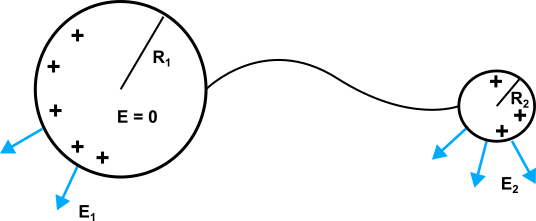
\includegraphics[width = 10cm]{images/punta}	
\centering
\vspace{0.2in}
\end{figure} 

La carica complessiva del sistema \`e data da $Q = Q_1 + Q_2$ dato che le due sfere sono collegate tra loro da un filo e quindi possiamo assumerlo come un sistema unico. Essendo sfere conduttrici internamente il campo $\bold{E} = 0$. Esternamente abbiamo quello di una carica puntiforme e di conseguenza il potenziale \`e dato da
\begin{equation*}
	\phi_1 = \frac{\sigma_1 R_1}{\varepsilon_0} \quad \text{e} \quad \sigma_2 = \frac{\sigma_2 R_2}{\varepsilon_0}
\end{equation*}
Dato che le due sfere conduttrici sono collegate tra loro si trovano allo stesso potenziale e dunque 
\begin{equation}
	\sigma_1R_1 =\sigma_2R_2
\end{equation}
Il risultato (1.39) ci dice che la densit\`a superficiale \`e proporzionale al reciproco del raggio di curvatura, di conseguenza avremo che la carica si addensa maggiormente sulla superficie della sfera con raggio  minore. Possiamo estendere tale risultato a superfici generiche e quindi concludere che, la carica ha densit\`a maggiore laddove il raggio di curvatura \`e il minore possibile.

\subsection{Induzione Totale}

 Consideriamo un sistema isolato in cui \`e presente una sfera conduttrice, in cui \`e presente una cavit\`a contente una carica puntiforme q. Dato che all'interno del conduttore $\bold{E}_{int} = 0$ se consideriamo una superficie Gaussiana che racchiude la cavit\`a per la legge di Gauss si ha che 
 \begin{wrapfigure}{r}{0.5\textwidth}  % 'r' for right, 0.5\textwidth for image width
    \centering
    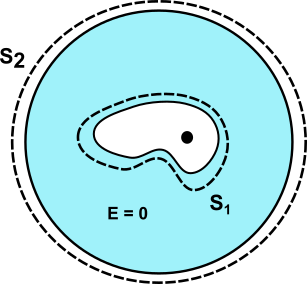
\includegraphics[width=0.46\textwidth]{images/inductor}  % Adjust image width as necessary
\end{wrapfigure}
 \begin{equation*}
 	\frac{1}{\varepsilon_0}\int_{V}dV \; \rho = \int_{S} \bold{E} \cdot d\bold{A} = 0
 \end{equation*}
 e quindi 
 \begin{equation*}
 	Q = q +Q_{int} = 0 \Rightarrow Q_{int} = -q
 \end{equation*}
 Dunque si induce una carica sulla superficie interna della cavit\`a di segno opposto rispetto alla sorgente al suo interno. Se prendiamo una superficie Gaussiana $S_2$ esterna che racchiude il conduttore avremo per la legge di Gauss che 
 \begin{equation*}
 	\int_{S_2}\bold{E} \cdot d\bold{A} = \frac{q}{\varepsilon_0}
 \end{equation*}
 e dunque sulla superficie esterna  avremo una carica
 \begin{equation*}
 	Q_{ext} = q = -Q_{int}
 \end{equation*}
 Per quanto discusso possiamo concludere che per un generico conduttore, la forma del campo elettrico esterno non dipende dalla posizione della carica sorgente posta al suo interno, ma dalla geometria del conduttore stesso. Complessivamente avremo che il campo, per il principio di sovrapposizione \`e dato dai contributi
 \begin{equation*}
 	\bold{E} = \bold{E}_q + \bold{E}_{ind}^{int} + \bold{E}_{ext}^{ind} = \bold{E}_{ext}^{ind}
 \end{equation*}
 dove 
 \begin{equation*}
 	\bold{E}_q + \bold{E}_{ind}^{int} = 0
 \end{equation*}
 dato che la carica sulla superficie esterna \`e distribuita uniformemente. Tale risultato \`e valido per qualsiasi raggio R. 
 Se il conduttore non \`e omogeneo  i risultati sulla carica indotta sono ancora validi solo che il campo esterno non sar\`a pi\`u a simmetria sferica perch\`e la distribuzione di carica non \`e pi\`u uniforme.
 
 \newpage
 
 \subsubsection{Esempio - Induzione con una carica esterna}
 
\begin{figure}[!ht]
\vspace{0.1in}
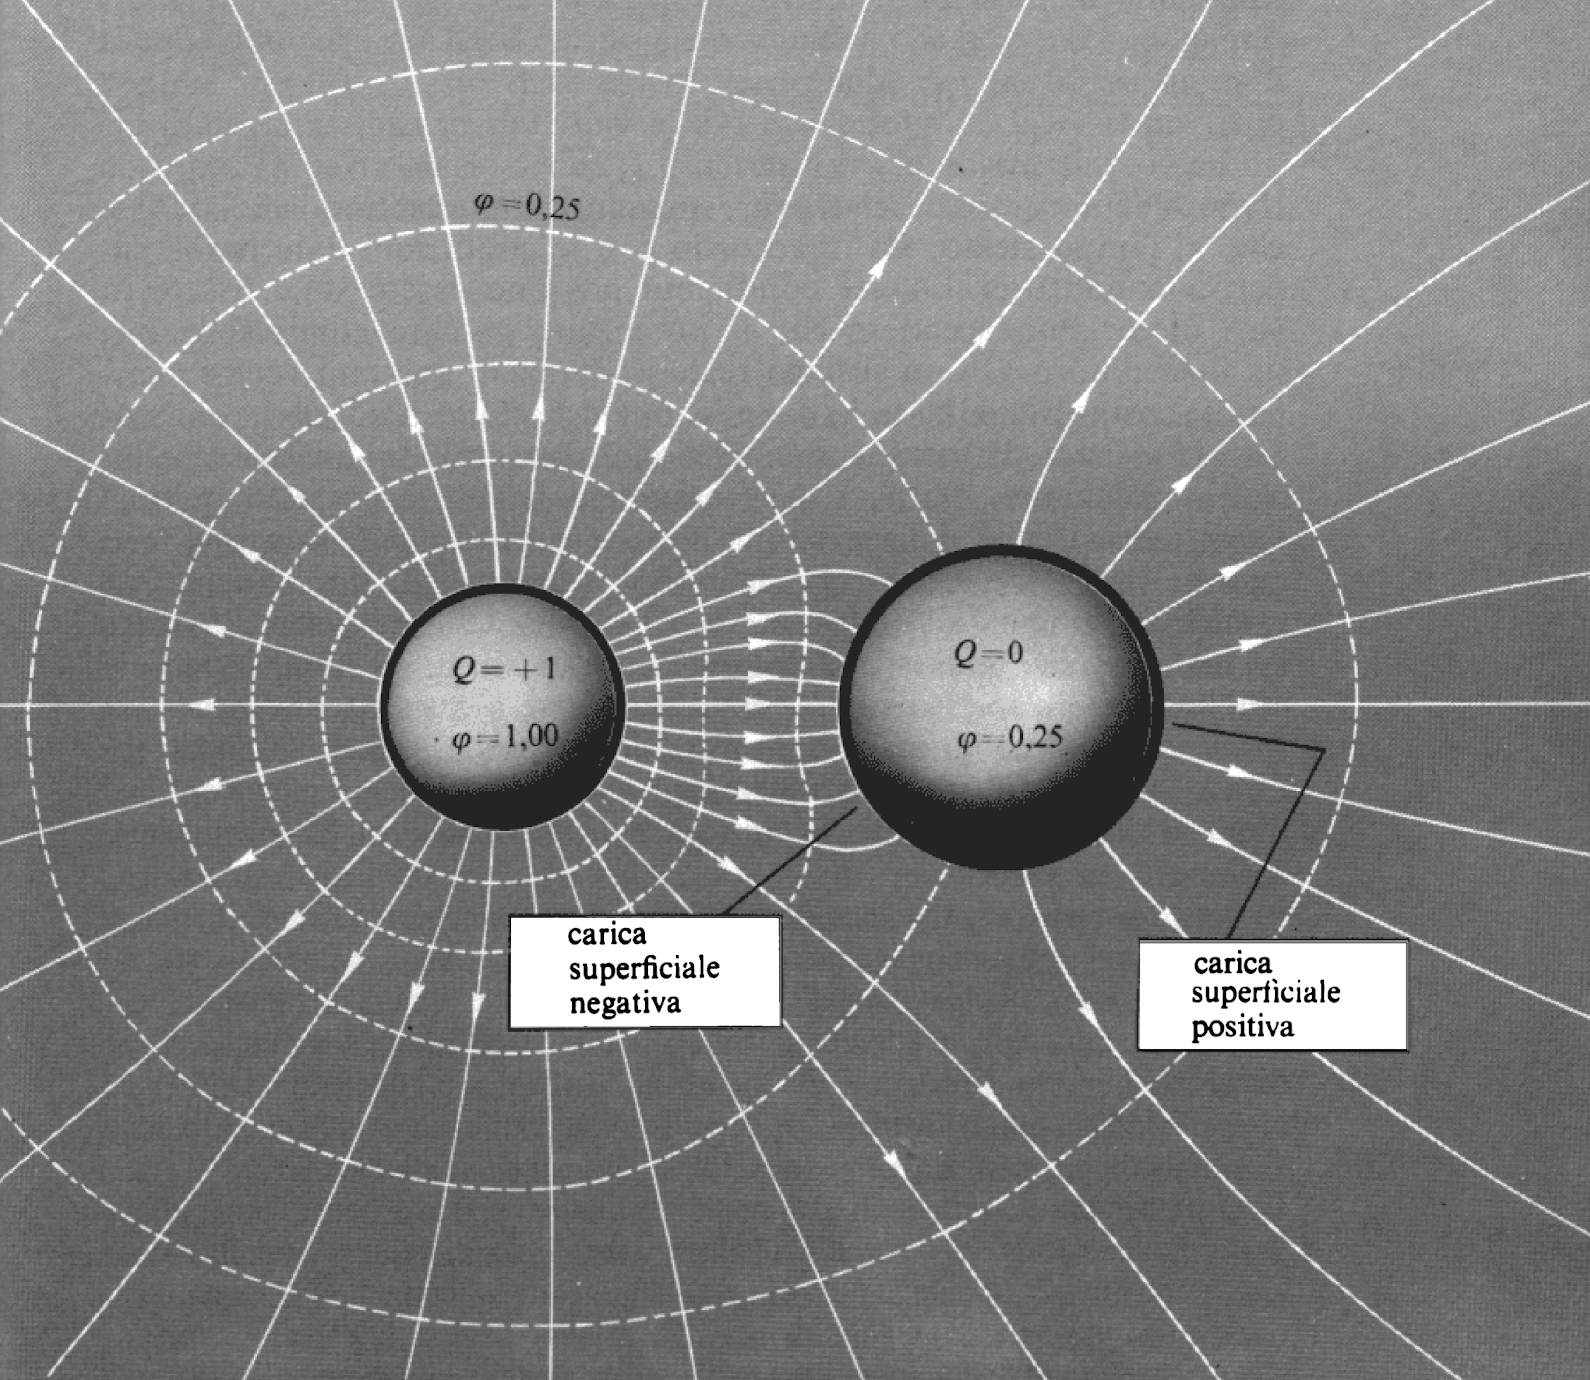
\includegraphics[scale = 0.35]{images/conductor}	
\centering
\vspace{0.1in}
\end{figure}

 Consideriamo una distribuzione di carica a simmetria sferica e un conduttore con la medesima simmetria.
 Avremo che  sul conduttore non possono esserci linee di campo che iniziamo e terminano sulla sua superficie. Per la sorgente di carica le linee di campo sono a simmetria radiale in lontananza. La carica indotta sul conduttore si divide in
 \begin{equation*}
 	Q_{ind} = \left \{ \begin{array}{l}
 		Q > 0 \quad \text{per la superficie interna}\\
 		Q< 0 \quad \text{per la superficie esterna }
 	\end{array}\right.
 \end{equation*}
 Non tutte le linee di campo si possono chiudere sul conduttore, alcune proseguono verso infinito di conseguenza la carica indotta sul conduttore in generale \`e minore di della carica della sorgente.
 \begin{equation*}
 	|Q_{ind}| < |Q|
 \end{equation*}
 Solo quando il conduttore racchiude la carica sorgente possiamo parlare d'induzione totale. 
 \newpage
 
 \subsection{Problema generale dell'elettrostatica: Il teorema di unicit\`a }
 
 Il problema dell'elettrostatica si riduce alla determinazione del campo elettrico a partire da una configurazione di cariche statiche. In linea di principio la soluzione dell'equazione di Maxwell 
 \begin{equation*}
 	\nabla \cdot \bold{E}  = -\frac{\rho}{\varepsilon_0}
 \end{equation*}
 \`e data da 
 \begin{equation*}
 	\bold{E} = \frac{1}{4 \pi \varepsilon_0} \int_{V} dV' \; \frac{\rho(\bold{r}')}{|\bold{r}-\bold{r}'|^2} \hat{u}_{rr'}
 \end{equation*}
 che possiamo ricondurre alla soluzione dell'equazione di Laplace dato che $ \phi = - \nabla \bold{E} $ e quindi
 \begin{equation*}
 	\phi(r) = \frac{1}{4 \pi \varepsilon_0} \int_{V} dV' \; \frac{\rho(\bold{r}')}{|\bold{r}-\bold{r}'|} 
 \end{equation*}
Tuttavia per i problemi che coinvolgono i conduttori la densit\`a di carica $\rho$ non \`e necessariamente nota a priori, per i seguenti motivi:
\begin{enumerate}
	\item La carica si ridistribuisce e in generale per un conduttore conosciamo solo la carica totale di un conduttore, ma non esattamente come \`e distribuita.
	\item Sperimentalmente siamo in grado di determinare solo il potenziale del conduttore.
\end{enumerate}
In questi casi \`e conveniente riformulare il problema , usando le relazioni espresse nelle equazioni di Laplace e Poisson in regioni in cui non \`e presenta della carica libera e rispetto a cui si possono formulare delle condizioni al contorno.

\subsubsection{Esempio}
\begin{wrapfigure}{r}{0.4\textwidth} % 'r' for right, 'l' for left
    \centering
    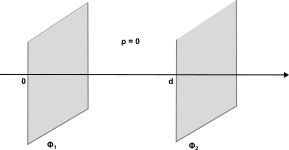
\includegraphics[width=0.4\textwidth]{images/laplacezero} % Replace with your image
\end{wrapfigure}
Prendiamo due piani conduttori infiniti posti in parallelo, nel volume compreso tra i due piani abbiamo carica nulla dunque l'equazione di Laplace \`e 
\begin{equation*}
	\nabla^2 \phi = 0
\end{equation*}
con condizioni al contorno $\phi(0) = \phi_1$ e $\phi(d) = \phi_2$, dove $\phi_2 > \phi_1$. Dato che il campo ha direzione solo lungo l'asse ortogonale ai piani, che consideriamo $x$, l'equazione di Laplace diventa
\begin{equation*}
	\frac{d^2\phi}{dx^2} = 0
\end{equation*}
che ha come soluzione 
\begin{equation*}
	\phi(x) = ax + b
\end{equation*}
Per determinare le costanti $a,b \in \mathbb{R}$, applichiamo le condizioni al contorno, 
\begin{equation*}
	\phi(0) = b = \phi_1 \quad ; \quad \phi(d) = ad+\phi_1 = \phi_2 \Rightarrow a = \frac{\phi_2 - \phi_1}{d}
\end{equation*}

\begin{wrapfigure}{r}{0.4\textwidth} % 'r' for right, 'l' for left
    \centering
    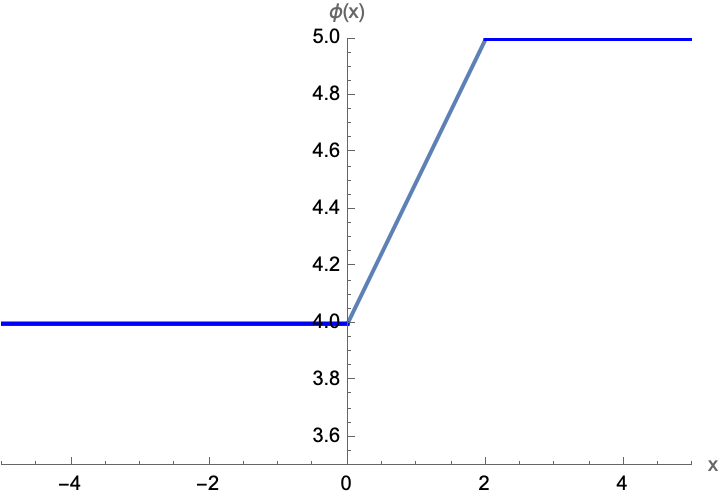
\includegraphics[width=0.4\textwidth]{images/planefield} % Replace with your image
\end{wrapfigure}

quindi il potenziale si comporta nel seguente modo
\begin{equation*}
	\phi(x) = \frac{\phi_2 -\phi_1}{d}x + \phi_1 \quad x \in [0,d]
\end{equation*}

Utilizzando il risultando per cui $\bold{E} = - \nabla  \phi $ abbiamo che il campo elettrico ha la seguente forma 
\begin{equation*}
	\bold{E} = -\frac{(\phi_2 -\phi_1)}{d}\hat{u}_x
\end{equation*}

\noindent I problemi risolti con la metodologia dell'esempio prendono il nome di \textit{problemi confinati}, sono una particolare categoria per cui \`e sempre possibile determinare una soluzione per integrazione. Questo \`e dovuto al fatto che si ha uno spazio chiuso , al cui interno sono presenti regioni di spazio connesse, che contengono della carica e permettono di definire delle condizioni al contorno per l'equazione di Laplace.
\begin{figure}[!ht]
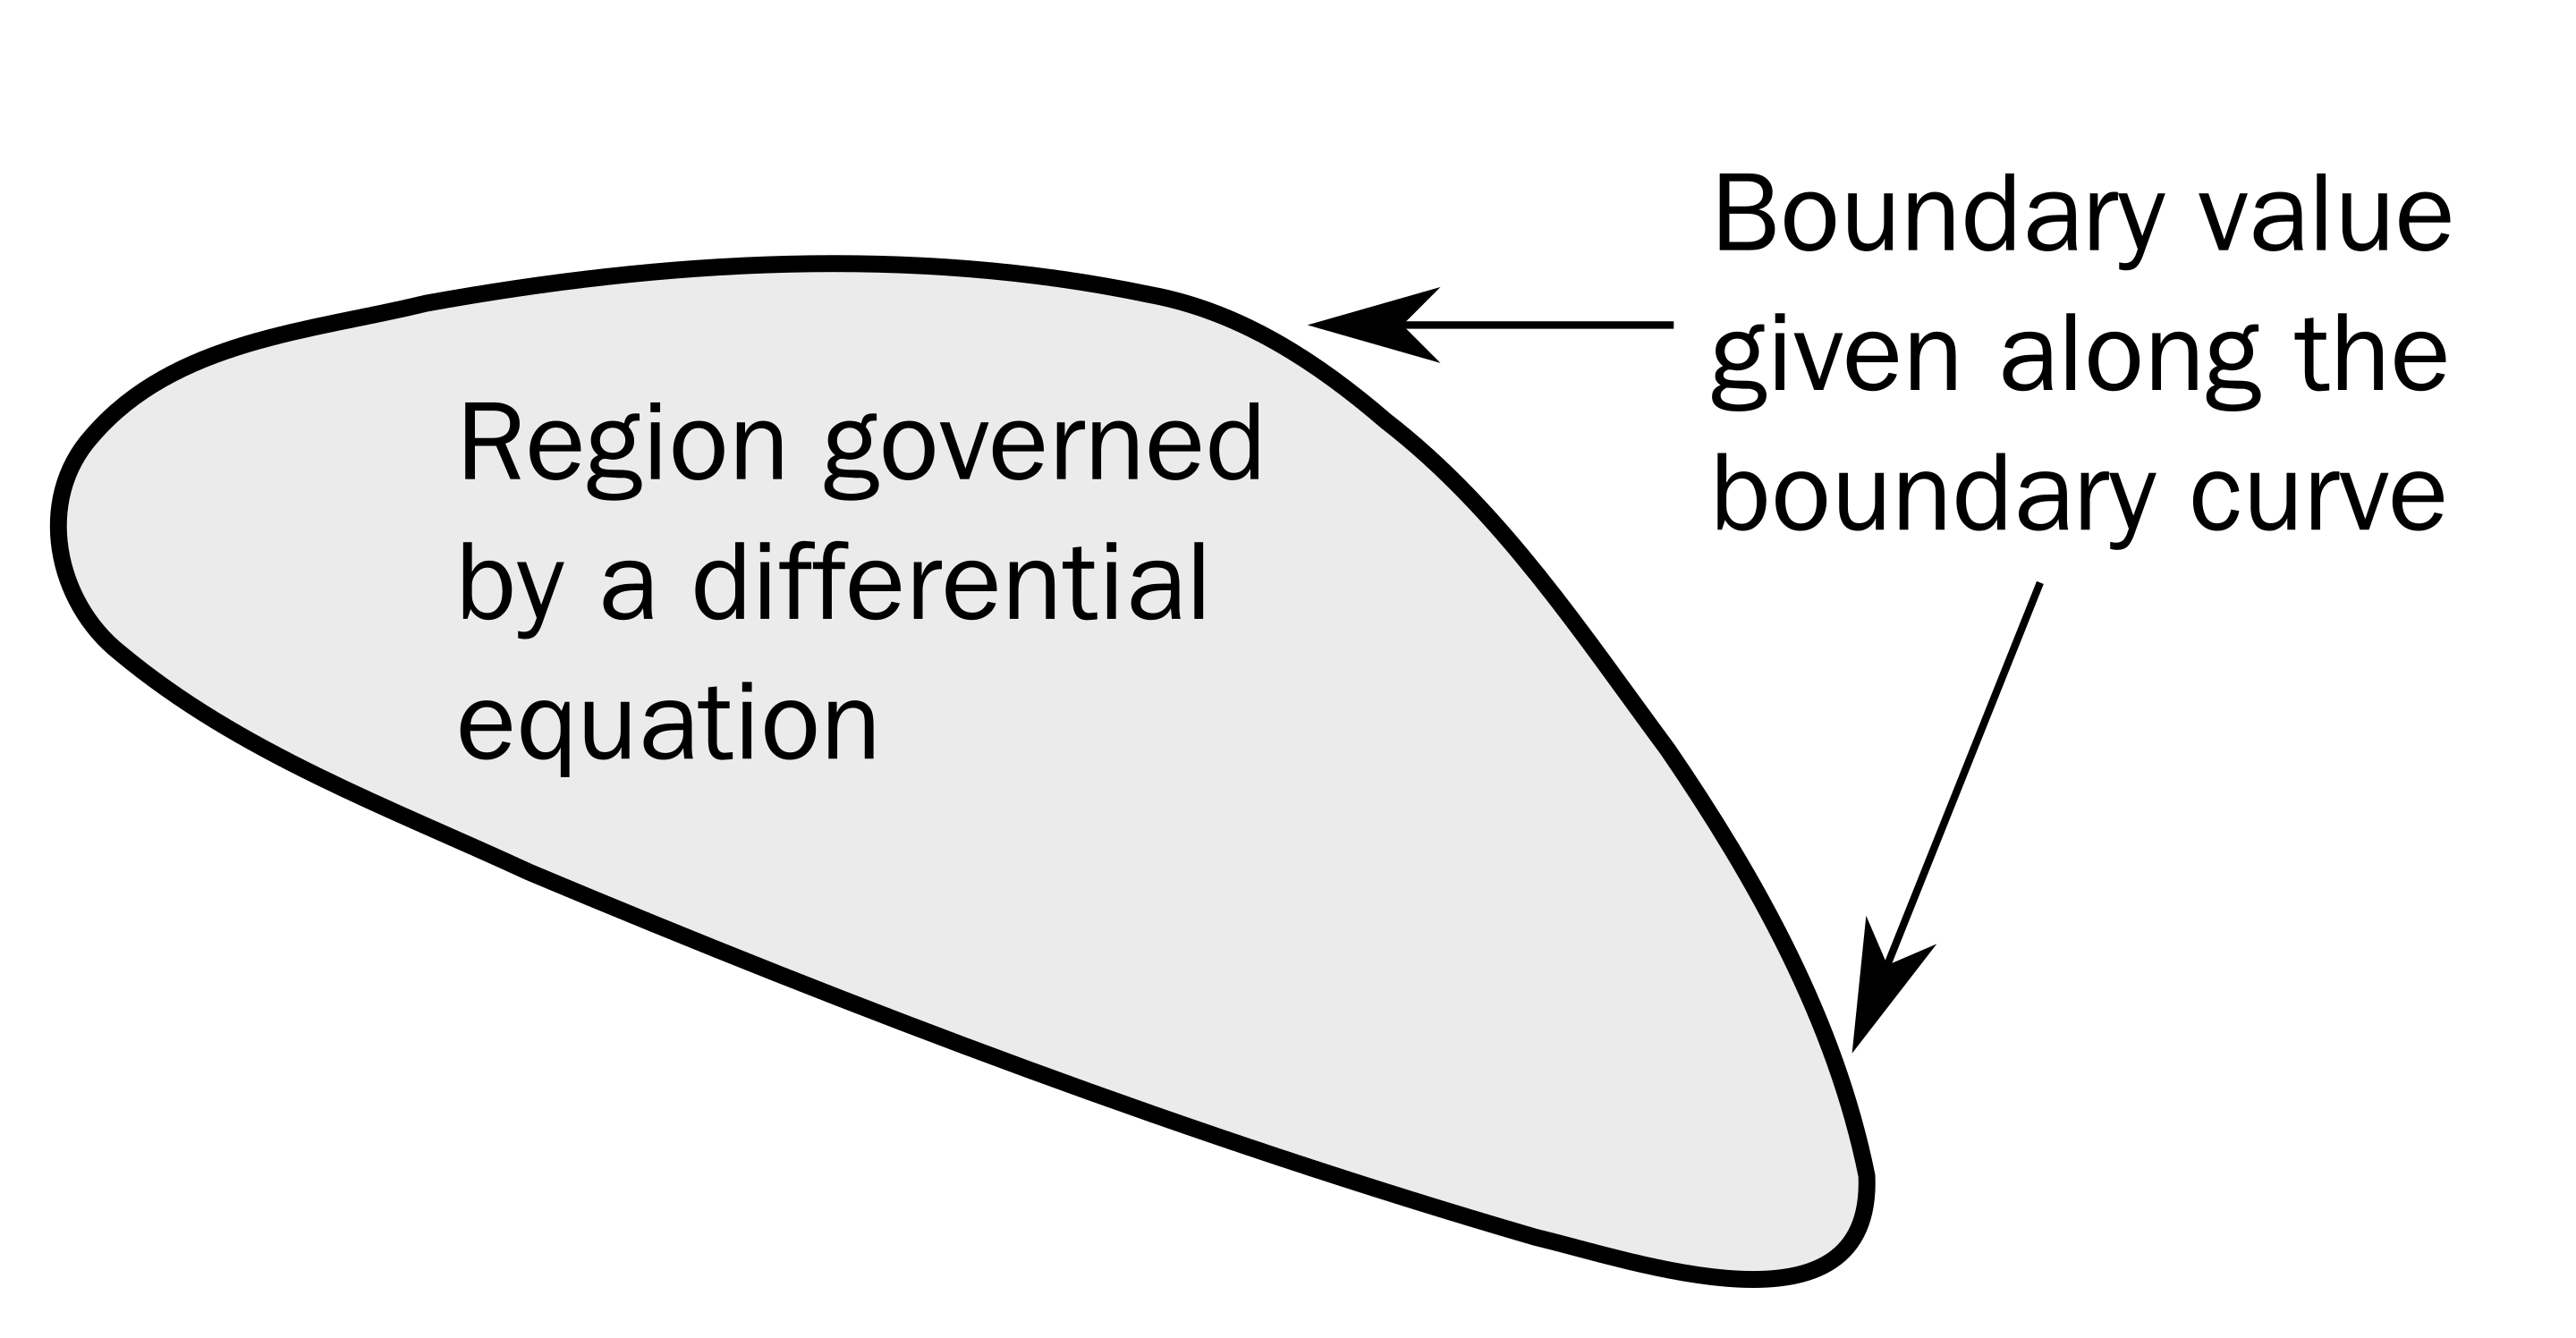
\includegraphics[width = 9cm]{images/boundaryproblem}
\centering
\end{figure}  

\noindent In generale questa tipologia di problemi pu\`o essere risolta utilizzando il metodo di separazione delle variabili.

In generale le soluzioni di questa categoria di problemi, deve soddisfare le seguenti proposizioni:

\begin{prop}
	Il potenziale elettrostatico in un generico punto C \`e uguale al valore medio del potenziale elettrostatico dato da una sfera che ha C come suo centro.
	\begin{equation*}
		\phi_C = \langle \phi_S \rangle 
	\end{equation*}
La seguente propriet\`a risulta essere verficata per tutte le funzioni per cui $\nabla \times \nabla\phi = 0$
\end{prop}
\begin{proof}
	Definiamo 
	\begin{equation*}
		\phi_C = \frac{q}{4\pi\varepsilon_0} \quad \text{e} \quad \langle \phi_S \rangle = \frac{1}{N} \sum_{i=1}^{N} \frac{q'}{4 \pi \varepsilon_0} \frac{1}{r_i} 
	\end{equation*}
Ipotizziamo di volere spostare una carica q ad una distanza r da una carica q' della sfera S, dovremo compiere un lavoro  $W = q \phi'(r) = q'\phi_C(r)$. Ora consideriamo il lavoro per spostare q ad una distanza r, dall'intera sfera, questo \`e dato da 
\begin{equation*}
	W = \frac{1}{N} \sum_{i} \frac{qq'}{4 \pi \varepsilon_0} \frac{1}{r_i} = q \langle \phi_S \rangle 
\end{equation*}
essendo il lavoro il medesimo avremo $\phi_C = \langle \phi_S \rangle $.

\end{proof}
\begin{prop}
	La funzione $\phi$ non possiede valori di estremo nella regione per cui \`e definita l'equazione $\nabla^2 \phi = 0$
\end{prop}
\begin{proof}
	Ipotizziamo per assurdo che esista un punto P nella regione in cui $\nabla^2 \phi = 0$, per cui $\phi(P) = \phi_{max}$ la funzione del potenziale assume valore massimo. Preso un intorno sferico attorno a P, avremo che per tutti i punti appartenenti alla sfera S vale $\phi_S < \phi(P)$, di conseguenza abbiamo un punto di equilibrio del sistema. Il che \`e assurdo perch\`e in una regione di spazio dove \`e definita l'equazione di Laplace non possono esserci configurazioni di equilibrio. (Non \`e vero in generale)
	 
\end{proof}
\begin{prop}
	La  soluzione dell'equazione di Laplace e Poisson \`e unica
\end{prop}
\begin{proof}
	Ipotizziamo che esistano due soluzioni $\phi_1$ e $\phi_2$ dell'equazione $\nabla^2 \phi = 0$ e che siano date le seguenti condizioni al contorno $\phi(\bold{x}_1) = \phi_1,..., \phi(\bold{x}_N) = \phi_N$. Definiamo la funzione $W(x) = \phi_2 - \phi_1$ e di conseguenza le condizioni al contorno diventano $W(\bold{x}_i) = 0$ per $i = 1,..,N$. La funzione W(x) \`e soluzione dell'equazione di Laplace $\nabla^2 W =0$, dato che le condizioni al contorno sono tutte nulle, e dalla propriet\`a precedente W non pu\`o avere punti di massimo e minimo nella regione in cui \`e definita, si deve avere che $W(x) =0 $ ovunque e quindi $\varphi_1	 = \varphi_2$.
	 
\end{proof}


\subsection{Campo all'interno di un conduttore cavo}

\begin{wrapfigure}{r}{0.4\textwidth} % 'r' for right, 'l' for left
    \centering
    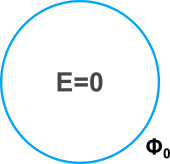
\includegraphics[width=0.3\textwidth]{images/intconduct} % Replace with your image
\end{wrapfigure}
Consideriamo un conduttore chiuso e  cavo (come per esempio un guscio sferico), la sua superficie equipotenziale $\phi_0$ costituisce una condizione al contorno rispetto allo spazio interno in cui si ha l'equazione di Laplace $\nabla^2 \phi =0$. 
La condizione al contorno fa s\`i che la soluzione \`e data da $\phi = k \in \mathbb{R}$, di conseguenza $\bold{E} = - \nabla \phi =0$.
  
\subsection{Metodo delle cariche immagine}

Prendiamo un piano conduttore infinito e poniamo a potenziale nullo $\phi = 0$, e poniamo ad una distanza h una carica puntiforme $q$. Vogliamo descrivere il comportamento del sistema nel suo complesso. 
\begin{figure}[!ht]
\vspace{0.1in}
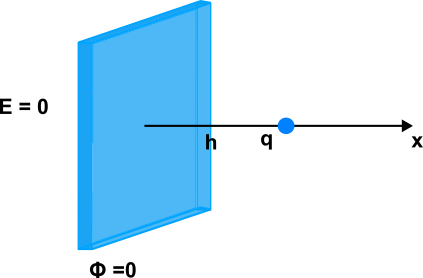
\includegraphics[width = 7cm]{images/chargeplane}	
\centering
\end{figure}

Abbiamo un informazione importante data dal fatto che il piano conduttore \`e messo a terra ovvero ha potenziale nullo. Una configurazione simile in cui si ha un una regione dello spazio in cui il potenziale \`e nullo, la sio ttiene quando si pongono due cariche puntiformi, Q e -Q equidistanziate tra loro, come in figura (1.11)

\begin{figure}[!ht]
\vspace{0.1in}
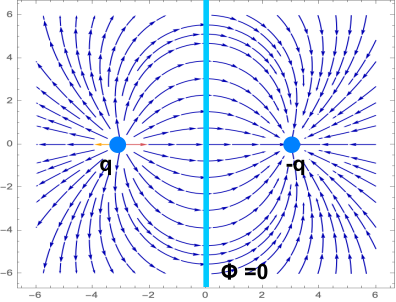
\includegraphics[width = 7cm]{images/imageplane.png}
\centering
\vspace{0.1in}
\caption{}
\end{figure}
Il comportamento del campo magnetico \`e dato dalle linee di campo a sinistra del piano divisore in figura (1.11), ovvero si chiudono sulla superficie, nel caso del problema di partenza, non \`e presente campo $\bold{E} = 0$ in quella parte di spazio divisa dal piano in qui \`e presente la carica $-q$. Vista l'analogia tra i due problemi, poniamo una carica $-q$ in modo simmetricamente opposto ed equidistanziato a q, figura 1.12.
\begin{figure}[!ht]
\vspace{0.1in}
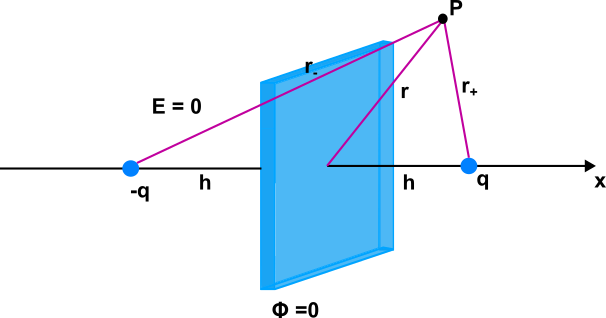
\includegraphics[width = 10cm]{images/mirrormage}
\centering
\vspace{0.1in}
\caption{}
\end{figure}

Il potenziale associato \`e come quello di un dipolo elettrico (nelle prossime sezioni)
\begin{equation}
	\phi(\bold{r})  = \frac{q}{4\pi \varepsilon_0}\left ( \frac{1}{r_+} - \frac{1}{r_-}\right)
\end{equation}
Per tutti i punti in cui $r_+ = r_-$ il potenziale \`e nullo, e coincidono con i punti appartenenti al piano conduttore. Una configurazione di questo tipo ci riconduce al problema di Poisson, dove da una parte \`e presente una distribuzione di carica  e il potenziale sul piano costituisce le condizioni al contorno. Dato che l'equazione ha un unica soluzione, questa coincide con l'equazione (1.40).

Per determinare il valore del campo elettrico sul piano, consideriamo il seguente diagramma delle forze in figura.
\begin{figure}[!ht]
\vspace{0.1in}
\includegraphics[width = 10cm]{images/planechargestudy}
\centering
\vspace{0.1in}
\end{figure}

Le componenti del campo lungo l'asse $\hat{\bold{z}}$ del campo elettrico si annullato. Il campo elettrico lungo $\hat{\bold{x}}$ \`e dato da 
\begin{equation*}
	\bold{E}^{\pm} = -\frac{q}{4\pi \varepsilon_0}\frac{1}{R^2+h^2}\cos \theta \hat{u}_{x} = -\frac{q}{4\pi \varepsilon_0}\frac{h}{(R^2+h^2)^{3/2}} \hat{u}_{x}
\end{equation*}
il campo totale \`e dato da 
\begin{equation*}
	\bold{E} = -\frac{2q}{4 \pi \varepsilon_0} \frac{h}{(h^2 + R^2)^{3/2}} \hat{u}_{z}
\end{equation*}
Dalla legge di Gauss Sappiamo che la distribuzione di carica superficiale $\sigma$ sul piano \`e data da 
\begin{equation*}
	\sigma(R) = - \frac{2q}{4 \pi} \frac{h}{(h^2 + R^2)^{3/2}}
\end{equation*}
Studiando la funzione della distribuzione di carica, si avr\`a una maggiore concentrazione nel centro del piano per R=0.
\begin{figure}[!ht]
\vspace{0.1in}
\includegraphics[width = 8cm]{images/planechagedist}
\centering
\vspace{0.1in}
\end{figure}

\noindent La carica indotta sul piano \`e data da 
\begin{equation*}
	Q_{ind} = \int_{S} \sigma(R) dA
\end{equation*}
dato che la densit\`a di carica dipende dal raggio conviene integrare in coordinate polare sul piano, ovvero $dA = RdRd\theta$, per $\theta \in [0,2\pi]$. L'integrale della carica indotta diventa
\begin{equation*}
	Q_{ind} = -\frac{q}{2 \pi} \int_{0}^{+\infty} \frac{h 2 \pi R}{[R^2+h^2]^{3/2}}dR = -\frac{qh}{2} 
	\Big [-2(R^2+h^2)^{-1/2}\Big ]_{0}^{+\infty} =-q
\end{equation*}
Quindi si ha \textit{induzione totale}, ovvero le linee di campo che escono da $q^+$ si chiudono tutte sul piano.

Abbiamo determinato come si distribuiscono le cariche negative sul piano, ma che cosa succede alle cariche positive?

Mediamente queste non si spostano e sono trascurabili, se consideriamo un disco sul piano, la densit\`a di carica positiva \`e data da 
\begin{equation*}
	\sigma^+ = \frac{q}{2 \pi R^2}
\end{equation*}
se confrontiamo la densit\`a di carica negativa con quella positiva, abbiamo che 
\begin{equation*}
	\frac{\sigma^+}{\sigma^-(0)} = \frac{h^2}{R^2} 
\end{equation*}
se prendiamo $R >> h$, avremo che la carica positiva risulta essere trascurabile. 

Se vogliamo determinare la forza che esercita il piano conduttore sulla carica $q$, questa \`e equivalente alla forza tra due cariche di segno opposto, ovvero
\begin{equation*}
	\bold{F} = q\bold{E} = \frac{q q'}{4\pi \varepsilon_0} \frac{1}{(2h)^2} \hat{u}_{x} = -\frac{q^2}{4 \pi \varepsilon_0} \frac{1}{(2h)^2} \hat{u}_{x}
\end{equation*}
Per determinare l'energia potenziale della configurazione piano-carica, consideriamo l'energia che dovremmo immettere nel sistema per spostare la carica $q$ ad una distanza $h$ dal piano, questa \`e data da 
\begin{equation*}
	U_{piano-q}= W = q\Delta V = -q \int_{h}^{+ \infty} \frac{q}{4\pi \varepsilon_0} \frac{1}{4x^2}dx = \frac{q^2}{4 \pi \varepsilon_0} \frac{1}{4h} = \frac{U_{qq'}}{2}
\end{equation*}
dove l'energia $U_{qq'}$ \`e l'energia d'interazione tra carica immagine $q' = -q$ e $q$. Questa coincide con il lavoro necessario a spostare la carica $q$ ad una distanza $2h$ da $q'$.
\begin{equation*}
	U_{qq'} = -q \int_{2h}^{+\infty} \frac{q'}{4 \pi \varepsilon_0}\frac{1}{x^2}= \frac{qq'}{4 \pi \varepsilon_0}\frac{1}{2h}
\end{equation*}
Il risultato per cui $U_{piano-q} = U_{qq'}/2$ possiamo interpretarlo con il fatto che nella regione di spazio in cui \`e presente la carica immagine il campo elettrostatico \`e nullo, quindi stiamo considerando met\`a del campo dato dall'interazione tra $q$ e $-q$ e quindi anche met\`a dell'energia.

Se allontaniamo la carica sonda $q$ dal piano, la distribuzione di carica negativa formatasi dall'interazione si sparpaglia nel conduttore per mantenere una configurazione in cui il potenziale sul piano \`e nullo. Il lavoro sulle cariche che si spostano all'interno di un conduttore \`e nullo , perch\`e dato $\phi = k \in \mathbb{R}$, allora $W_{cond} = 0$. Possiamo pensare che le cariche si muovano in direzione ortogonale rispetto al campo elettrostatico.

\section{Energia del campo elettrostatico}

Nelle sezioni precedenti abbiamo calcolato l'energia potenziale associata ad una configurazione di cariche. Possiamo vedere una distribuzione di carica continua come un aggregato di tante cariche, che interagiscono tra di loro esercitando una forza di natura Coulombiana e una di coesione, che permette di mantenere la configurazione. Dato che le cariche sono statiche, avremo che 
\begin{equation*}
	\bold{F} = 0 \quad \Rightarrow  \quad q\bold{E} + \bold{F}_{altro} = 0 \quad  \Rightarrow  \quad \bold{F}_{altro} =-q \bold{E}
\end{equation*} 
di conseguenze le forze di coesione avranno pari intensit\`a e direzione, ma verso opposto; inoltre la loro origine \`e di natura elettrica e legata alle cariche atomiche.

Vogliamo dare una definizione alternativa all'energia potenziale elettrostatica calcolando l'energia necessaria ad assemblare la configurazione di carica. 
\newline

\noindent In un certo qual modo pensare di portare delle cariche da infinito tutte insieme e di darle una forma sferica, \`e equivalente ad esercitare contemporaneamente una pressione su tutta una superficie  sferica riducendone uniformemente il raggio. Quindi consideriamo di avere una sfera cava di raggio R e densit\`a di carica superficiale $\sigma $, il campo generale coincide con quello di una carica puntiforme
\begin{equation*}
\bold{E}(r) = \left \{ \begin{array}{l}
	 \frac{1}{4 \pi \varepsilon_0} \frac{\sigma 4 \pi R^2}{r} \hat{u}_{r} \quad r \geq R\\[0.3cm]
	0 \quad r < R
\end{array}\right.
\end{equation*}
e quindi sulla superficie esterna si ha 
\begin{equation*}
	\bold{E} =  \frac{\sigma}{\varepsilon_0} \hat{u}_{r}
\end{equation*}
Le cariche per un area infinitesima $da$ sulla superficie della sfera, esercitano tra di loro una forza di Coulomb 
\begin{equation*}
	d\bold{F} = dq \bold{E}
\end{equation*}
\begin{wrapfigure}{r}{0.4\textwidth} % 'r' for right, 'l' for left
    \centering
    \includegraphics[width=0.4\textwidth]{images/pressure} % Replace with your image
\end{wrapfigure}
Per comprimere la sfera di un tratto $d\bold{r}$, modificandone il raggio bisogna compiere un lavoro sul sistema 
\begin{equation*}
	dU = -dW = -\bold{F} \cdot d\bold{r}
\end{equation*}  
 Le cariche presenti sulla superficie per la sfera con raggio R, si ritroveranno dopo la compressione ad una distanza mediamente inferiore, generando un campo elettrico l\`a dove prima non era presente. Per esprimere dU in funzione del campo elettrico dovuto alla distribuzione delle cariche, abbiamo bisogna di determinare l'espressione della forza $\bold{F}$ d'interazione delle cariche sulla superficie di raggio ridotto.
 
\begin{wrapfigure}{l}{0.4\textwidth} % 'r' for right, 'l' for left
    \centering
    \includegraphics[width=0.4\textwidth]{images/superficie} % Replace with your image
\end{wrapfigure}
Per calcolarla consideriamo uno strato di spesso molto piccolo $d\bold{r}$, equivalente alla quanti\`a di quanto si \`e ridotto il raggio della sfera. Al suo interno \`e presente una densit\`a di carica volumica $\rho$ uniforme e sufficiente affinch\`e si abbia che $ \sigma = \rho dr $ per qualsiasi dr scelto. Si dimostra facilmente usando la legge di Gauss che l'intensit\`a del campo elettrico \`e zero sulla superficie interna dello strato e cresce linearmente fino a raggiungere il valore $4 \pi \sigma $ sulla superficie esterna. 
Il valore medio del campo elettrico nello strato, e di conseguenza la forza media agente su una carica unitaria interna allo strato, \`e 
\begin{equation*}
	\langle E \rangle = \frac{1}{2}(E_{itn} + E_{ext}) = \frac{\sigma}{2\varepsilon_0} 
\end{equation*}
dato che $E_{int} = 0$. La forza agente complessivamente per ogni porzione di superficie $dA$ e larghezza $dr$, sar\`a data dalla relazione 
\begin{equation*}
	F = \int_{o}^{r}dF = \int_{0}^{r}dq \; E = \int_0^r dr\; \rho E da
\end{equation*}
 dove $dq = \rho \cdot da \cdot dr$. Sappiamo che $d\sigma = \rho dr$ utilizzando la legge di Gauss abbiamo deduciamo che $d \sigma = \varepsilon_0 \;dE$, di conseguenza possiamo riscrivere l'integrale precedente rispetto al campo elettrico
 \begin{equation*}
 	P = \frac{F}{da} = \varepsilon_0 \int_{E_{int}}^{E_{ext}} dE \; E = \frac{1}{2} \varepsilon_0 (E_{ext}^2-E_{int}^2) = \frac{1}{2} \varepsilon_0(E_{ext} + E_{int})\Delta E
 \end{equation*}
 dove $\Delta E = \sigma / \varepsilon_0$ e quindi possiamo concludere che la \textit{pressione elettrostatica} \`e data da 
 \begin{equation*}
 	P = \frac{\sigma^2}{2 \varepsilon_0}
 \end{equation*}
 La direzione della forza \`e verso l'esterno della superficie, indipendentemente dal segno della carica dato che \`e quadratica nell'espressione.
 
 Dalla pressione possiamo determinare la densit\`a di energia elettrostatica immagazzinata all'interno del volume $dV = 4\pi R^2 dr$, dato che 
 \begin{equation*}
 	dU = - \bold{F} \cdot d \bold{r} = \frac{\sigma^2}{\varepsilon_0} 4 \pi R^2dr
 \end{equation*}
 che possiamo riscrivere come 
 \begin{equation*}
	dU = \frac{1}{2} \varepsilon_0 E^2 (4\pi R^2dr) \quad \Rightarrow  	u_e = \frac{dU}{dV} = \frac{1}{2}\varepsilon_0 E^2
 \end{equation*}
Ora che abbiamo determinare la quantit\`a di energia presente per unit\`a di volume nello spazio, possiamo calcolare l'energia, integrando sul volume, e quindi definiamo
\begin{equation}
	U = \frac{1}{2} \varepsilon_0 \int_{V} d\nu \; E^2
\end{equation}

\section{Dipolo elettrico}

Un \textit{dipolo} consiste in un sistema di due cariche Q e -Q poste a una distanza $d$. La prima carica \`e posizionata in $d/2$ e la seconda in $-d/2$. Il potenziale non \`e altro che la somma dei potenziali di ciascuna carica
\begin{equation*}
	\phi(r) = \frac{Q}{4 \pi \varepsilon_0} \left( \frac{1}{r_1} - \frac{1}{r_2}\right)
\end{equation*}
Prendiamo un punto P nello spazio  affinch\`e la sua distanza radiale $r$ sia molto pi\`u grande della distanza tra le due cariche. Riscriviamo le congiungenti tra le cariche e P rispetto ad $r$ nel seguente modo
\begin{equation*}
	r_1 = r + \frac{d}{2}\cos\theta \quad \text{e} \quad
	r_2 = r - \frac{d}{2}\cos \theta 
\end{equation*} 
l'espressione del potenziale diventa 
\begin{equation*}
	\phi(r) = \frac{Q}{4 \pi \varepsilon_0} \left(\frac{1}{r + d/2 \cos\theta } - \frac{1}{r - d/2 \cos\theta} \right) = \frac{Q}{4 \pi \varepsilon_0} \frac{d \cos \theta }{r^2 - d^2/4\cos \theta}\simeq \frac{Qd}{4 \pi \varepsilon_0} \frac{ \cos \theta }{r^2}
\end{equation*}
dato che siamo sotto l'ipotesi in cui $r >> d$ si \`e sviluppato in potenziale con Taylor arrestandosi al primo ordine .
Alcune osservazioni:
\begin{enumerate}

\item Nel potenziale compare il termine $ p=Qd$ che prende il nome di \textit{momento di dipolo}.

\item Un dipolo ideale \`e dato da $d \to 0$ e $q \to \infty $ con il momento di dipolo che assume un particolare valore finito. A differenza del potenziale di una carica puntiforme quello del dipolo \`e proporzionale a $1/r^2$ decrescendo molto pi\`u velocemente; questo \`e dovuto al fatto che il potenziale delle due cariche opposte tende a cancellarsi quando $r >> d$. L'unico contributo restante \`e quello dovuto alla distanza tra due cariche leggermente differenti.
\item Il potenziale \`e proporzionale al $\cos \theta $, questo ci dice che in direzione $\perp$ al dipolo il potenziale \`e $\phi(r,\pm \pi/2) = 0$, mentre per una direzione parallela il potenziale \`e massimo.

\end{enumerate}

Utilizzando le coordinate sferiche per l'operatore gradiente determininato il campo elettrostatico generato dalla configurazione di carica
\begin{equation*}
	\bold{E} = -\nabla \phi = - \left [ \frac{\partial \phi }{\partial r}\hat{u}_r + \frac{1}{r} \frac{\partial \phi}{\partial \theta}\hat{u}_{\theta} \right ] = \frac{Qd}{4 \pi \varepsilon_0}\frac{1}{r^3} [2 \cos \theta \hat{u}_{r} + \sin\theta \hat{u}_{\theta}]
\end{equation*}

 
\begin{figure}[!ht]
\vspace{0.1in}
\includegraphics[width = 8cm]{images/dipol1}	
\centering
\caption{Campo elettrico generato da un dipolo}
\end{figure}

\newpage

\section{Esempi ed esercizi}

\subsection{Carica puntiforme in prossimit\`a di una sfera conduttrice (Esame 23/06/2020)}

\begin{wrapfigure}{r}{0.4\textwidth} % 'r' for right, 'l' for left
    \centering
    \includegraphics[width=0.4\textwidth]{images/spherecharge} % Replace with your image
\end{wrapfigure}
Si consideri un sistema dove si ha una carica puntiforme $q$ ad una distanza $a$ da un conduttore sferico con massa a terra di raggio $r$. Vogliamo calcolare il lavoro necessario ad allontanare la carica da $a$, verso infinito.

\begin{proof}
	Per risolvere il problema possiamo usare il metodo della carica immagine, ovvero andiamo a collocare una carica immaginaria $Q$ all'interno del conduttore, affinch\`e il potenziale $\phi$ sulla superficie della sfera sia nullo. Di conseguenza abbiamo bisogno di determinare per quali valori $Q$ e in quale posizione $x$ tale condizione \`e verificata.
\newline

Ipotizziamo si posizionare le due cariche $Q$ e $q$ in due generici punti $(b,0,0)$ dove $b < r$ e $(a,0,0)$ per $a >r$. Il potenziale complessivo del sistema a due cariche \`e dato da 
\begin{equation*}
	V(x,y,z) = \frac{1}{4 \pi \varepsilon_0} \left [ \frac{q}{\sqrt{(x-a)^2 + y^2 + z^2}} + \frac{Q}{\sqrt{(x-b)^2+y^2+z^2}} \right]
\end{equation*}
Imponendo la condizione $\phi = 0$, abbiamo che 
\begin{align*}
	& \frac{q}{\sqrt{(x-a)^2 + y^2 + z^2}} =- \frac{Q}{\sqrt{(x-b)^2+y^2+z^2}} \iff \frac{Q^2}{q^2} = \frac{(x-b)^2 + y^2 + z^2}{(x-a)^2 + y^2 + z^2} \\[0.5cm]
	& \Rightarrow \frac{Q^2}{q^2} = \frac{x^2 + y^2 +z^2 +2bx + b^2}{x^2 + y^2 +z^2 + 2ax + a^2} = \frac{r^2 - 2bx +b^2}{r^2 - 2ax +a^2} 
	\Rightarrow \\[0.5cm]
	& \Rightarrow \frac{Q^2}{q^2}r^2 + \frac{Q^2}{q^2}a^2 - 2\frac{Q^2}{q^2}ax =  r^2 - 2bx +b^2 \Rightarrow 
\end{align*}
\begin{align}
	& \Rightarrow r^2 \left( \frac{Q^2}{q^2}-1 \right) = -\frac{Q^2}{q^2}a^2 +b^2 + 2x \left(\frac{Q^2}{q^2}a - b\right)
\end{align}
l'equazione (1.42) assume un espressione semplifica se poniamo l'ultimo addendo nullo, ovvero $b = (Q^2/q^2)a$, e quindi possiamo riscrivere l'equazione nel seguente modo:
\begin{equation*}
	r^2 \left( \frac{b}{a} -1\right) = -ab + b^2  = ab\left (\frac{b}{a}-1 \right) \Rightarrow r^2 = ab
\end{equation*}
troviamo dunque che la posizione della carica Q affinch\`e $\phi(x,y,z) = 0$ \`e data  da 
\begin{equation*}
\boxed{
	b = \frac{r^2}{a}
	}
\end{equation*}
ci manca ora da determinare la carica immagine $Q$  all'interno del conduttore sferico affinch\`e $\phi(R) = 0$. Per farlo riscriviamo l'espressione del potenziale complessivo con il risultato trovato,
\begin{equation*}
	\phi(x,y,z) = \frac{1}{4 \pi \varepsilon_0} \left [ \frac{q}{\sqrt{(x-a)^2+y^2+z^2}} + \frac{Q}{\sqrt{(x-r^2/a)^2 +y^2+z^2}}\right]
\end{equation*}
e imponiamo che per $\phi(r,0,0) = 0$  e quindi abbiamo l'equazione 
\begin{equation*}
	\phi(r) = \frac{1}{4 \pi \varepsilon_0} \left [ \frac{q}{|r-a|} + \frac{Q}{|r - \frac{r^2}{a}|}\right] = 0
\end{equation*}
dato che $a >R$ si ha che $|r-a| = -(r-a)$.L'equazione diventa
\begin{align*}
	& Q = \frac{q}{r-a}\left ( r-\frac{r^2}{a}\right)\\[0.5cm] 
	& \Rightarrow \boxed{Q = -\frac{r}{a}q}
\end{align*}
dunque per un potenziale del seguente tipo 
\begin{equation*}
	V(x,y,z) = \frac{q}{4 \pi \varepsilon_0} \left [ \frac{1}{\sqrt{(x-a)^2 +y^2 + z^2}} - \frac{r}{a}\frac{1}{\sqrt{(x- r^2/a)^2+y^2 +z^2}}\right]
\end{equation*}
abbiamo che \`e soddisfatta la condizione che $\phi(r) = 0$.

Infine possiamo rispondere alla domanda dell'esercizio dove il lavoro per muovere una carica puntiforme da $a$ ad $\infty$ \`e dato da
\begin{equation*}
	W = q \phi(a) = \frac{q^2}{4 \pi \varepsilon_0} \frac{r}{a^2-r^2} 
\end{equation*}
siccome all'interno della sfera conduttrice non c'\`e campo, per il sistema originale dobbiamo considerare met\`a dell'energia trovata e quindi
\begin{equation*}
	W' = \frac{1}{2}W = \frac{q^2}{4 \pi \varepsilon_0} \frac{r}{a^2-r^2}
\end{equation*}

\end{proof}

Che cosa succede se consideriamo la sfera conduttrice scarica e la rimuoviamo dalla messa a terra ?

 \begin{wrapfigure}{l}{0.4\textwidth} % 'r' for right, 'l' for left
    \centering
    \includegraphics[width=0.3\textwidth]{images/spherecharge1} % Replace with your image
\end{wrapfigure}

Avremo che sulla superficie della sfera si crea una distribuzione uniforme di carica $Q'' = -Q$ tale per cui la carica netta su di essa \`e $Q' = Q + Q'' = 0 $ e quindi il conduttore sferico \`e neutro. Questo equivale a porre una seconda carica immagine $Q''$ al centro della sfera. 

Applicando il principio di sovrapposizione per il potenziale di ciascuna carica e considerando l'orgine del sistema di riferimento con il centro della sfera, avremo che 
\begin{equation*}
	\phi(x,y,z) = \frac{q}{4 \pi \varepsilon_0} \left [ \frac{1}{\sqrt{(x-r)^2 + y^2 +z^2}} - \frac{R}{r}\frac{1}{\sqrt{(x-R^2/r)^2 + y^2 + z^2}} + \frac{R}{r} \frac{1}{\sqrt{x^2+y^2+z^2}}\right]
\end{equation*}
Per determinare il lavoro necessario a spostare la carica da $r$ a $+ \infty$ calcoliamo
\begin{equation*}
	W = q\phi(r,0,0) = \frac{q^2R}{4 \pi \varepsilon_0} \left(\frac{1}{r^2-R^2} - \frac{1}{r^2} \right)
\end{equation*}
l'energia trovata \`e quella della configurazione delle cariche, per determinare quella associata alla sfera conduttrice neutra, dobbiamo ricordare che internamente il campo \`e nullo e dunque il lavoro necessario \`e la met\`a di W.
\begin{equation*}
	W' = W/2 = \frac{q^2R}{8 \pi \varepsilon_0} \left(\frac{1}{r^2-R^2} - \frac{1}{r^2} \right)
\end{equation*}

\subsection{Esercizio 2}











